\documentclass[aspectratio=169]{beamer}
\usepackage{graphicx} % Required for inserting images
\usepackage{outlines}
\usepackage{svg}
\usepackage{tikz}
 \usetikzlibrary{calc} 
\usepackage{qrcode}
\usepackage{xcolor}

% ---- Chinese characters --------------------------------------------------------
\usepackage{xeCJK} % for Chinese, compiling by XeLaTex
\usepackage{fontspec} %設定字體
% Fandol font (the default)  not shown "內"
\setCJKmainfont{AR PL UMing TW MBE} % AR PL UMing TW MBE or "UKai" https://www.overleaf.com/learn/latex/Questions/Which_OTF_or_TTF_fonts_are_supported_via_fontspec%3F#Chinese
%BiauKai} %標楷體 from macOS %設定中文為系統上的字型,而英文不去更動,使用原TeX字型

\XeTeXlinebreaklocale "zh"
\XeTeXlinebreakskip = 0pt plus 1pt %這兩行一定要加,中文才能自動換行

%\usepackage{CJKutf8}
%\newcommand{\cntext}[1]{\begin{CJK*}{UTF8}{bkai}#1\end{CJK*}}
%----------------------------------------------------------------------------------------

\usetheme{Warsaw}

\title{Holistic Healthcare from Taiwan Medical Mission \\ in the Republic of Somaliland}

%\title{KOMA_TMM_chief_keynote_20230713_forTMWH}
\author{Dr. Tex Li-Hsing Chi, D.D.S., Ph.D. \\
        Oral and Maxillofacial surgeon \\
        Translational Medicine}
\institute{Wanfang Hospital, managed by Taipei Medical University}
\date{13 July 2023}

%%%
\makeatletter
\setbeamertemplate{headline}
{
  \leavevmode%
  \hbox{%
  \begin{beamercolorbox}[wd=.5\paperwidth,ht=2.5ex,dp=1.125ex]{section in head/foot}%
    \insertsectionnavigationhorizontal{.5\paperwidth}{\hskip0pt plus1filll}{}%
  \end{beamercolorbox}%
  \begin{beamercolorbox}[wd=.4\paperwidth,ht=2.5ex,dp=1.125ex,right]{subsection in head/foot}%
    \usebeamerfont{subsection in head/foot}\insertsubsectionhead\hspace*{2ex}
  \end{beamercolorbox}%
  \begin{beamercolorbox}[wd=.1\paperwidth,ht=2.5ex,dp=1.125ex,left]{subsection in head/foot}%
    %\includesvg[height=2.5ex]{TMM_logo.svg}
  \end{beamercolorbox}}%
  \vskip0pt%
}
\makeatother
%%%


%%%
\makeatletter
\setbeamertemplate{footline}
{
  \leavevmode%
  \hbox{%
  \begin{beamercolorbox}[wd=.333333\paperwidth,ht=2.25ex,dp=1ex,center]{author in head/foot}%
    %\usebeamerfont{author in head/foot}\insertshortauthor
    Chief Tex of TMM
  \end{beamercolorbox}%
  \begin{beamercolorbox}[wd=.333333\paperwidth,ht=2.25ex,dp=1ex,center]{title in head/foot}%
    Holistic Healthcare from TMM
  \end{beamercolorbox}%
  \begin{beamercolorbox}[wd=.333333\paperwidth,ht=2.25ex,dp=1ex,right]{date in head/foot}%
    \usebeamerfont{date in head/foot}\insertshortdate{}\hspace*{2em}
    \insertframenumber{} / \inserttotalframenumber\hspace*{2ex} 
  \end{beamercolorbox}}%
  \vskip0pt%
}
\makeatother
%%%


%%%
\setbeamertemplate{frametitle}
{
    \nointerlineskip
    \begin{beamercolorbox}[sep=0.3cm,ht=1.8em,wd=\paperwidth]{frametitle}
        \vbox{}\vskip-2ex%
        \strut\insertframetitle\strut
        \hfill
        \includesvg[height=1.7em]{TMM_logo.svg}
        \vskip-0.8ex%
    \end{beamercolorbox}
}
%%%

\begin{document}
%\begin{abstract}
%The Taiwan Medical Mission (TMM) is an overseas project that helps the people of Somaliland get health care since 2022/07/28. The TMM is a medical mission that helps people of the people in the Somalia region get medical care. It is also a telepathology project with a pathologist through digital whole-slide images (WSIs). This project supports medical staffs who work at the Hargeisa Group Hospital (HGH) and a hospital in Somalia. This project aims to support medical staff members who work in the HGH. In addition, the TMM supports the health care system in the Taiwan medical mission.
%\end{abstract}

%\begin{CJK*}{UTF8}{gbsn}

\begin{frame}
\titlepage
\end{frame}

\begin{frame}
\frametitle{Outline}

\begin{columns}
\column{0.4\textwidth}
\tableofcontents

\column{0.6\textwidth}
\includesvg[width=0.7\textwidth]{TMM_logo.svg}

\end{columns}


\end{frame}


%%%%%
\section{Overture}

\begin{frame}{序曲}
    \begin{center}
        \includesvg[width=0.8\textwidth]{TRO_Somaliland_font_ZongKai.svg}
    \end{center}
\end{frame}

\begin{frame}{序曲}

\begin{columns}
\column{0.4\textwidth}
    \begin{outline}
        這裡是外交先鋒,\\
        這裡是戰地後盾,\\
        這裡是,1973年代的臺灣,\\
        我們沒有參與過去的臺灣,\\
        但我們正在撰寫索蘭的醫療史,\\
        Taiwan Mission 是,\\
        不拿槍的幕後英雄。\\
    \end{outline}

\column{0.6\textwidth}
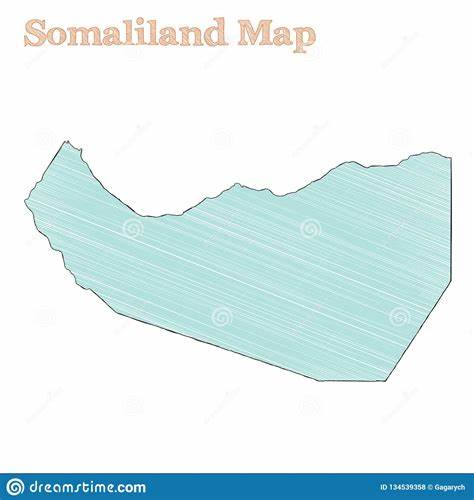
\includegraphics[width=0.7\textwidth]{Somaliland.jpeg}
\end{columns}

\end{frame}


%%
\section{Introduction}
\begin{frame}
\frametitle{Introduction}
% Add content here
\begin{outline}
    

\1 The Taiwan Medical Mission (TMM) is an overseas project that helps the people of Somaliland get health care since 2022/07/28.
    \2 our brother mission: TMM in the Kingdom of Eswatini since 2008 leaded by Dr. Tu Chi-cheng (杜繼誠團長)
\1 The team consists of 
    \2 an obstetrician (林威霖), a registered nurse (黃全賢), a emergency doctor (巫昀祐), and an oral and maxillofacial surgeon (祁力行團長); a administrator (程書螢). 
    \2 to support medical staffs who work at the Hargeisa Group Hospital (HGH), Hargeisa, Somaliland
%\1 TMM members are willing to adapt to different cultures and settings and work with limited resources and facilities.



\end{outline}

\qrcode[height=0.7in]{https://youtu.be/uOwzikPw-0U}
2023/05 消失的國界(三立電視 東非現場)

\end{frame}


\begin{frame}{Medical affairs - 消失的國界}
    \begin{center}
        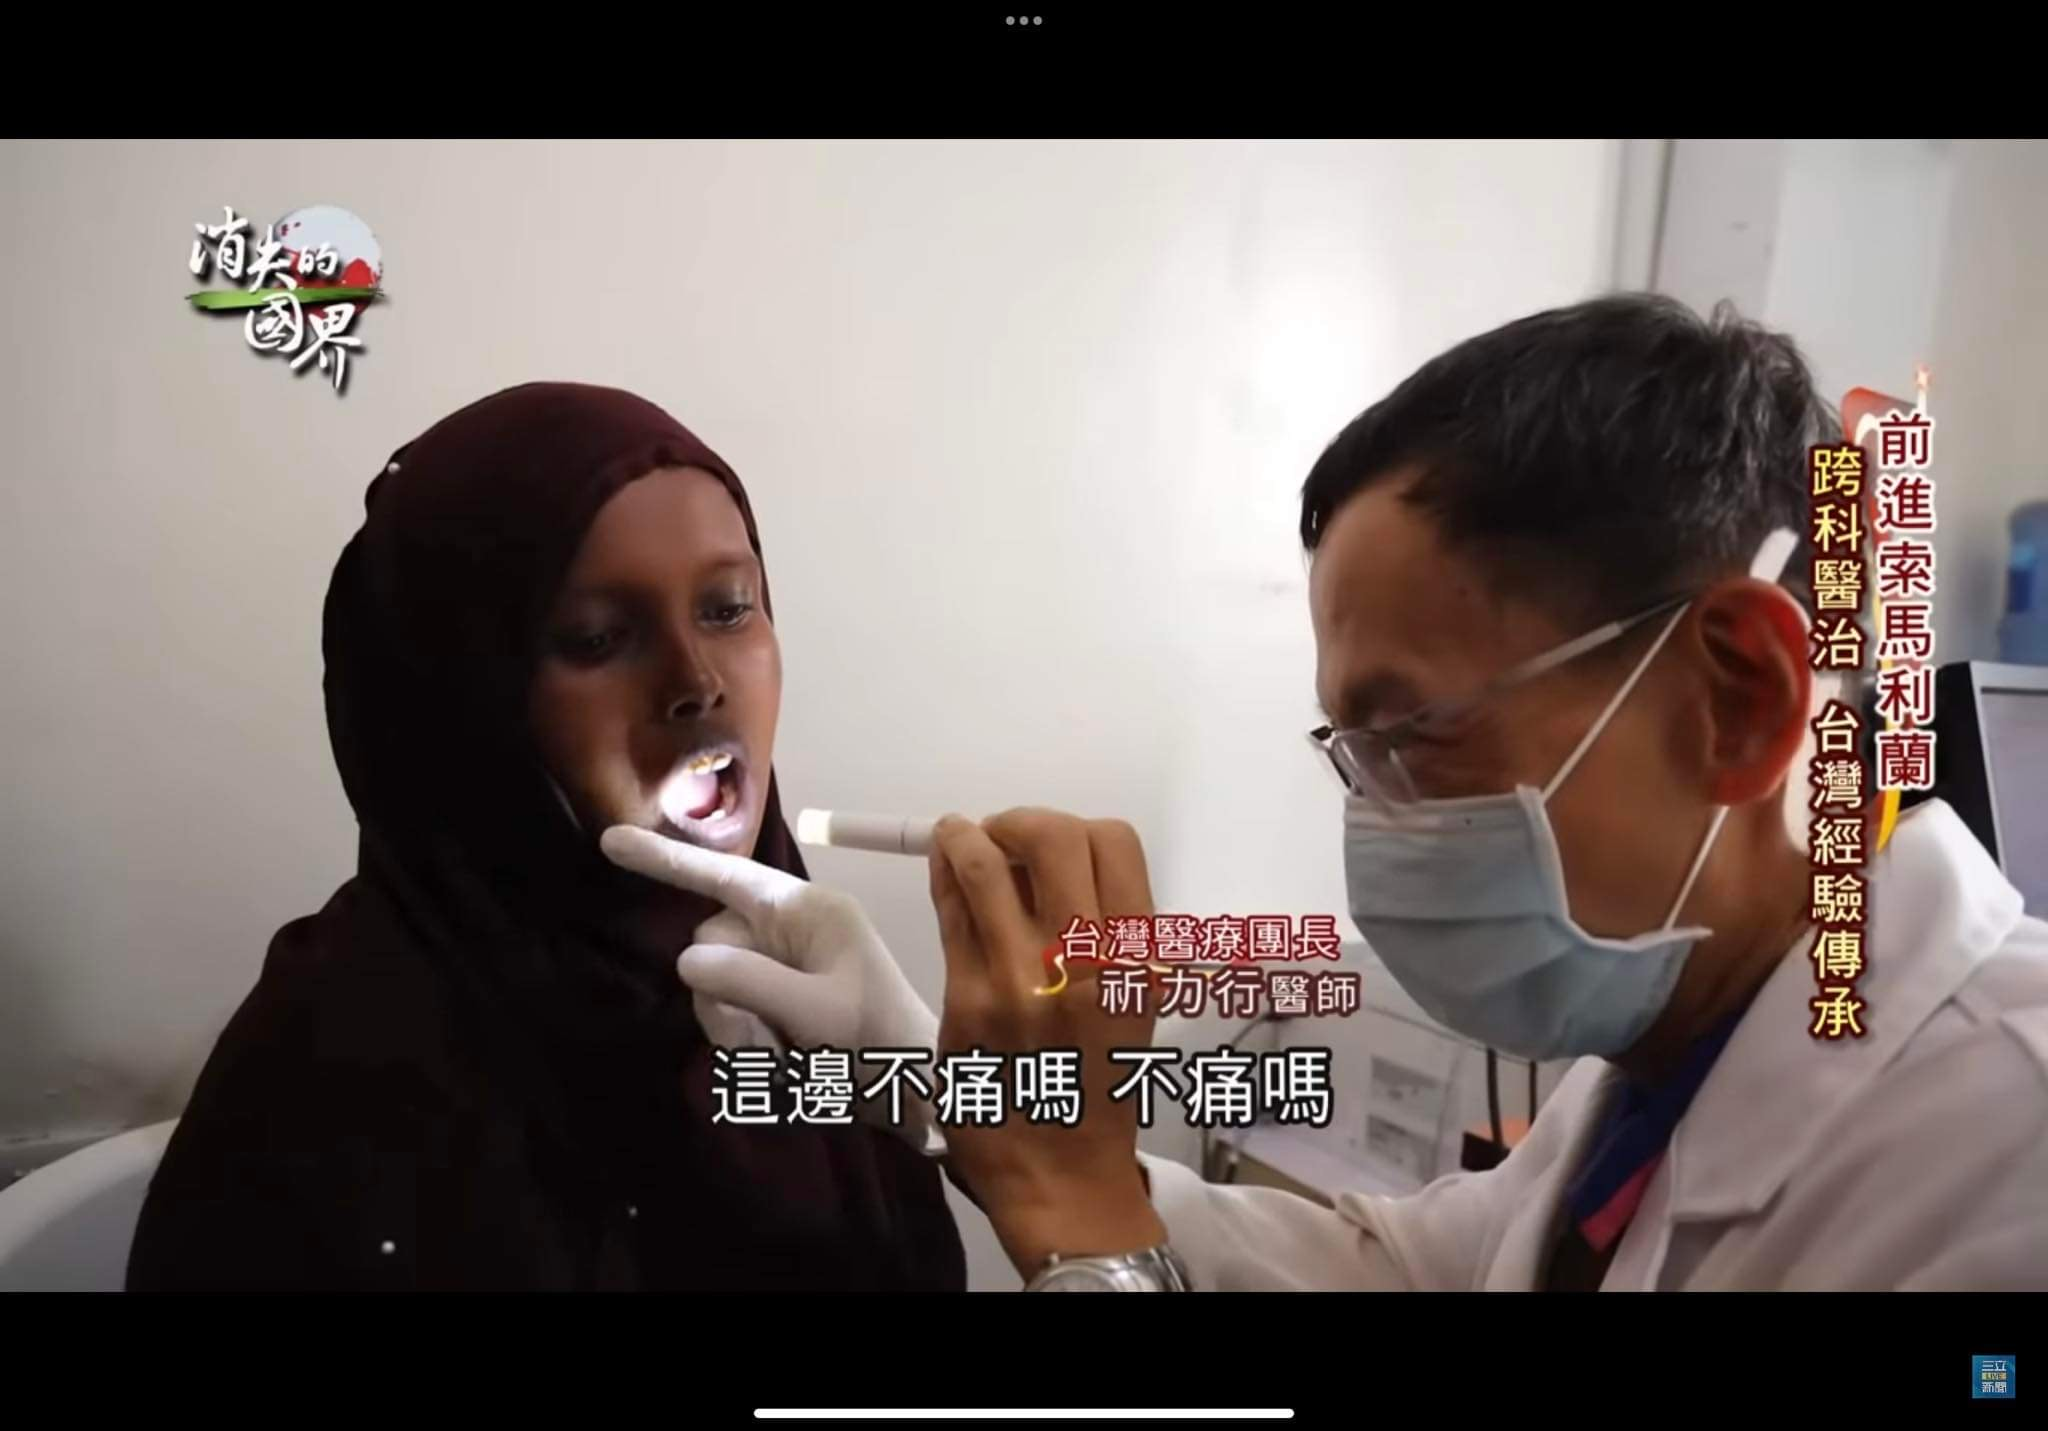
\includegraphics[width=0.8\textwidth]{IMG_4940(1).jpeg}

    \end{center}
\end{frame}

\begin{frame}{Medical affairs - 消失的國界}
\begin{center}
    
\begin{tikzpicture}
    \node[anchor=south west,inner sep=0] (image) at ($(current page.center)+(-2cm,0)$) {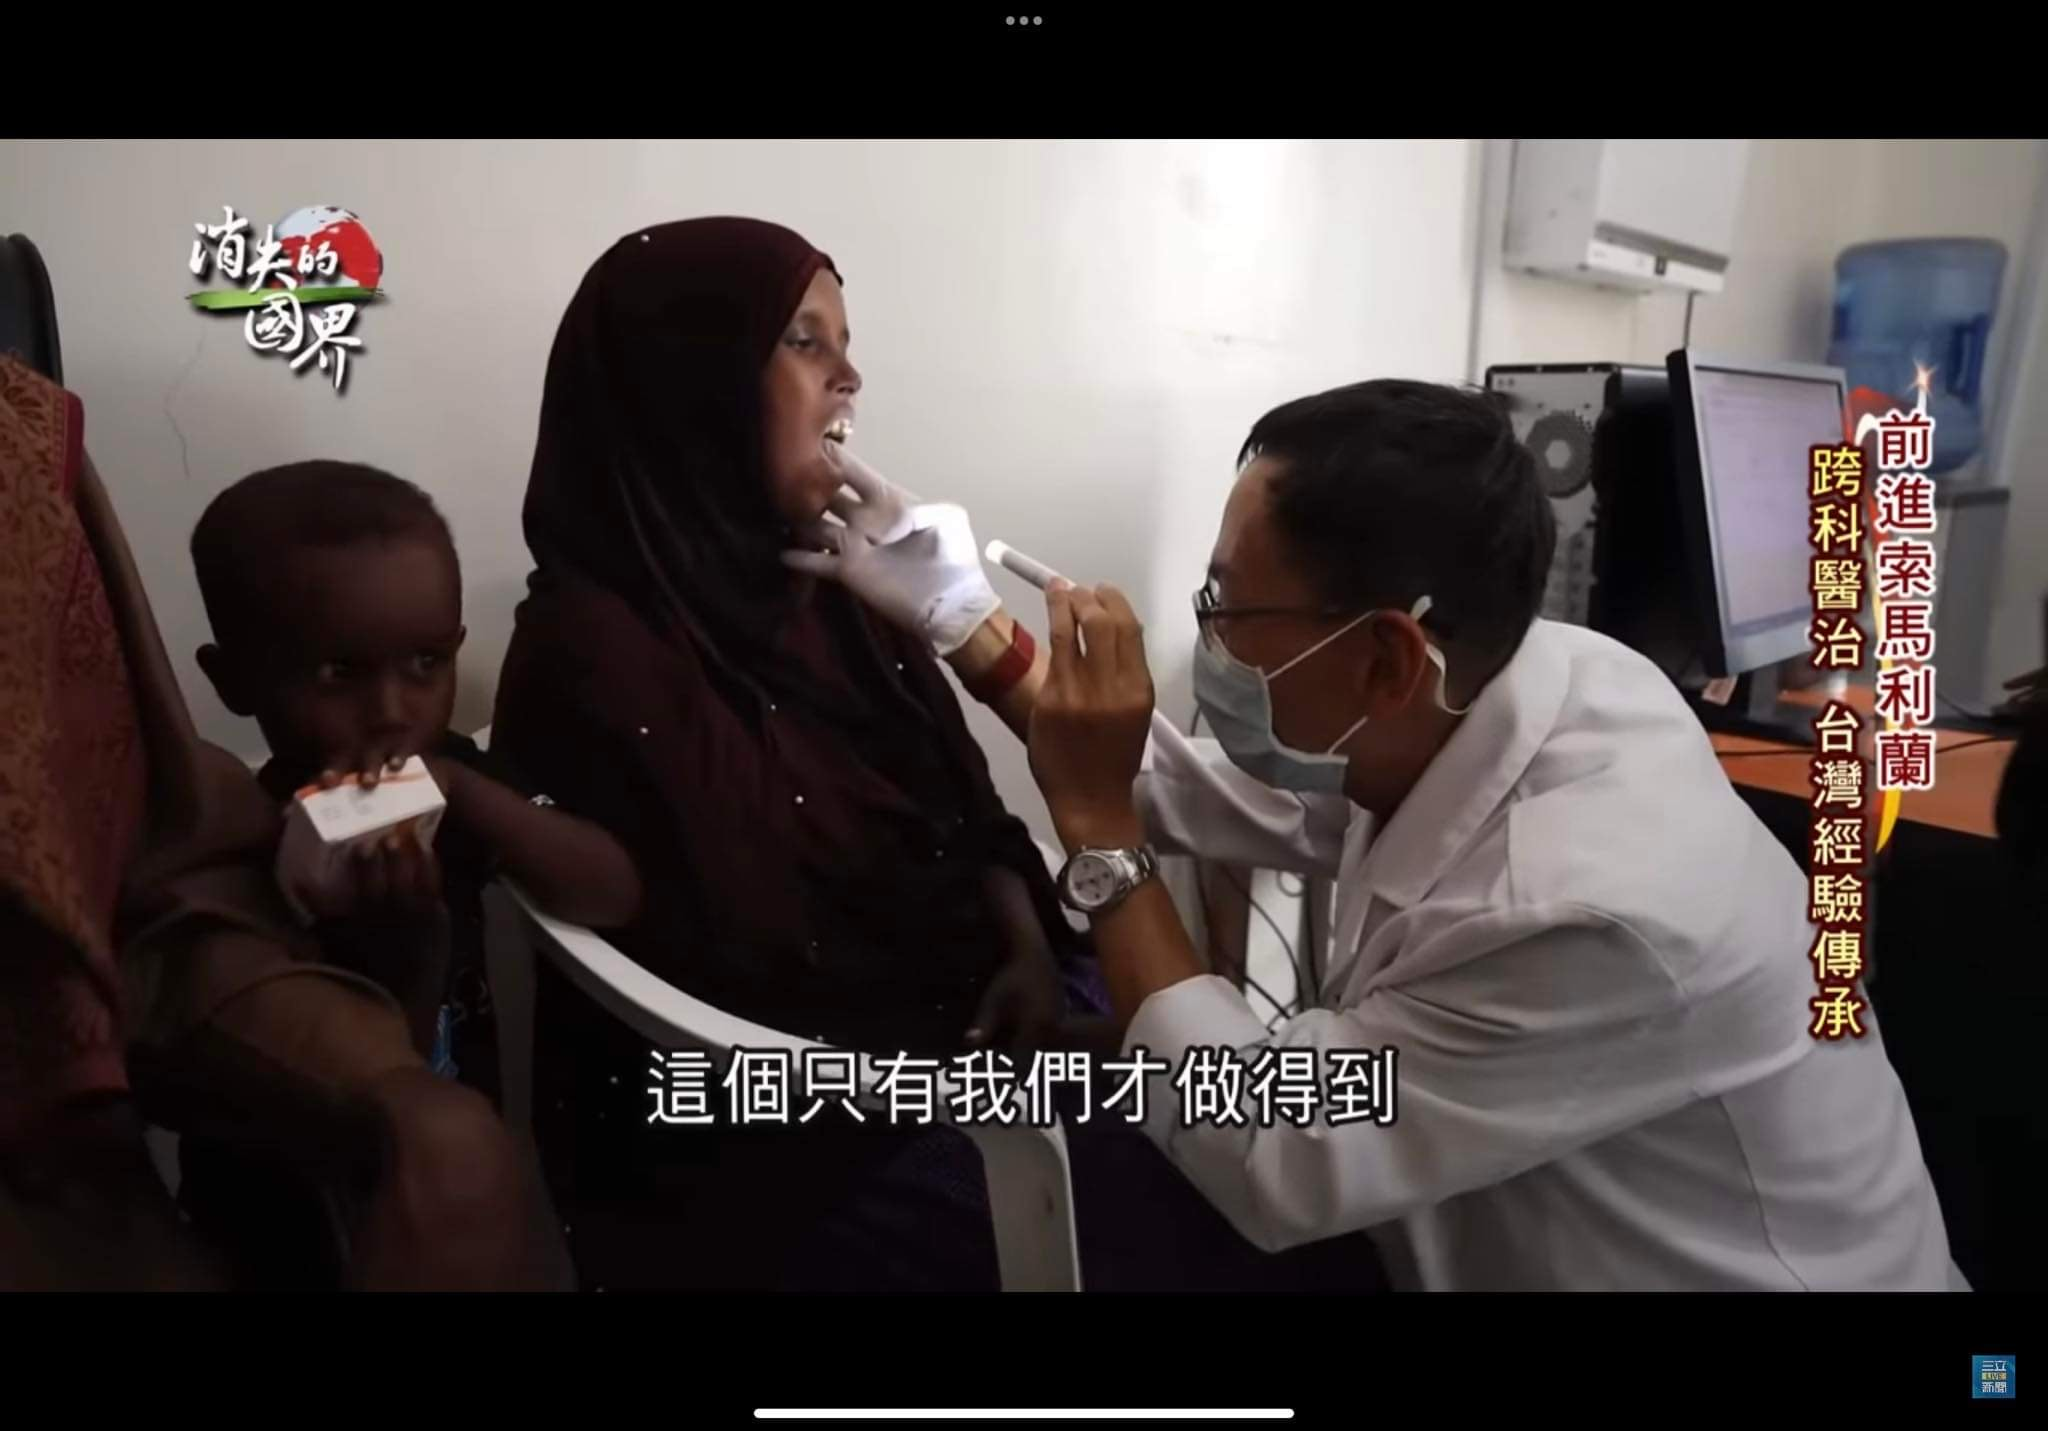
\includegraphics[width=0.8\textwidth]{IMG_4949(1).jpeg}};
    \begin{scope}[x={(image.south east)},y={(image.north west)}]
        \fill[white] (0.25,0.60) circle (0.04);
    \end{scope}
\end{tikzpicture}

\end{center}

\end{frame}


\begin{frame}{Two TMMs in the World}
\begin{tikzpicture}
\node[anchor=west] (africa) at (0,0) {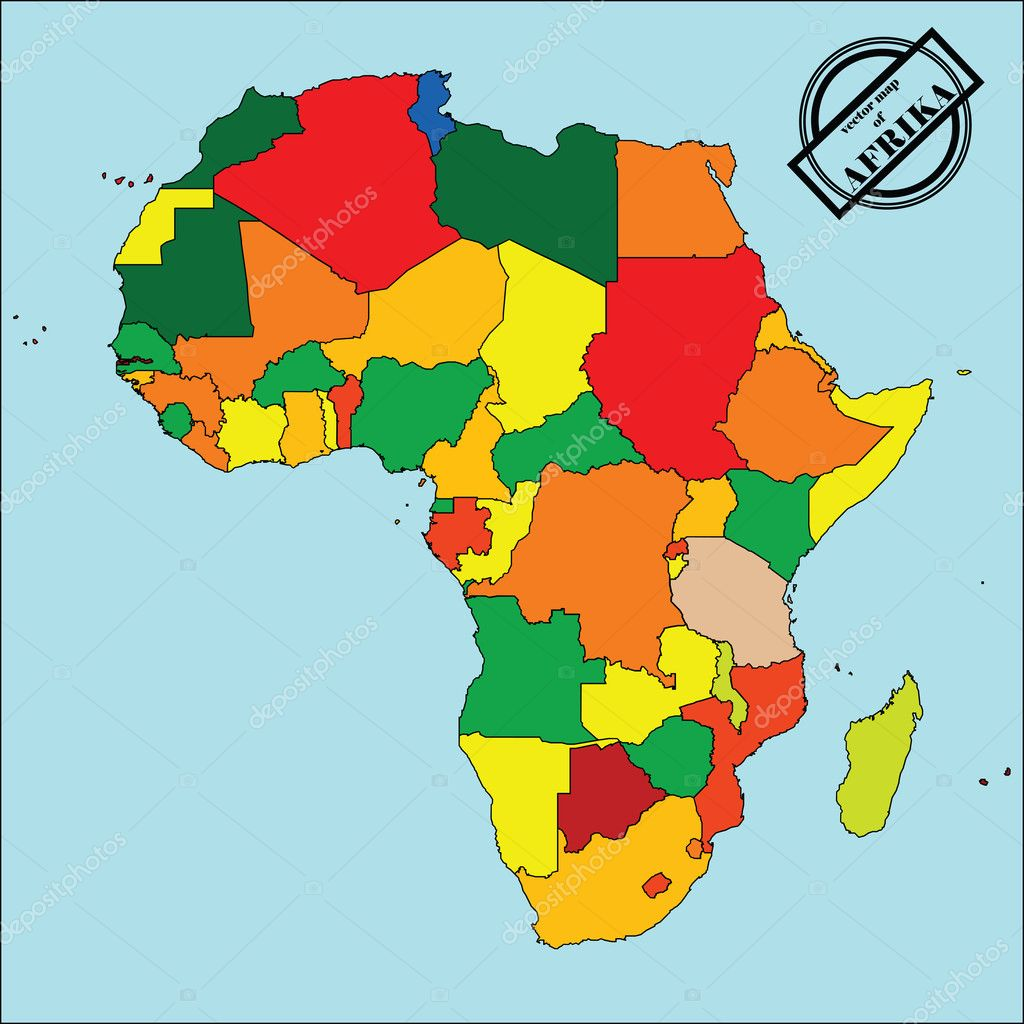
\includegraphics[width=0.4\textwidth]{worldMap_Africa.jpeg}};

\node[anchor=south west] (TMM_2022) at ([yshift=+2.0cm]africa.east) {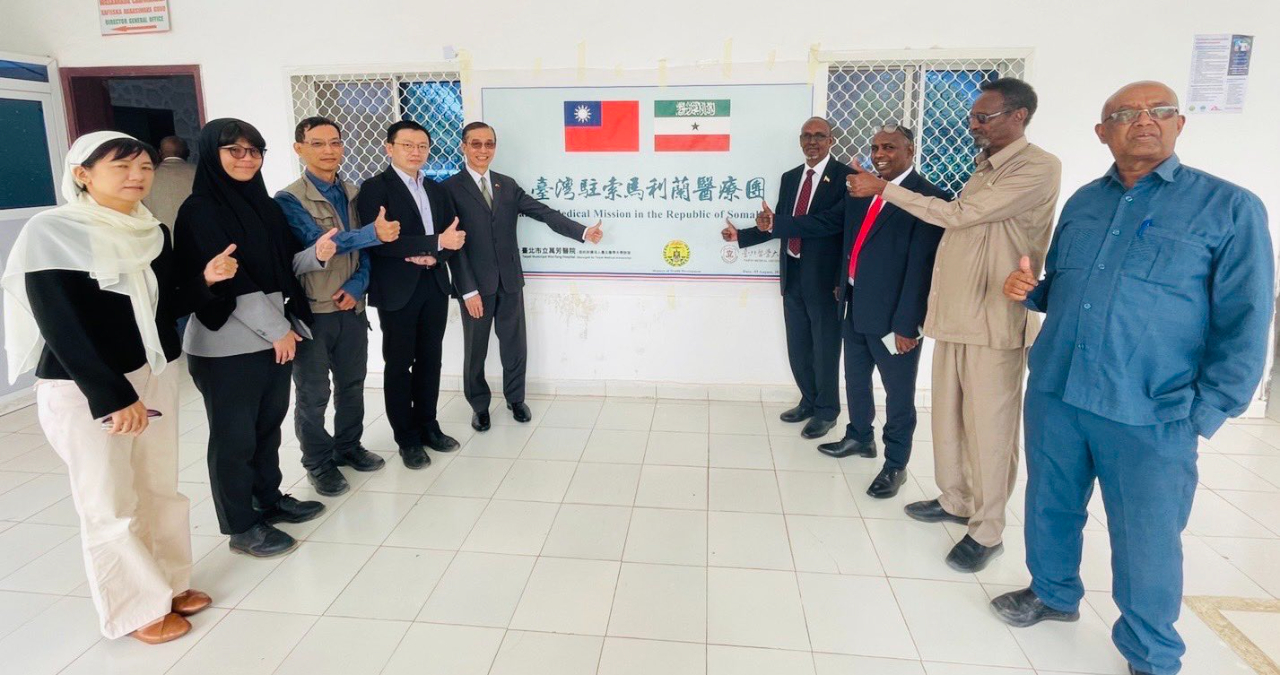
\includegraphics[width=0.30\textwidth]{TMM2022July.jpeg}};

\node[anchor=south west] (TMM_sln) at ([xshift=+4.5cm, yshift=+0.8cm]africa.east) {\includesvg[width=0.14\textwidth]{TMM_logo.svg}};
\node[anchor=west] at (TMM_sln.east) {2022/July};
\draw[green,thick,<-] (4.9,0.55) -- (10.7,1.4);

\node[anchor=north west] (TMM_swati) at ([xshift=+2.0cm, yshift=+0.5cm]africa.east) {
\includegraphics[width=0.15\textwidth]{TMM_Eswatini_logo.jpg}};
\node[anchor=west] at (TMM_swati.east) {2008/Sep};
\draw[blue,thick,<-] (3.95,-1.8) -- (8.2,-1.0);
%\draw (africa.east) -- (TMM_swati.west);
\end{tikzpicture}
\end{frame}



\begin{frame}{Islamic Africa}

\begin{outline}
    \1 TMM members are willing to adapt to Muslim's cultures and settings and work with limited resources and facilities.

\end{outline}

\begin{center}
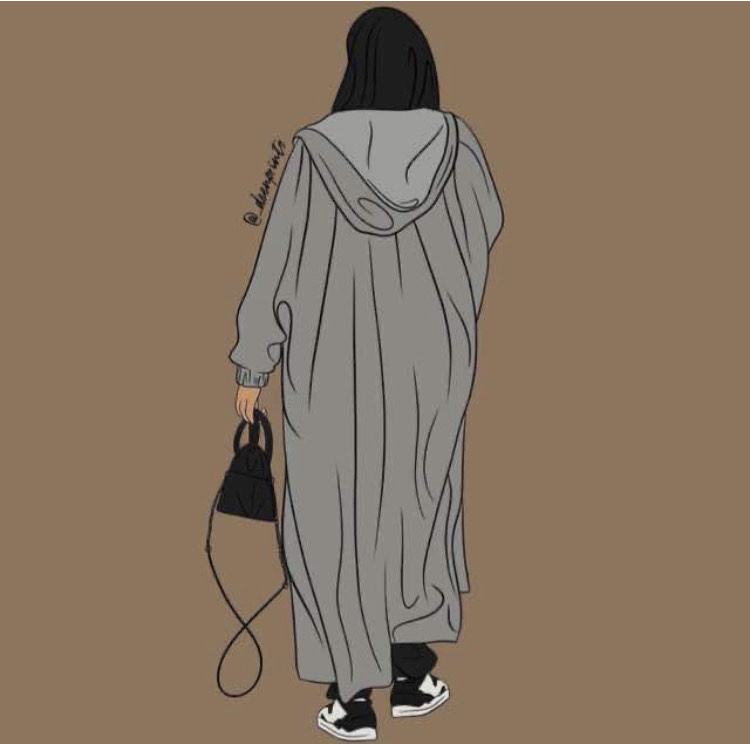
\includegraphics[width=0.23\textwidth]{IMG_4872.jpeg}
\includesvg[width=0.14\textwidth]{anti_CervicalCancer_logo.svg}
\includesvg[width=0.23\textwidth]{Muslim_women_1.svg}
%\includesvg[width=0.14\textwidth]{Muslim_women_2.svg}
%\includesvg[width=0.2\textwidth]{parasite_logo.svg}
\end{center}

\end{frame}
%%%%%%%%%%%%%%%%%%%%%%%%%
\section{Projects}
\begin{frame}
\frametitle{TMM's Projects - first pillar}
% Add content here
\begin{outline}
    TMM is working on a variety of projects to improve healthcare by building capacity, upgrading equipment, implementing screening programs, and collaborating with local health workers and organizations.
    \1 medical affairs
        \2 Providing quality care to patients through referring to the specialists at TMM
        \2 Working on non-communicable diseases (NCD, such as hypertension, diabetes) together with NGOs
        \2 The point-of-care ultrasound in the emergency department and intensive care unit (ICU) of HGH
        \2 On-job-training local physicians to increase their professional expertise, enabling them to provide more systematic and thorough care.
\end{outline}



\end{frame}

\begin{frame}{Medical affairs - trauma ward}
    \begin{center}
        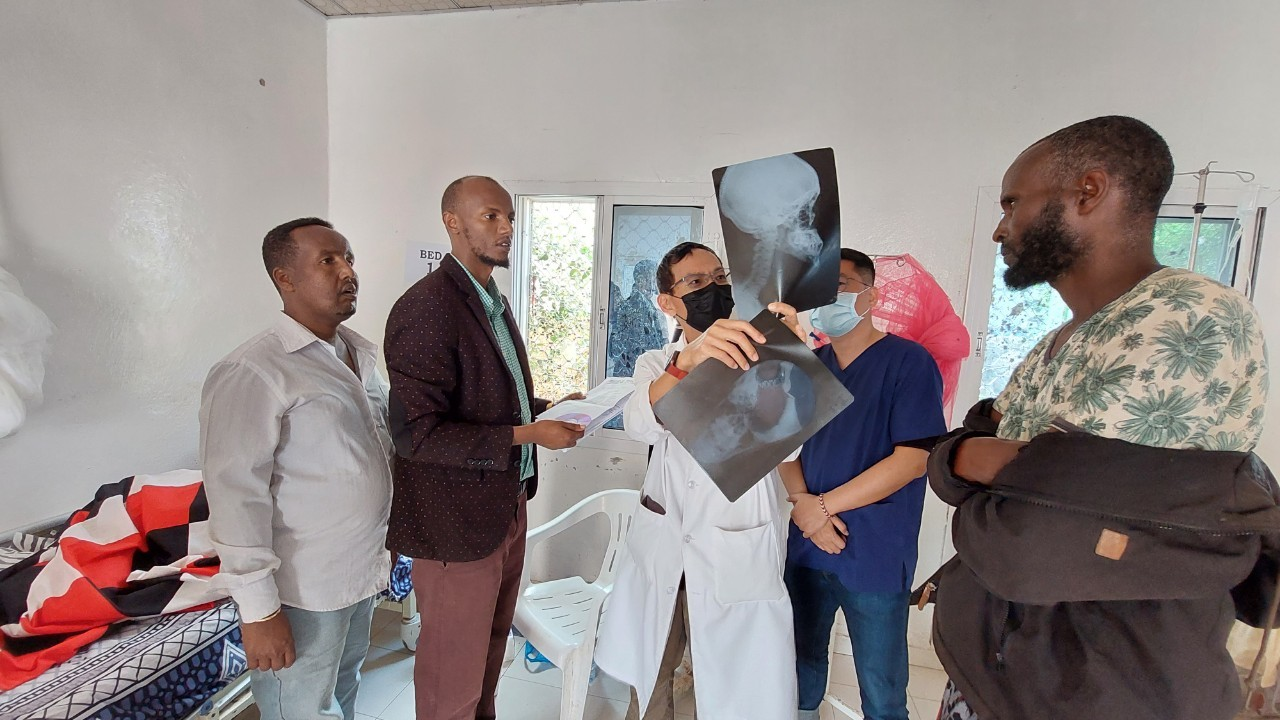
\includegraphics[width=0.8\textwidth]{IMG-4862827583386425169.de8939a35ce768375740b709dce51958.23032108.JPG}
%        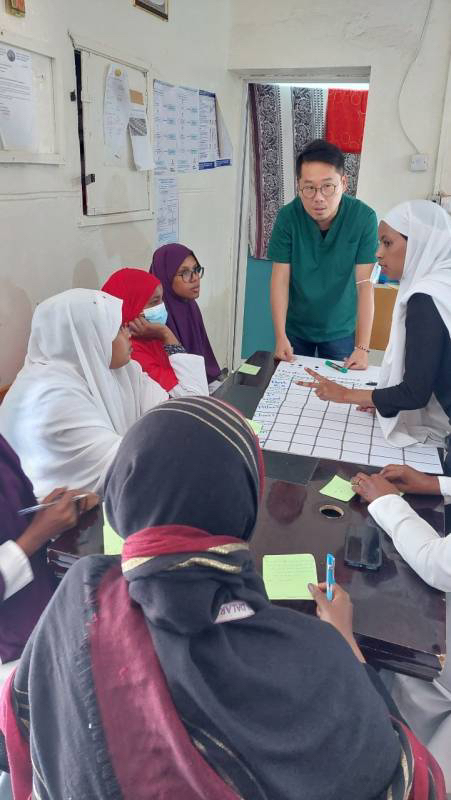
\includegraphics[width=0.2\textwidth]{6963.jpg}
    \end{center}
\end{frame}
    
\begin{frame}{Medical affairs - operation theatre}
    \begin{center}
        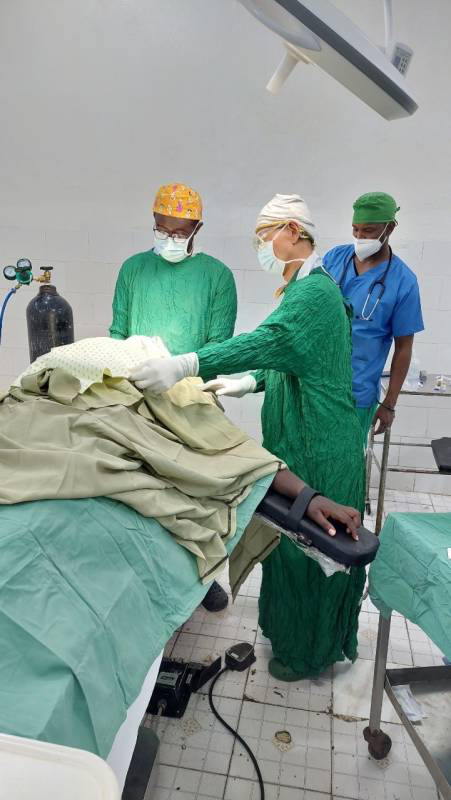
\includegraphics[width=0.35\textwidth]{51744_old_table.jpg}
%        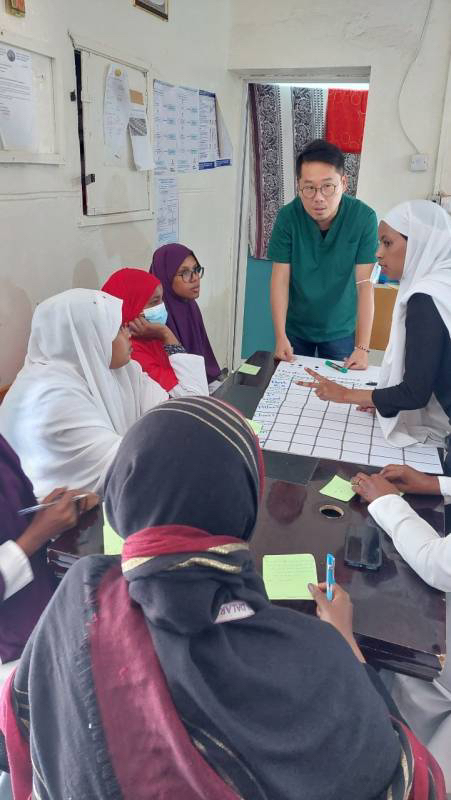
\includegraphics[width=0.2\textwidth]{6963.jpg}
    \end{center}
\end{frame}


\begin{frame}{Medical affairs - OBS, ED}
    \begin{center}
        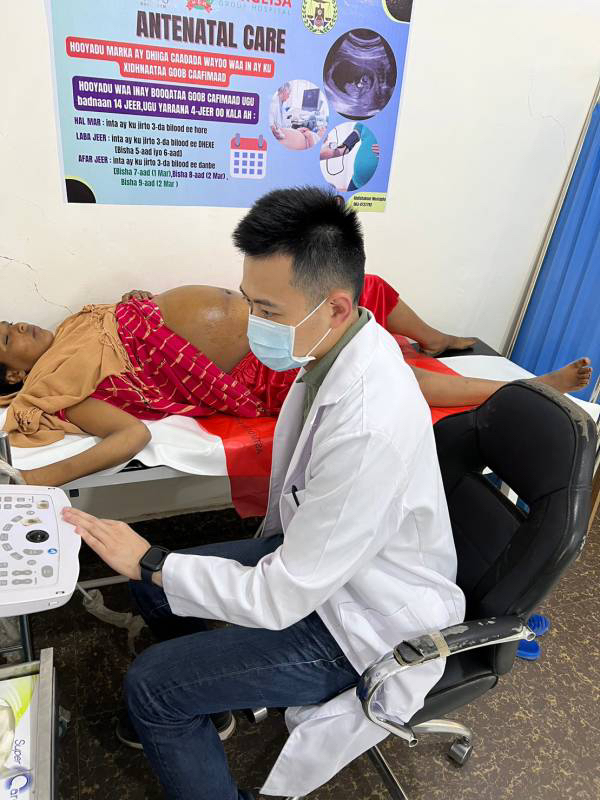
\includegraphics[width=0.25\textwidth, trim=50mm 20mm 40mm 50mm, clip]{52165_antenatal_check.jpg}
        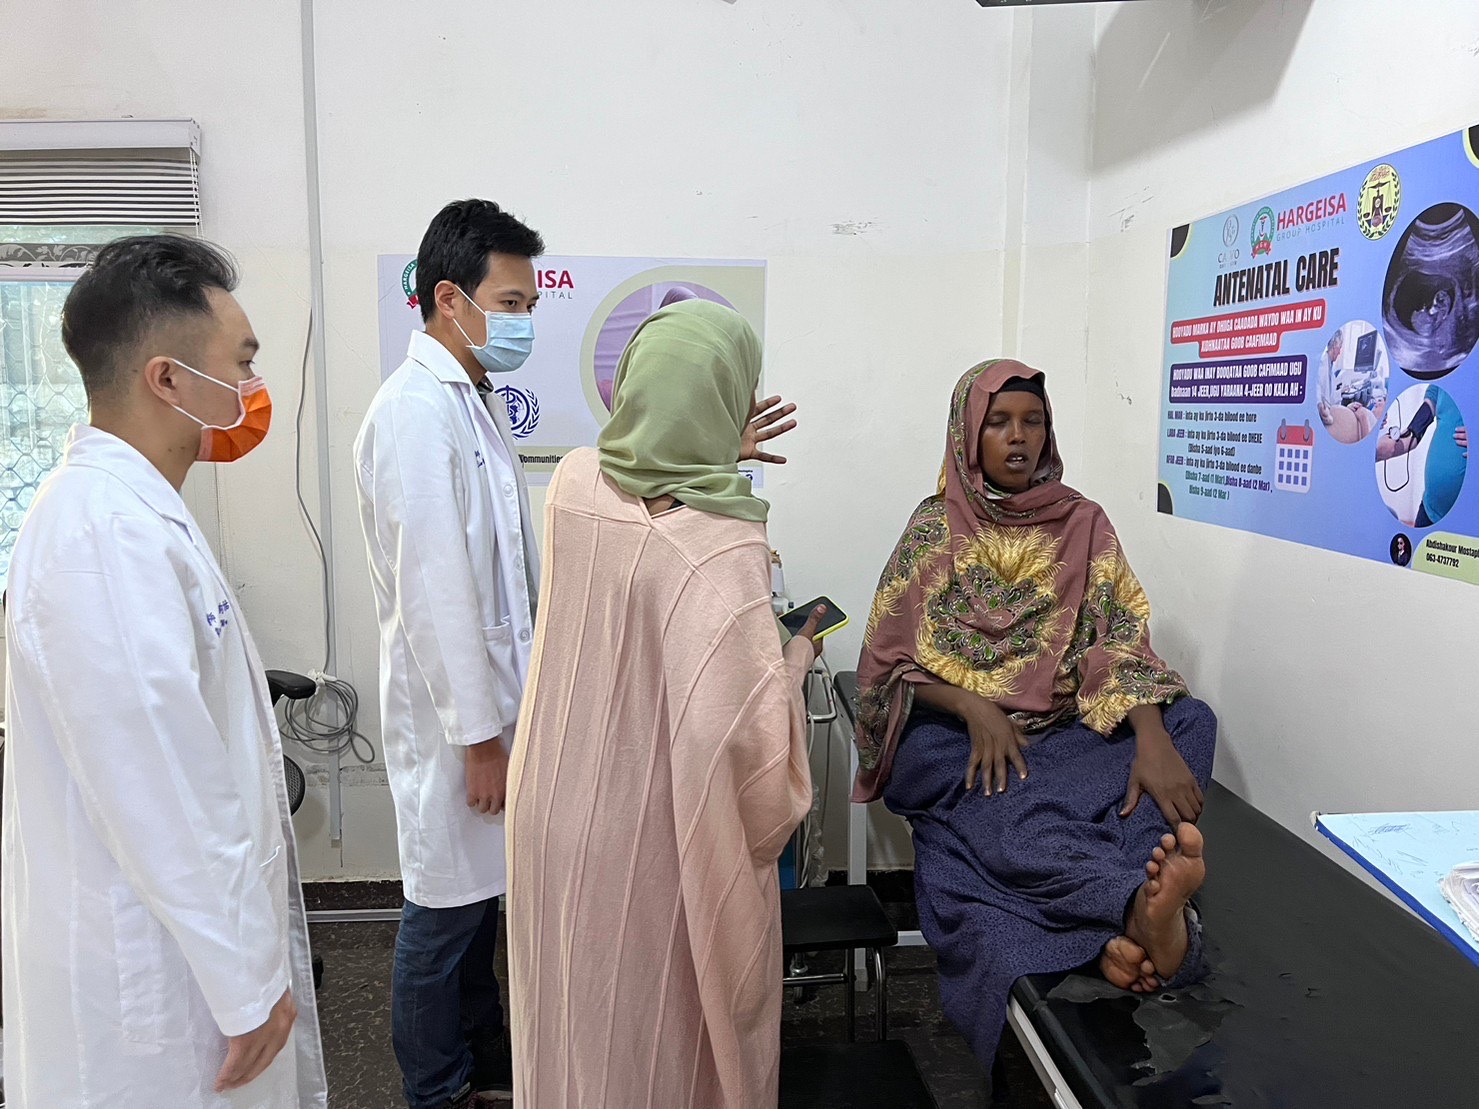
\includegraphics[width=0.4\textwidth]{IMG_5068.jpeg}
    \end{center}
\end{frame}

\begin{frame}{Medical affairs - ED, ward}
\begin{center}
\begin{tikzpicture}
    \node[anchor=south west,inner sep=0] (image) at ($(current page.center)+(0cm,-2cm)$) {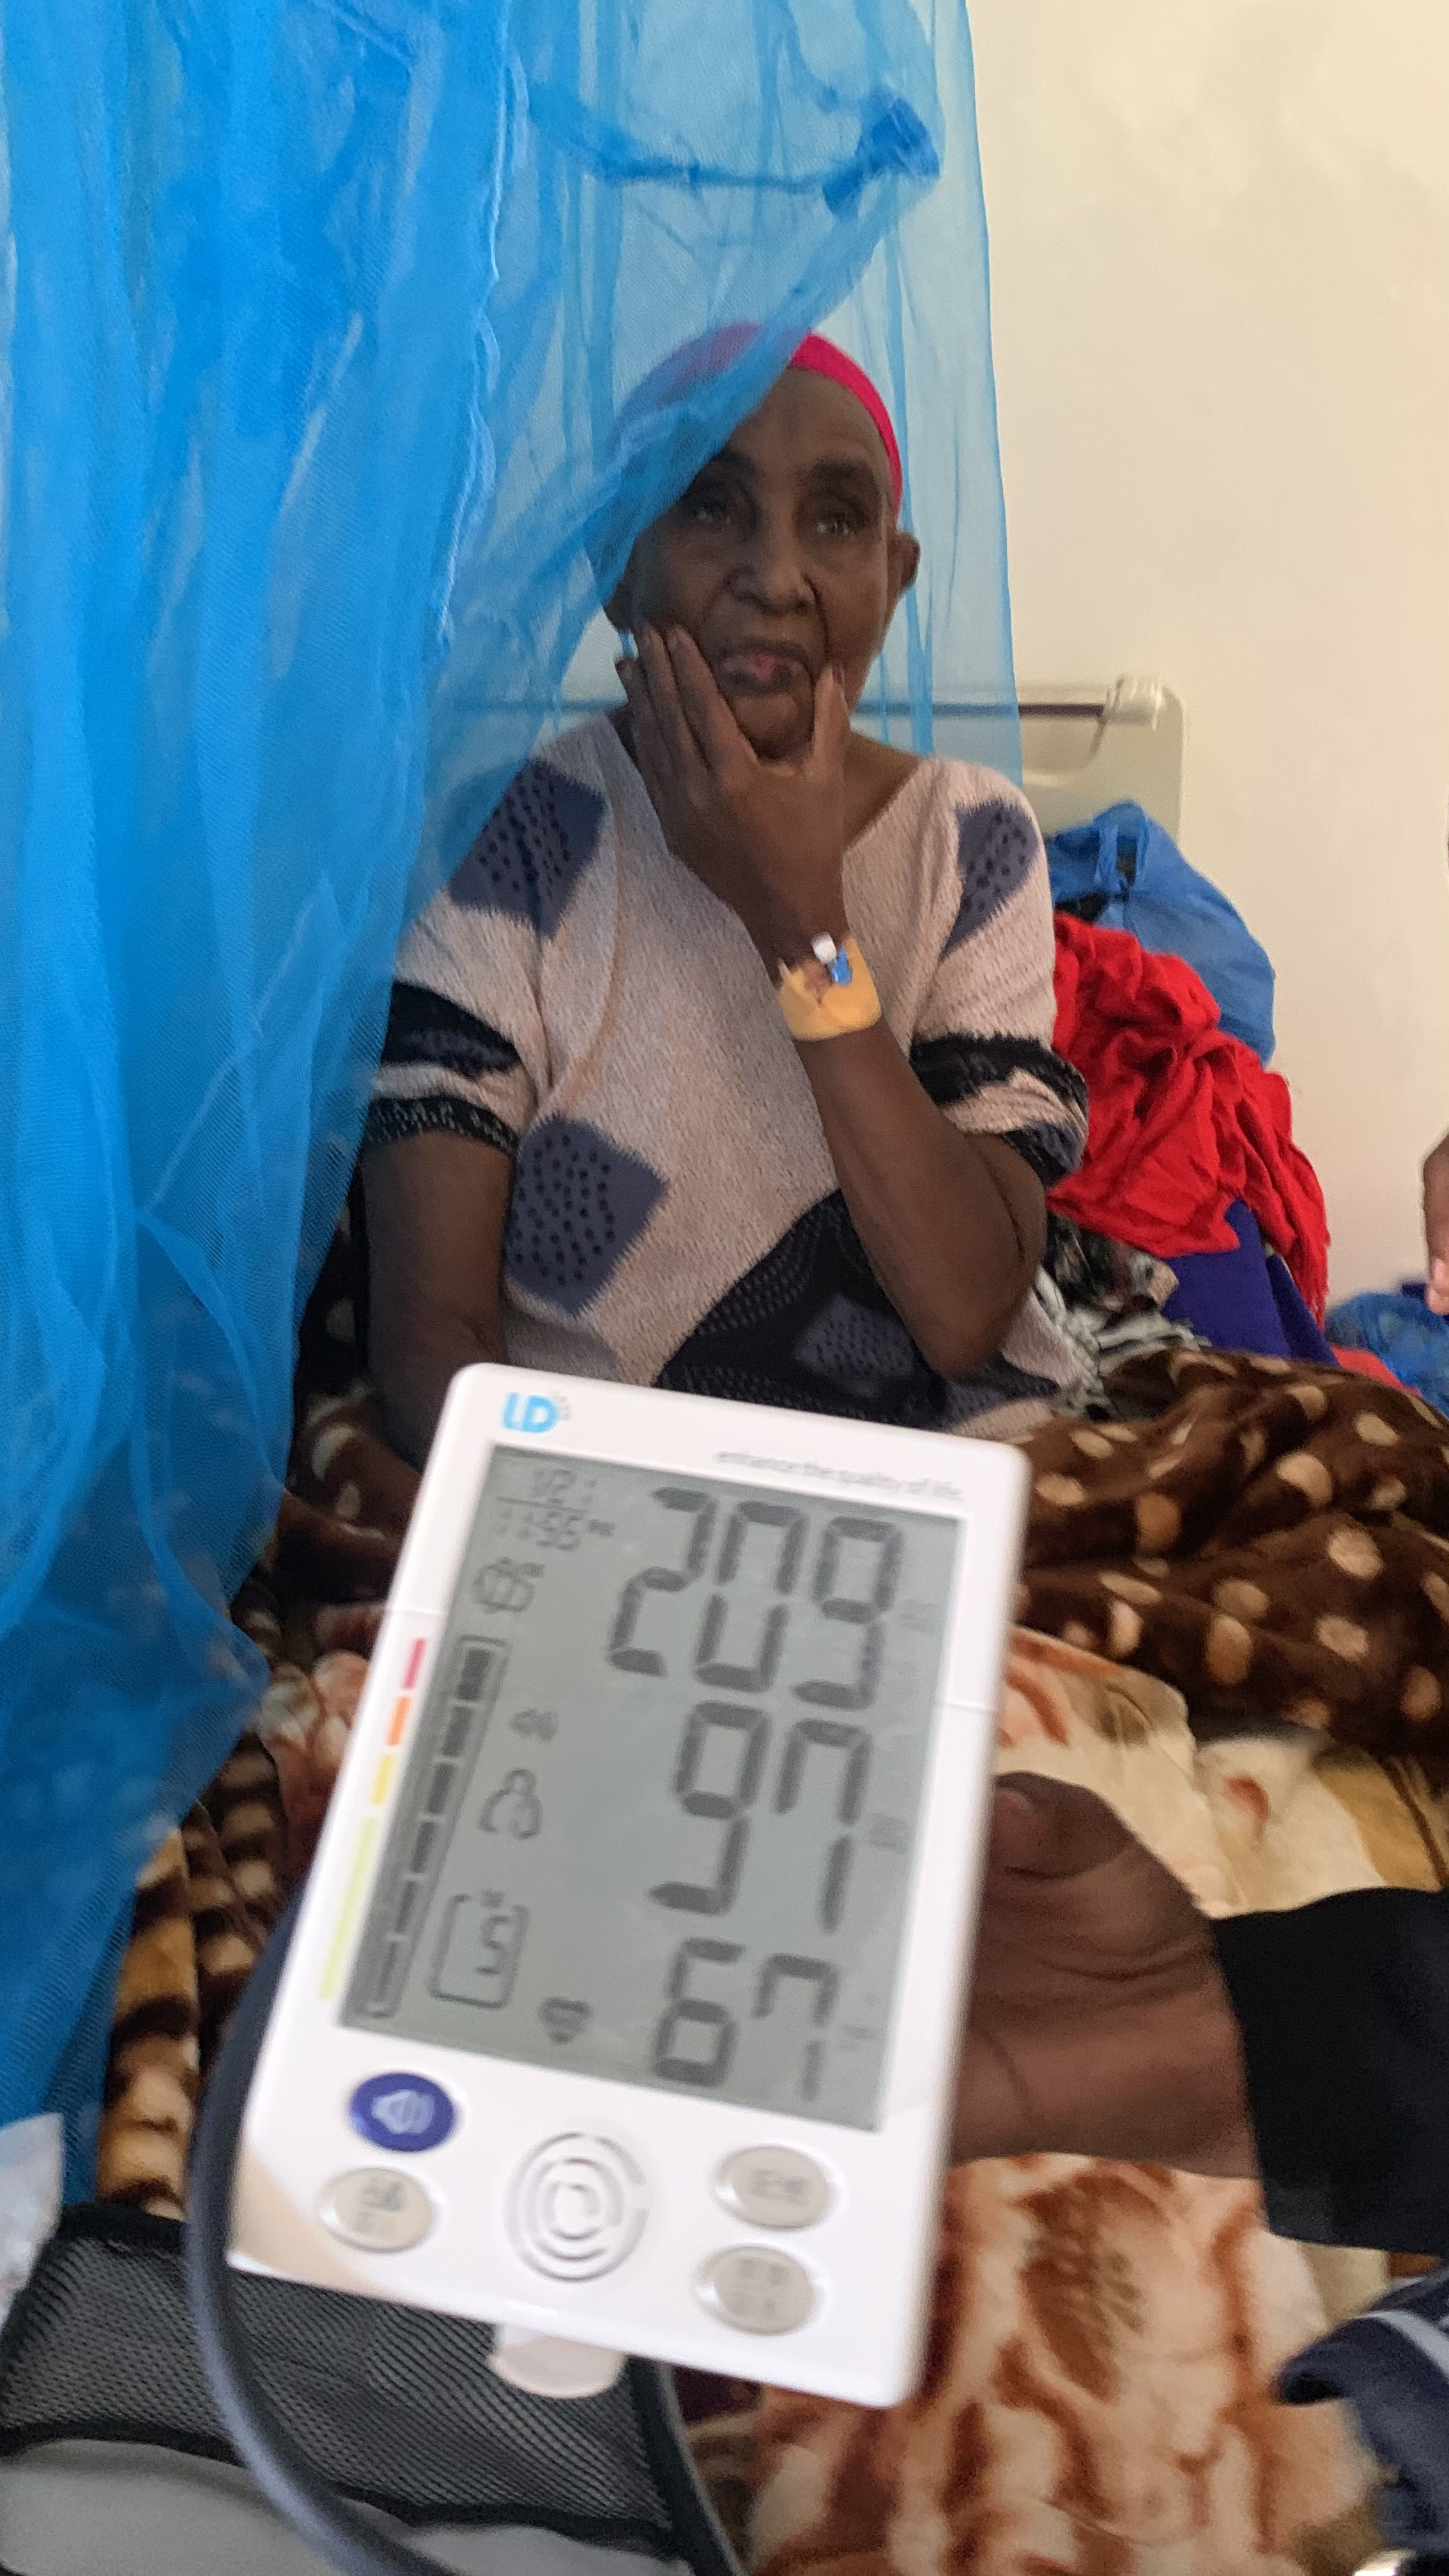
\includegraphics[width=0.30\textwidth]{IMG_5011.jpeg}};
    \begin{scope}[x={(image.south east)},y={(image.north west)}]
        \fill[white] (0.35,0.75) circle (0.03);
    \end{scope}
\end{tikzpicture}

\end{center}
\end{frame}


\begin{frame}{Home visits - OBS, ED}
    \begin{center}
        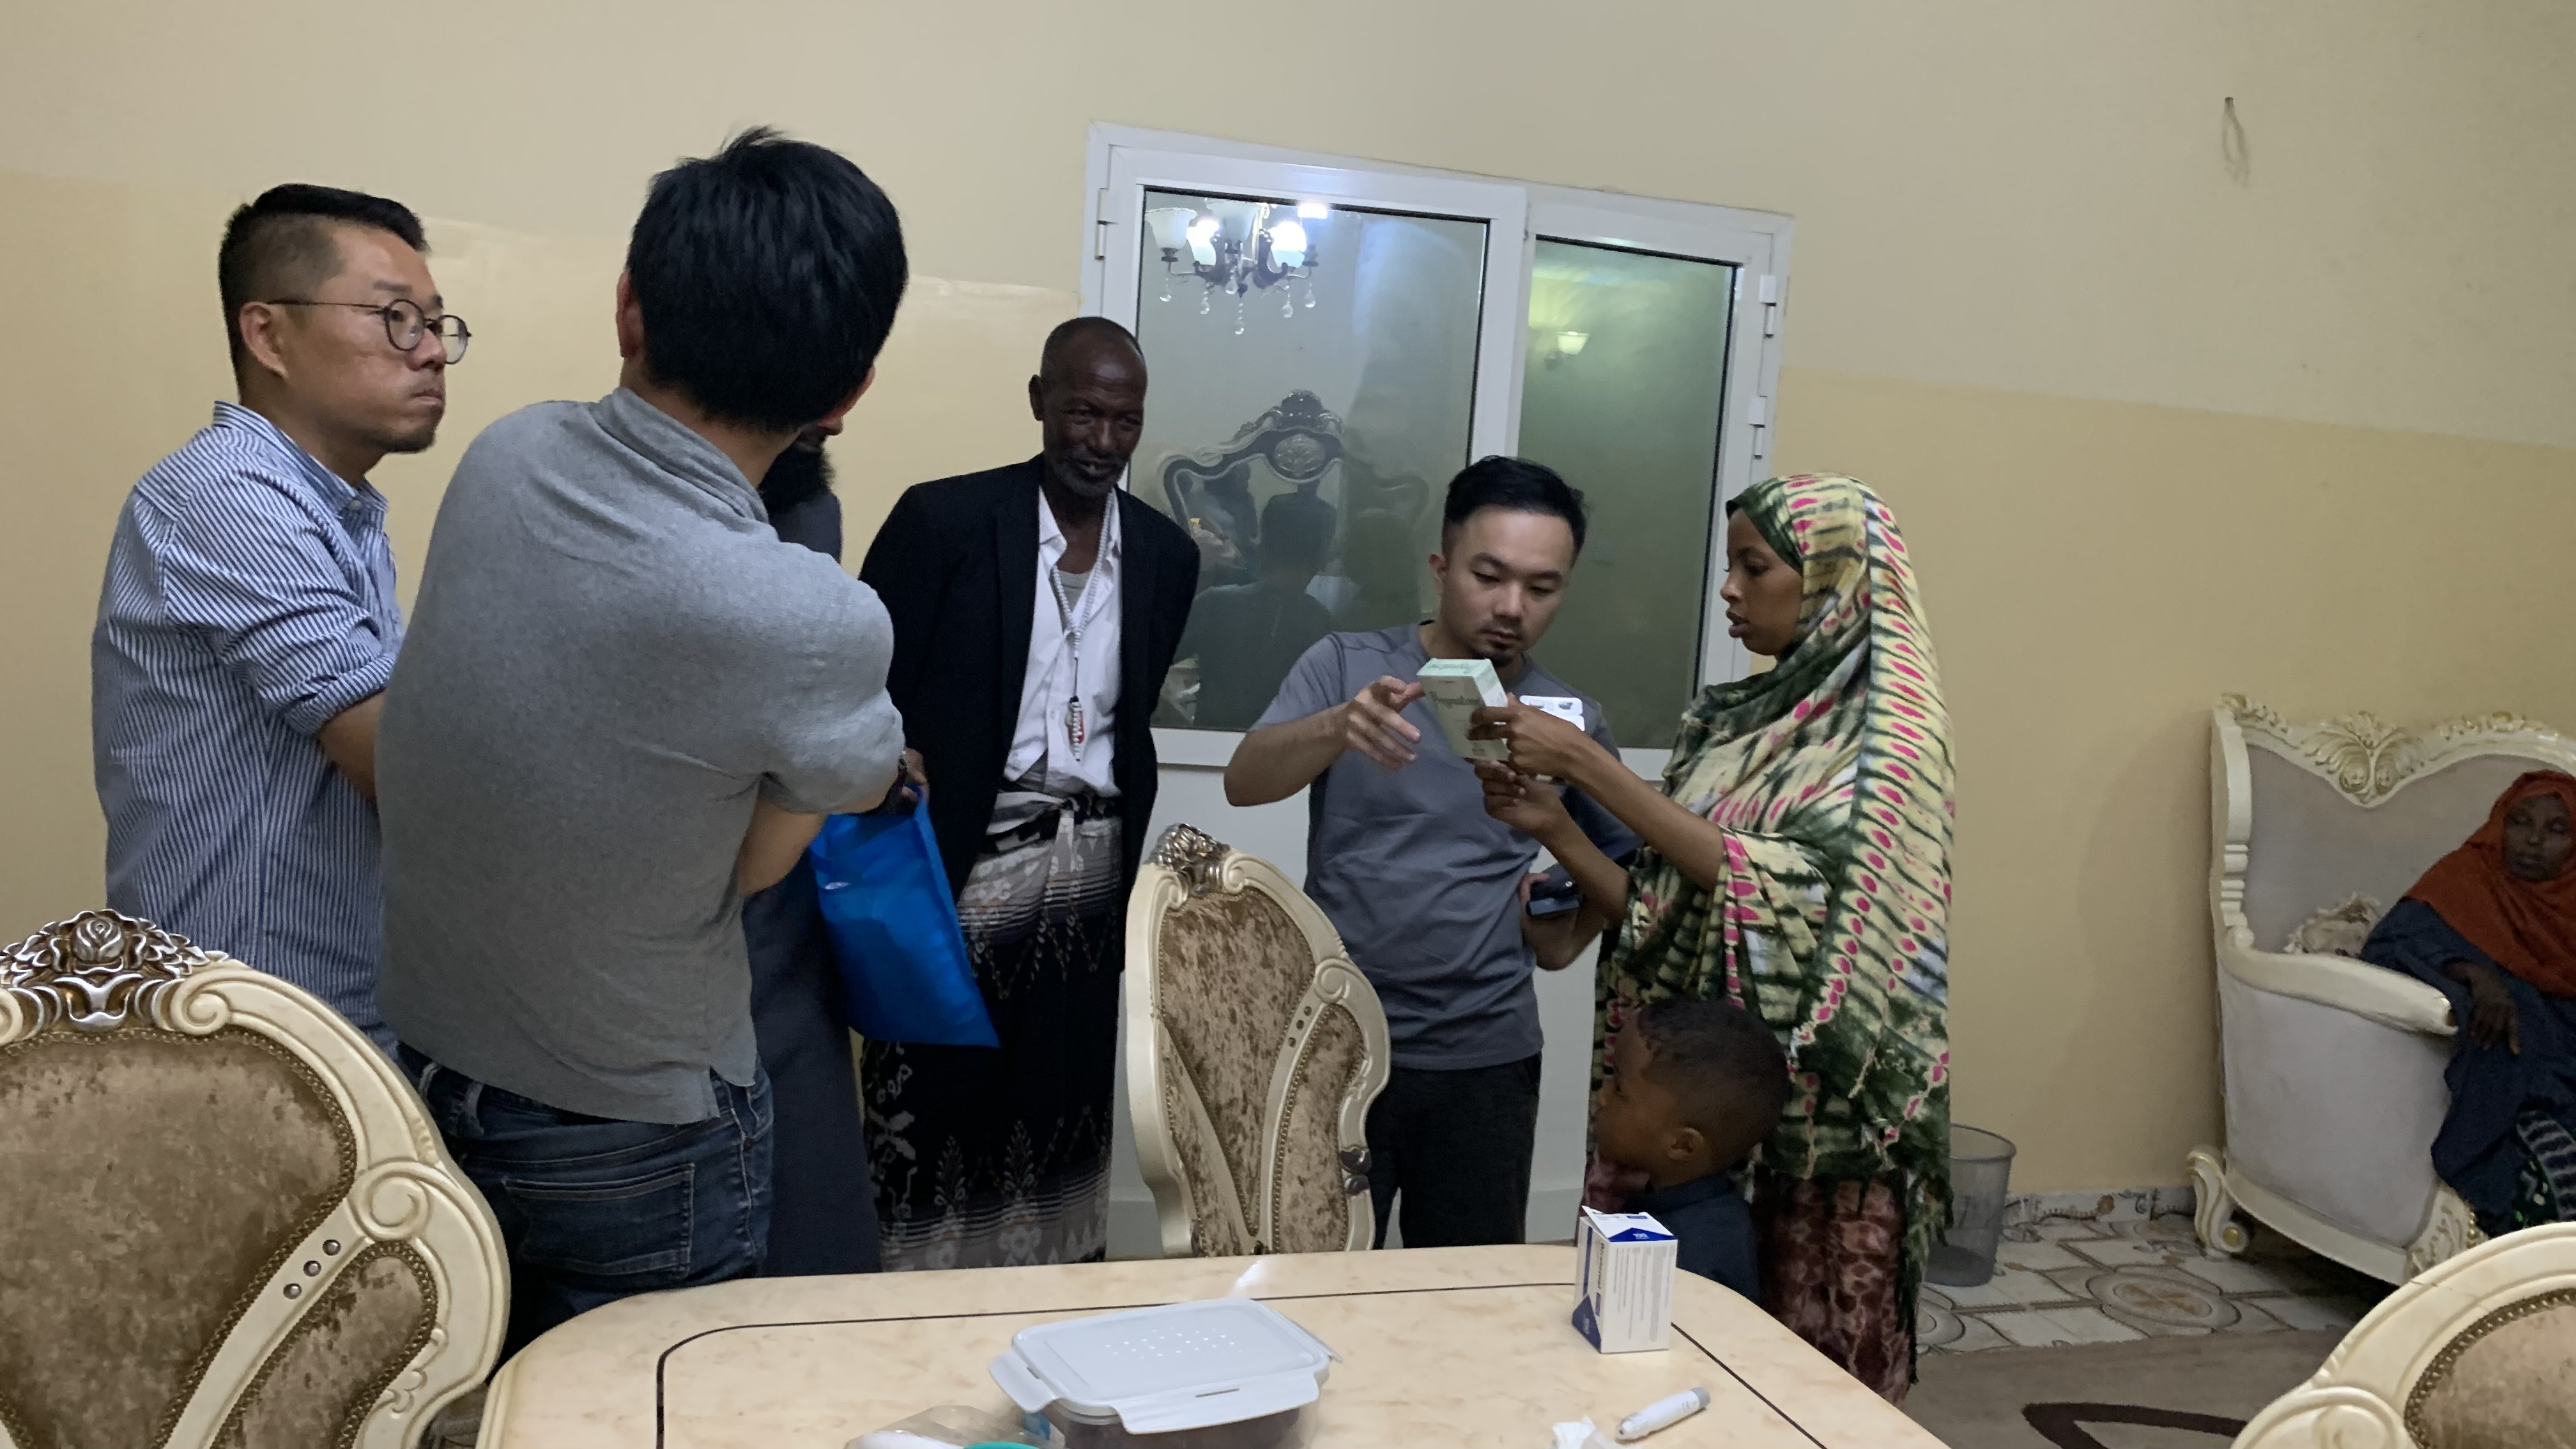
\includegraphics[width=0.55\textwidth]{IMG-5075.jpg}
        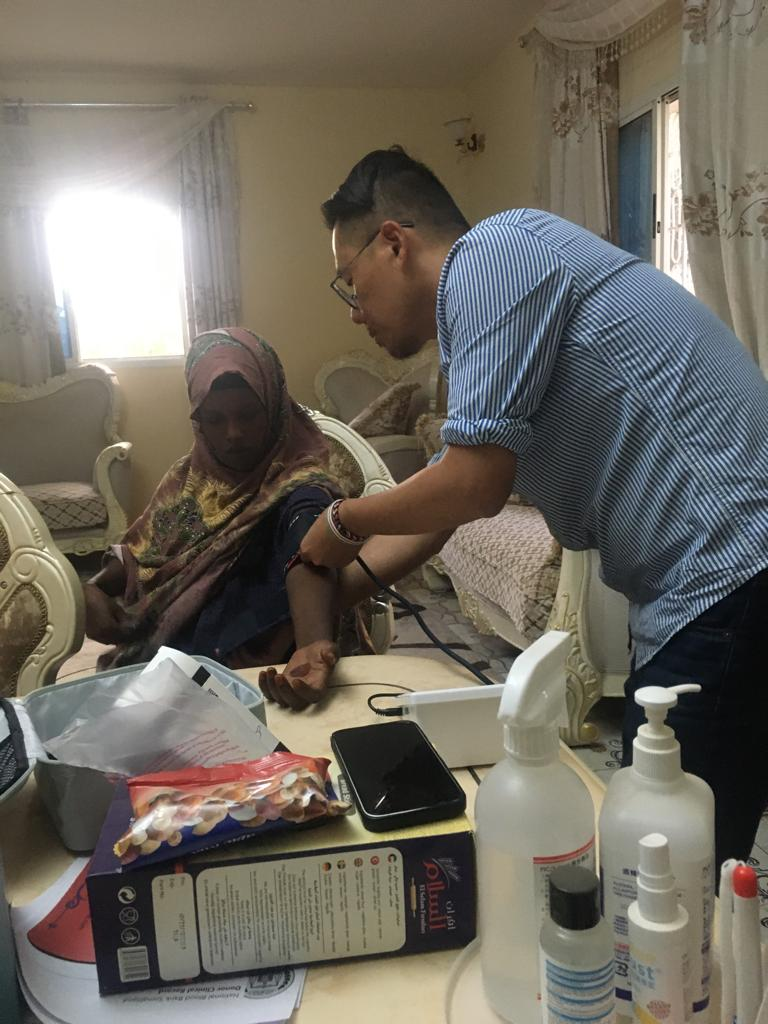
\includegraphics[width=0.25\textwidth]{386eb640-9657-4b71-af5c-5de19cb7b159.JPG}
    \end{center}
\end{frame}


\begin{frame}{Home visits - OMS}
    \begin{center}
        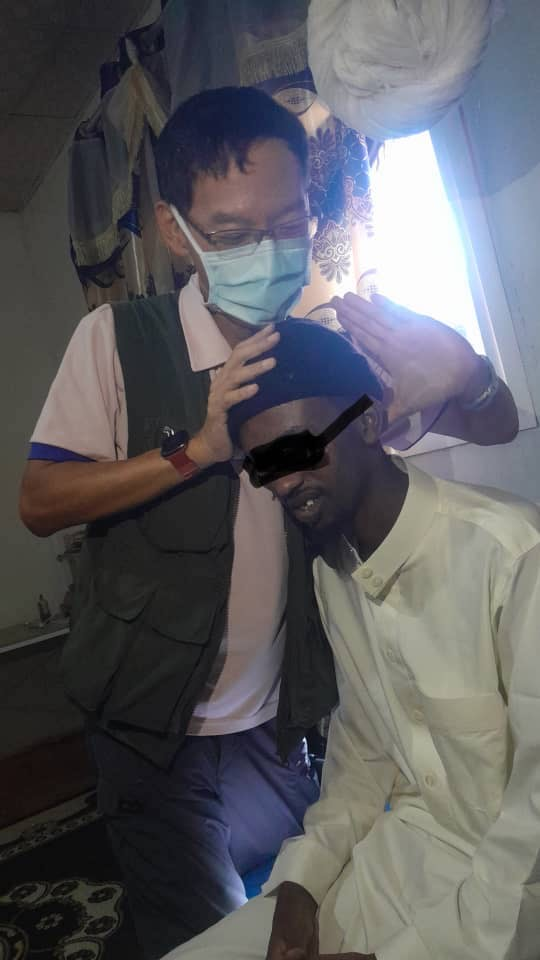
\includegraphics[width=0.20\textwidth]{399223ed-f871-41f7-ae57-c90a5f0ee459.jpeg}
        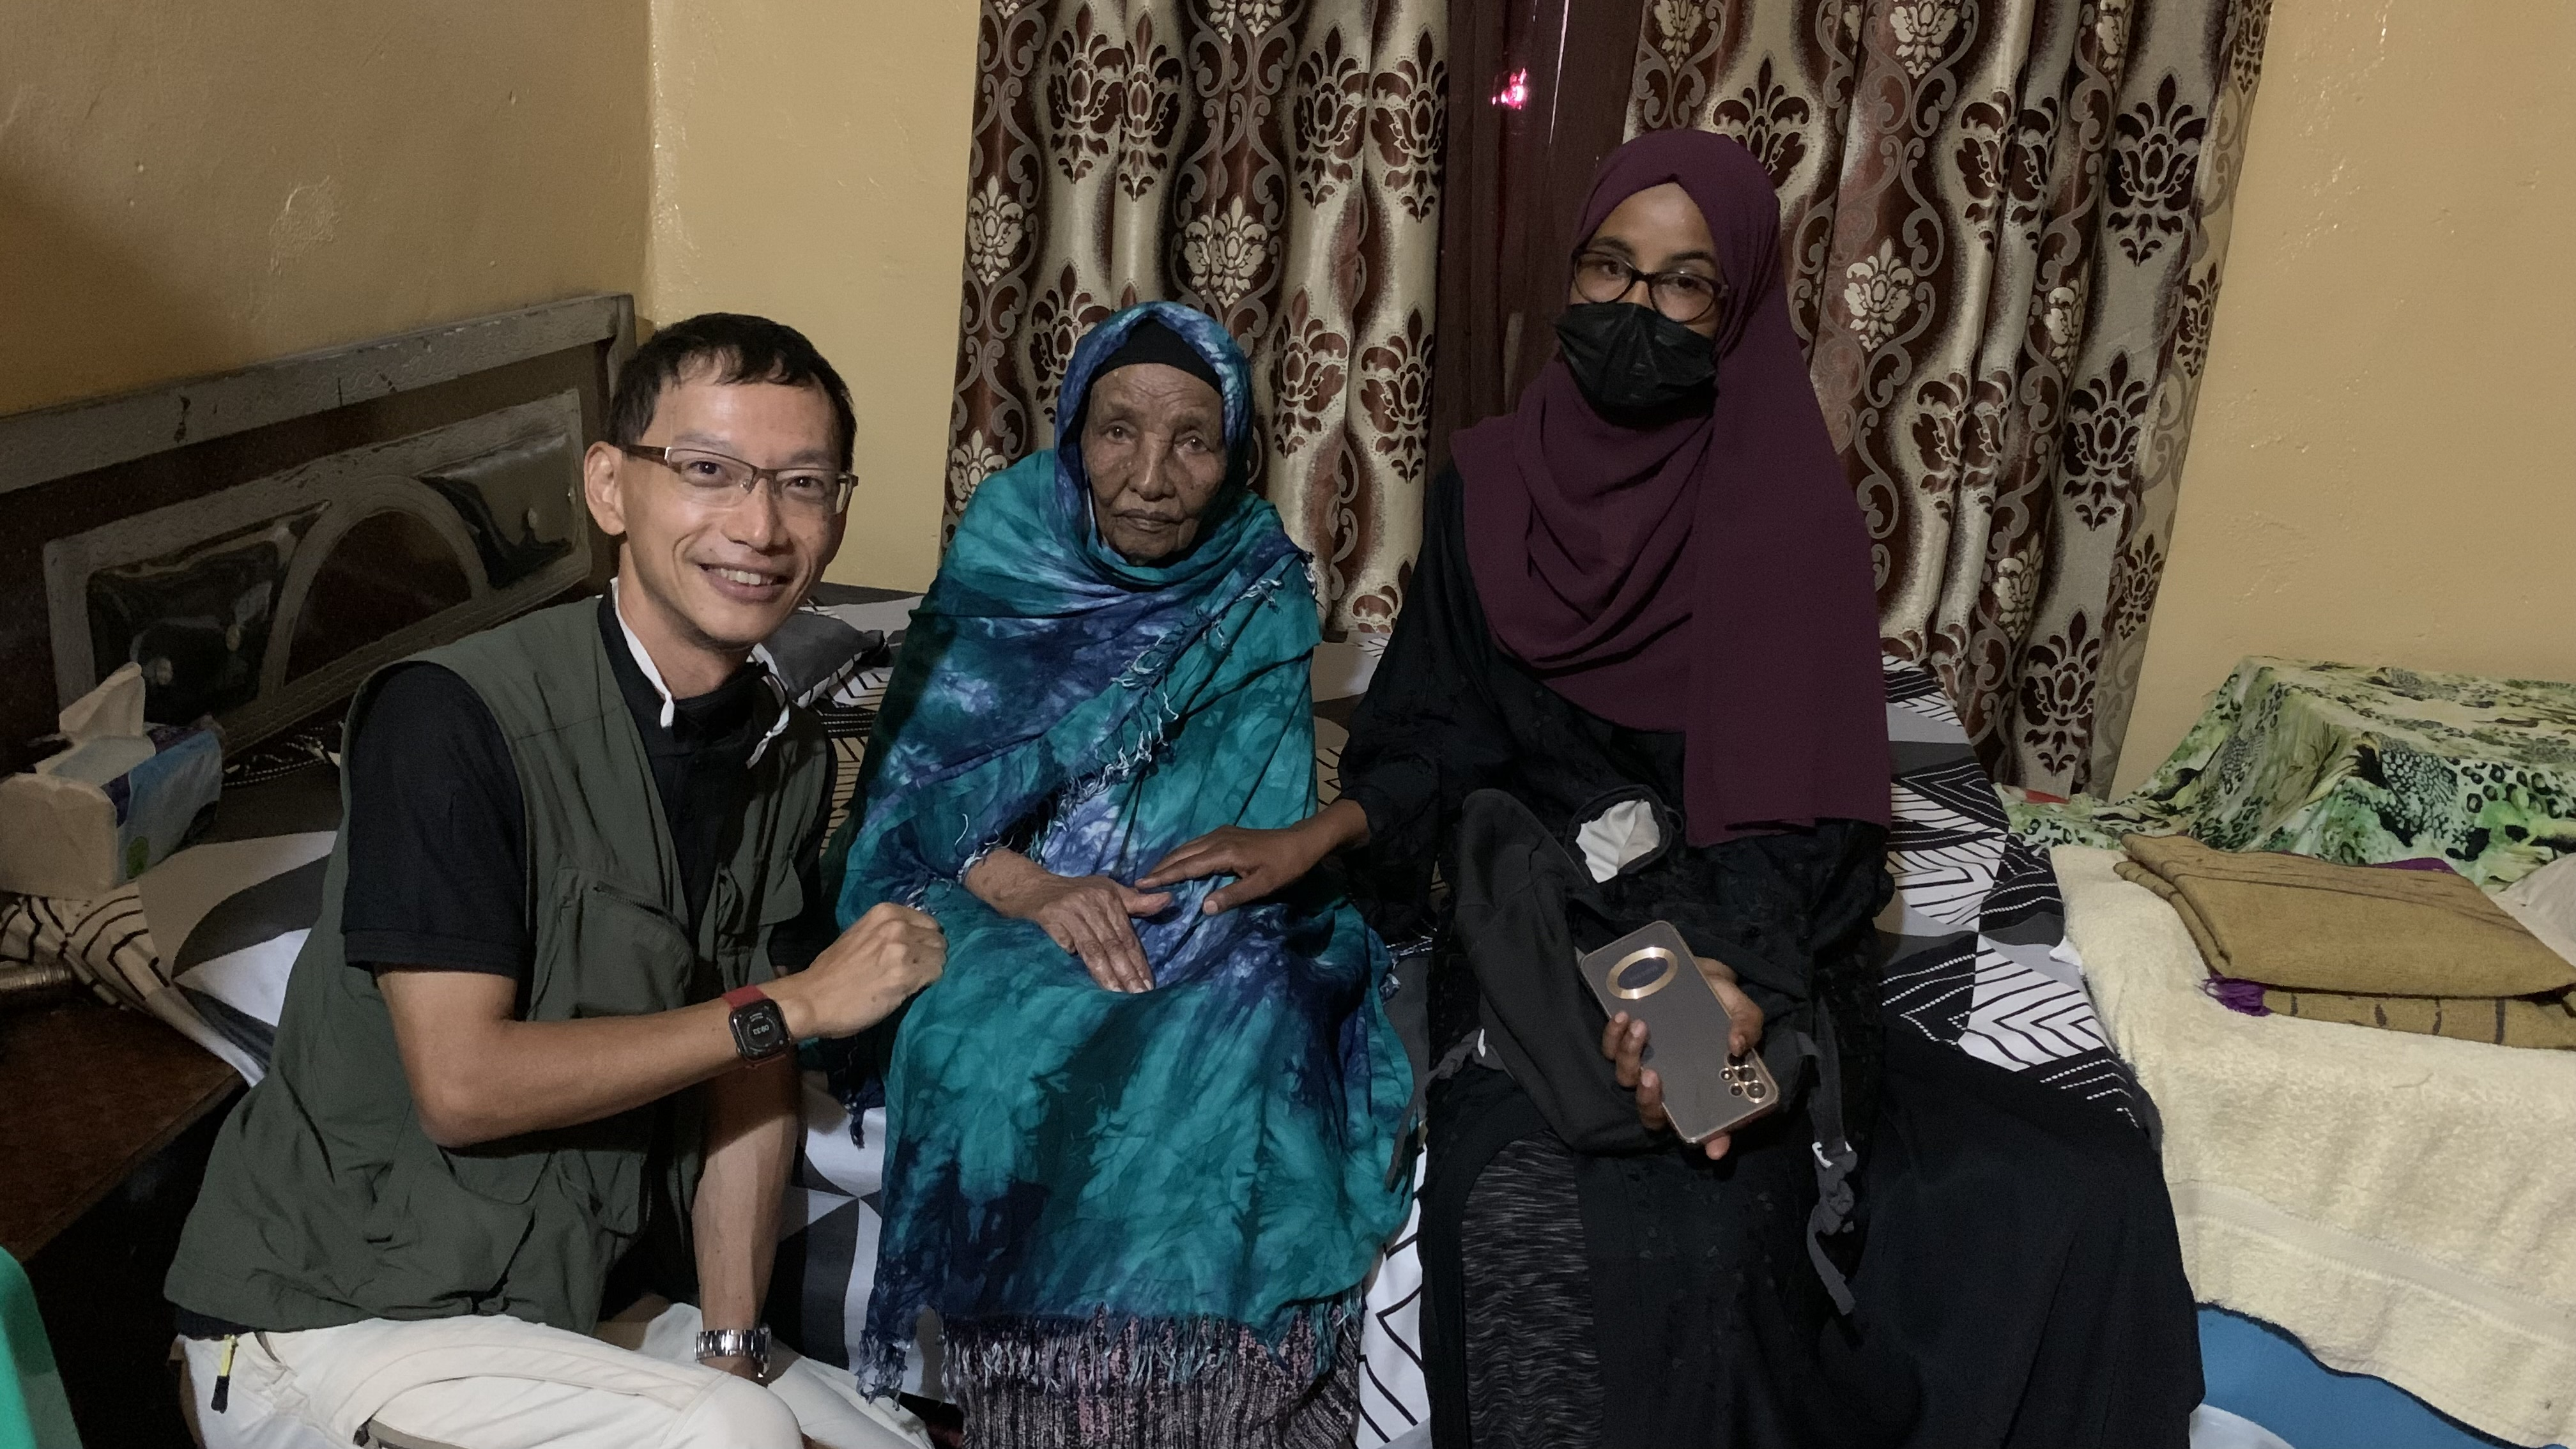
\includegraphics[width=0.50\textwidth]{IMG-3330.jpg}
    \end{center}
\end{frame}




\begin{frame}{Home visits - doctor becomes patient}
    \begin{center}
        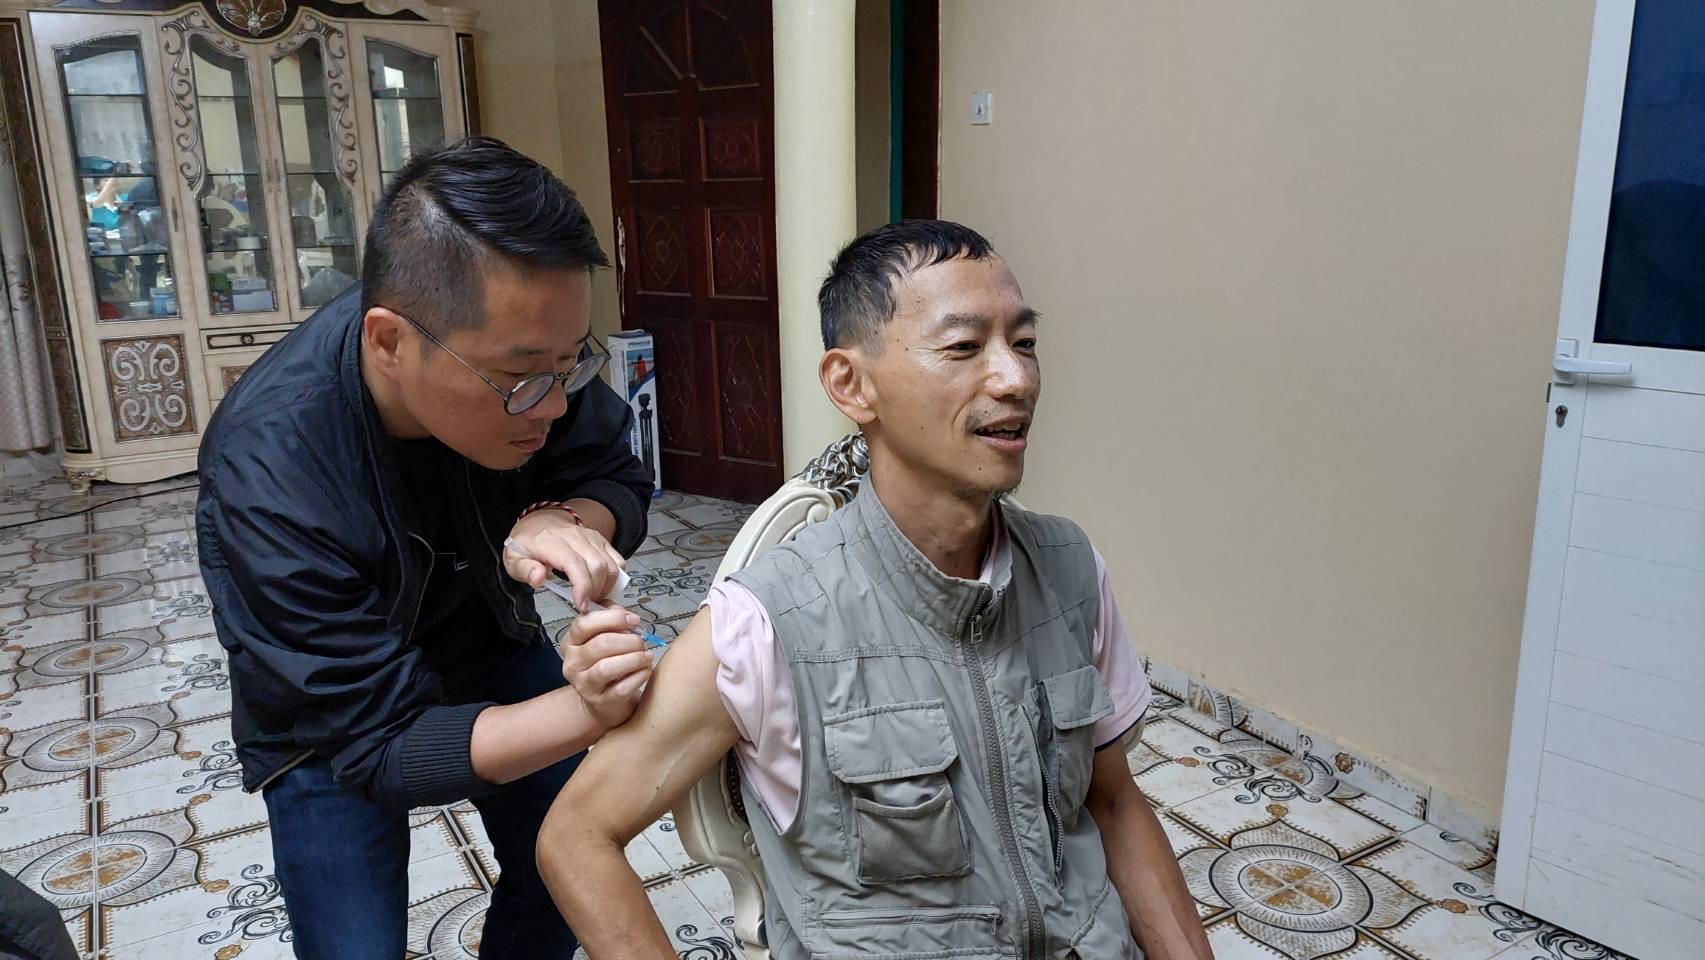
\includegraphics[width=0.50\textwidth]{IMG-2343.JPG}
        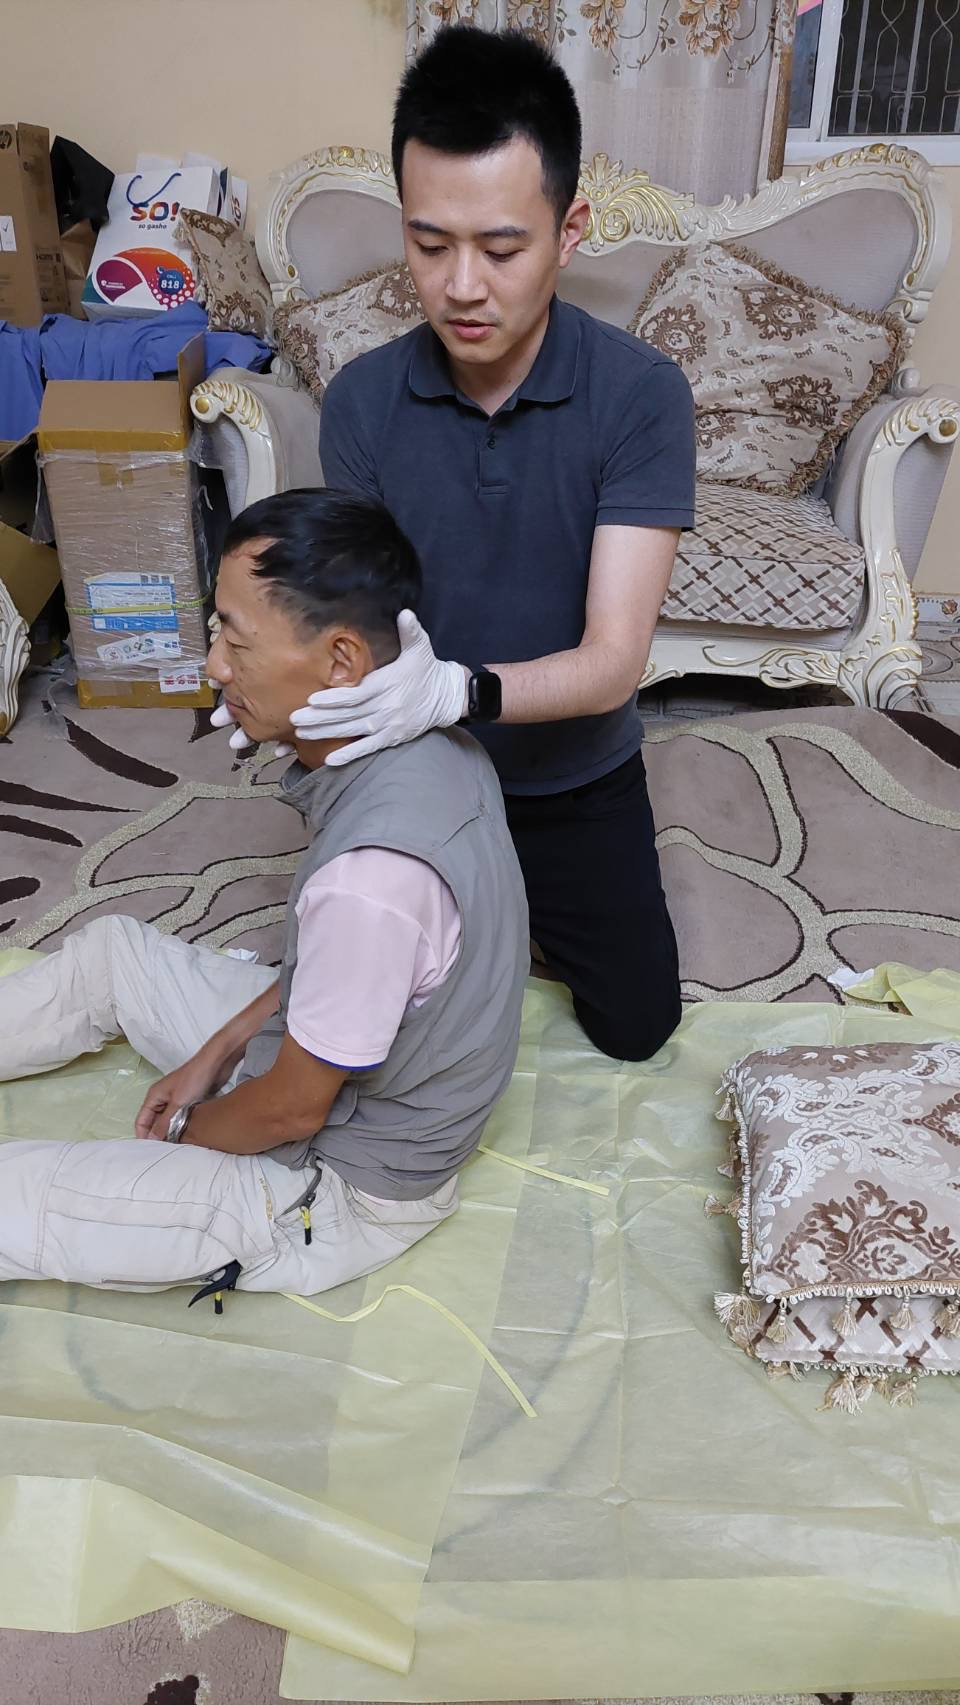
\includegraphics[width=0.20\textwidth]{IMG-2338.JPG}
    \end{center}
\end{frame}

%%%%
\begin{frame}
\frametitle{TMM's Projects - second pillar}
% Add content here
\begin{outline}    
    \1 capacity building
        \2 Contributing to system and equipment upgrades in the orthopedic ward

        \2 In operation theatre (OT), supporting video intubation system, surgical tables, C-arm X-ray, arthroscopic shaver, orthopedic instruments/implants, and other medical devices and medicines for use in HGH
        \2 Instructing interns at the University of Hargeisa (UoH)
        \2 Teaching nurses critical thinking skills

        \2 Building trauma kits for Somaliland army force
        \2 Assist in establishing department of urology in HGH and their resident training program
\end{outline}
\end{frame}

\begin{frame}{Capacity building: orthopedic}
    \begin{center}i
        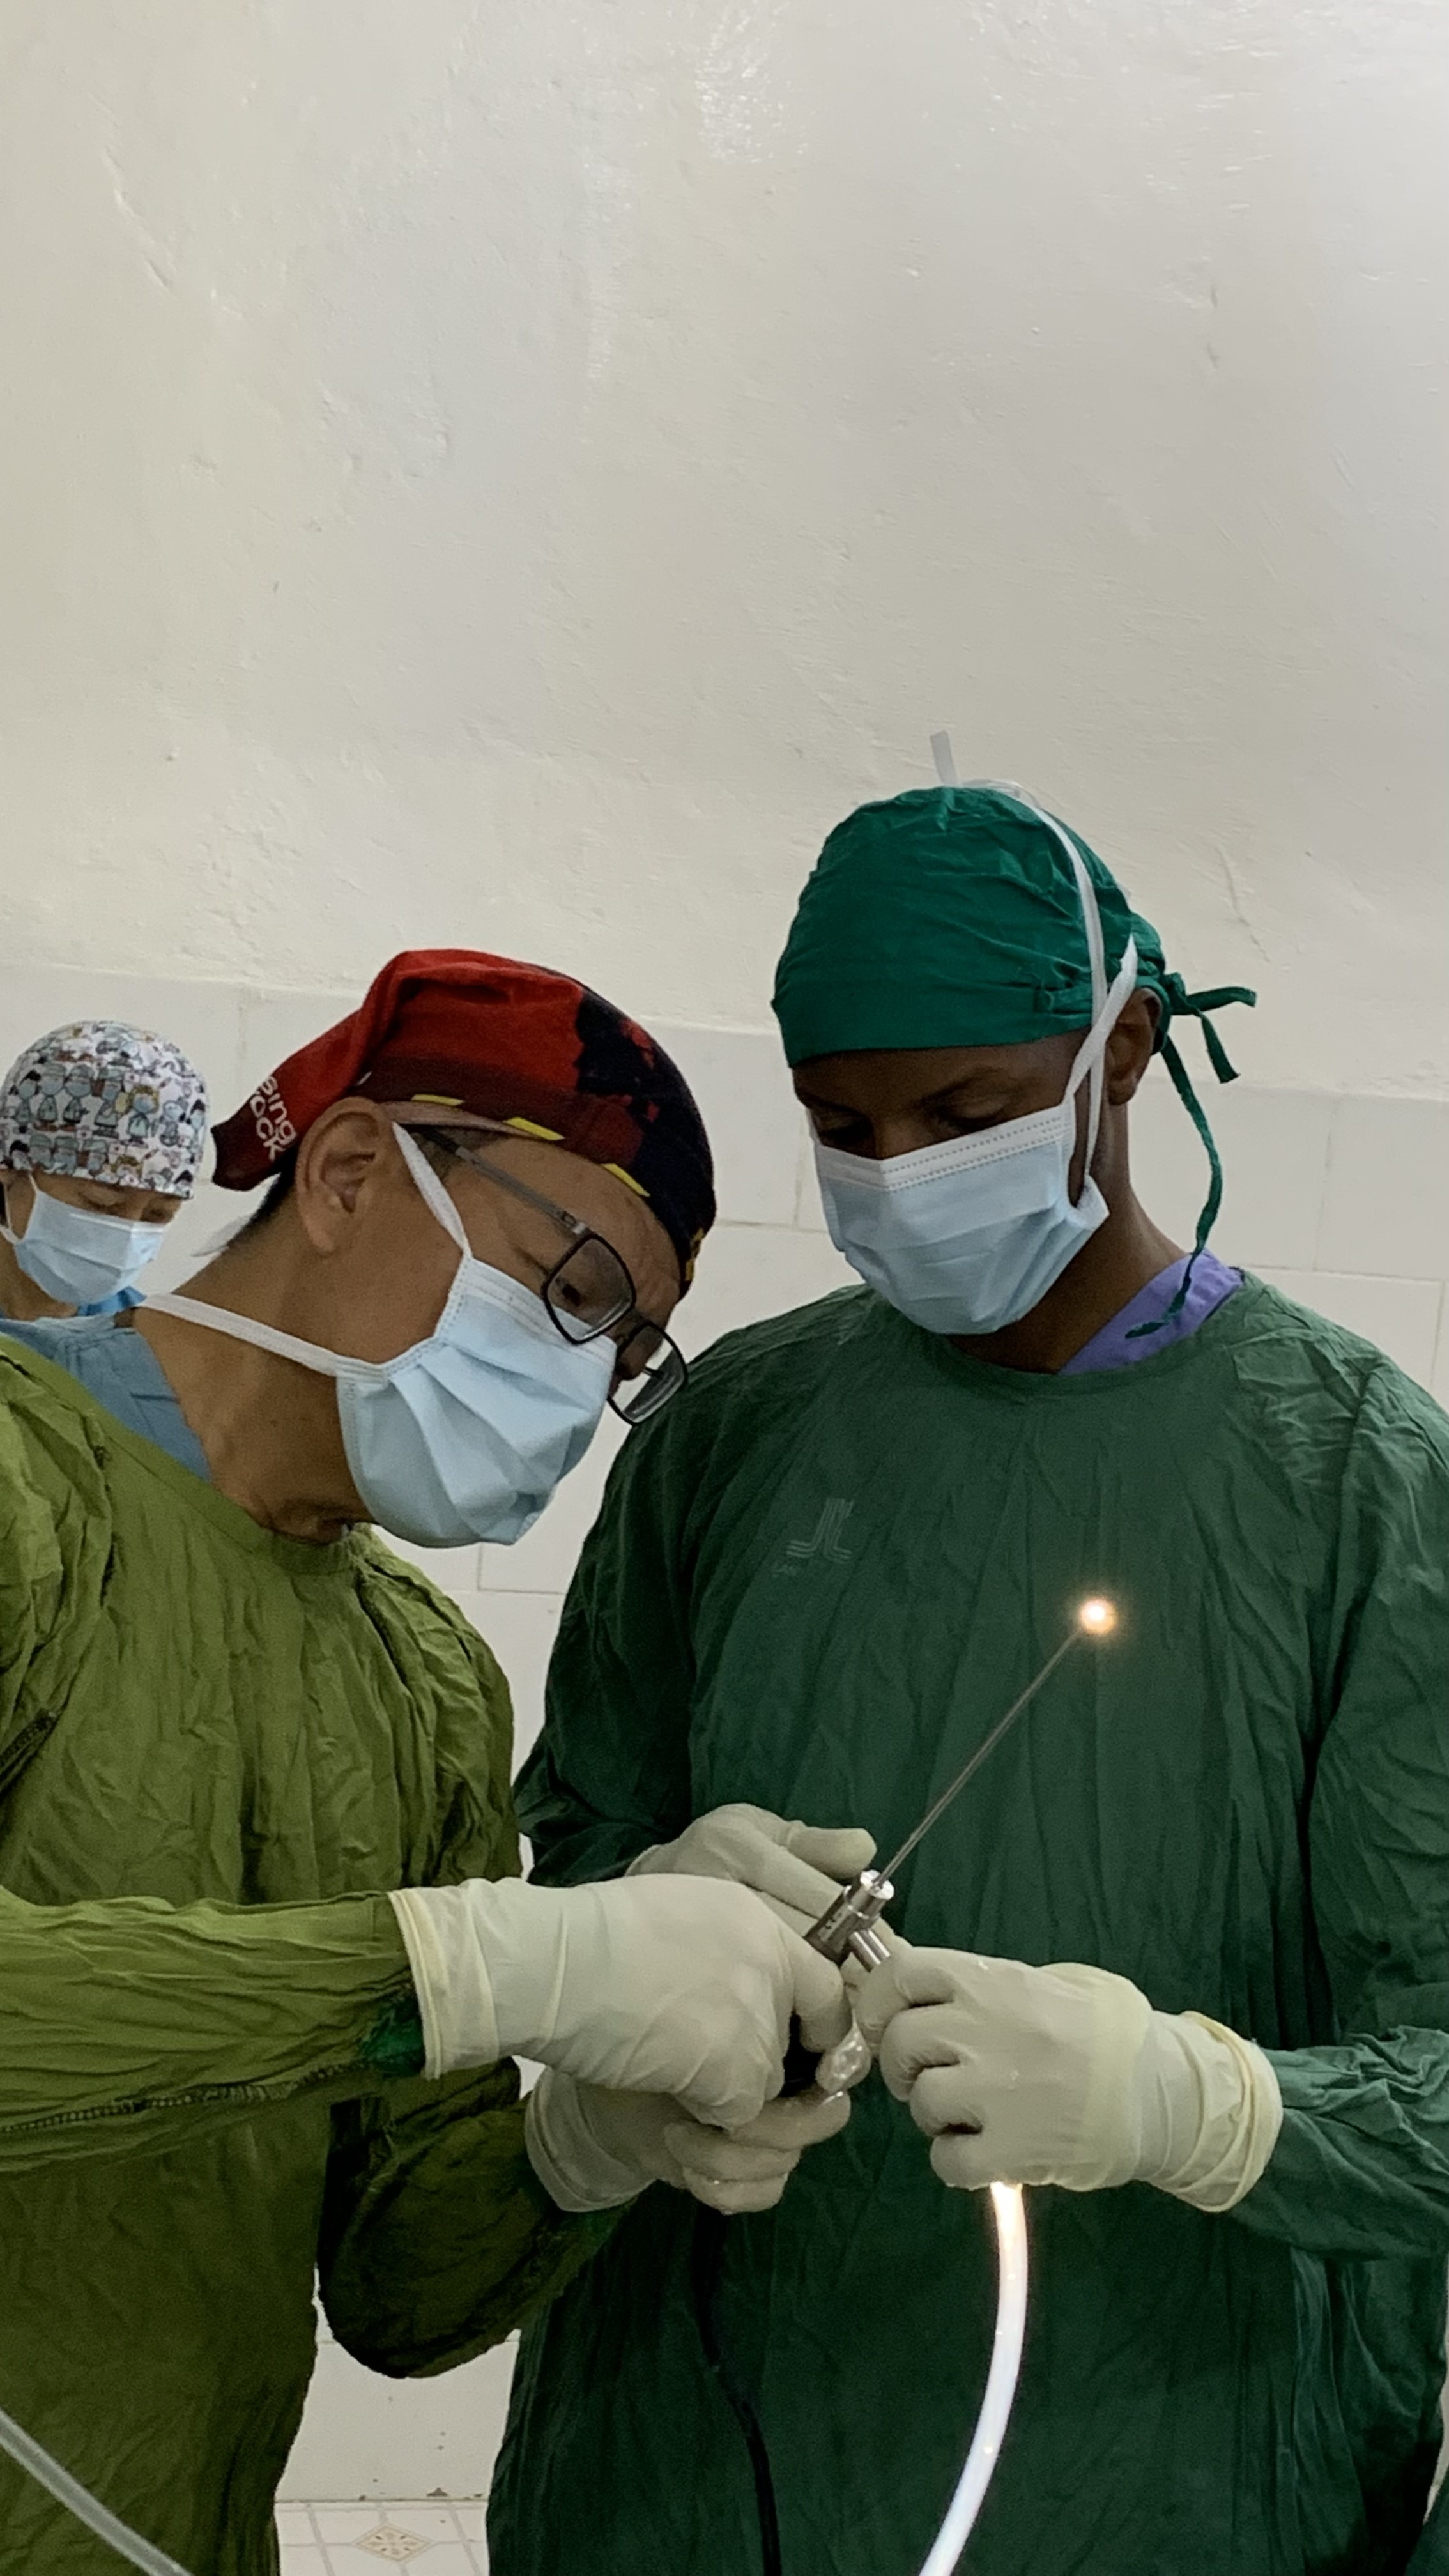
\includegraphics[width=0.30\textwidth]{IMG-6067.jpg}
        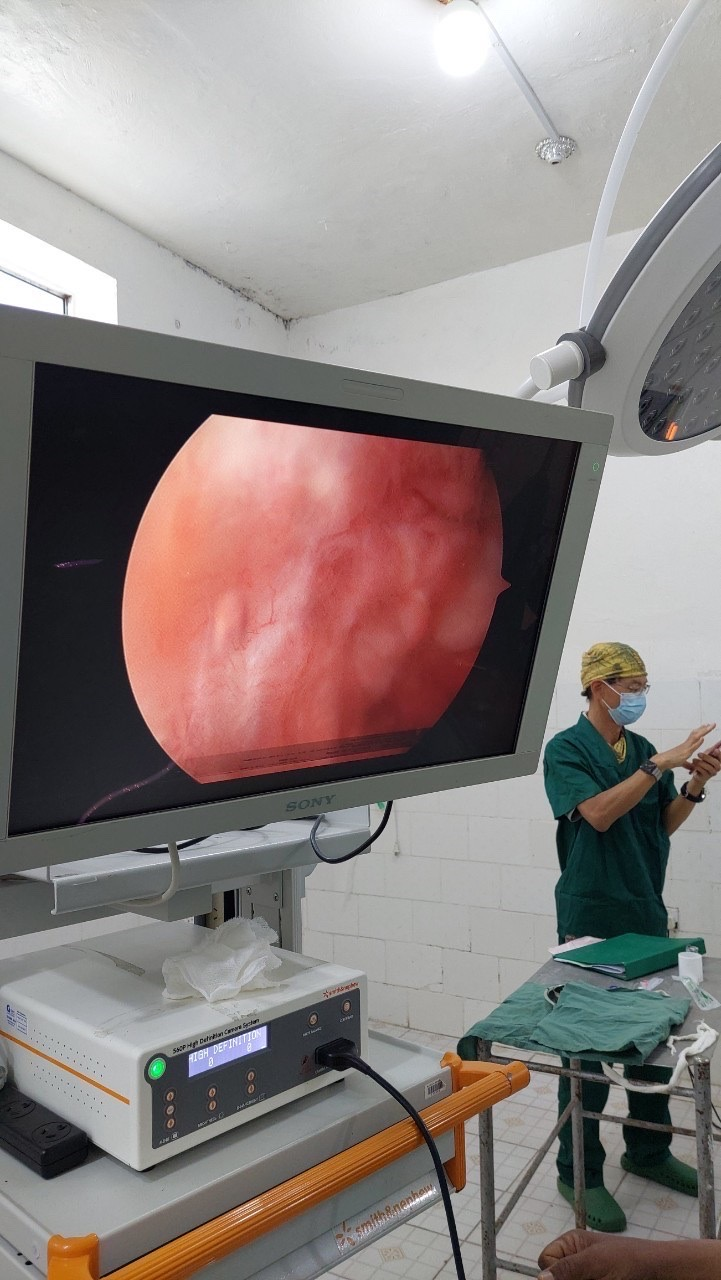
\includegraphics[width=0.30\textwidth]{IMG-6227.JPG}
    \end{center}
\end{frame}


\begin{frame}{Capacity building: nurse, urology}
    \begin{center}
        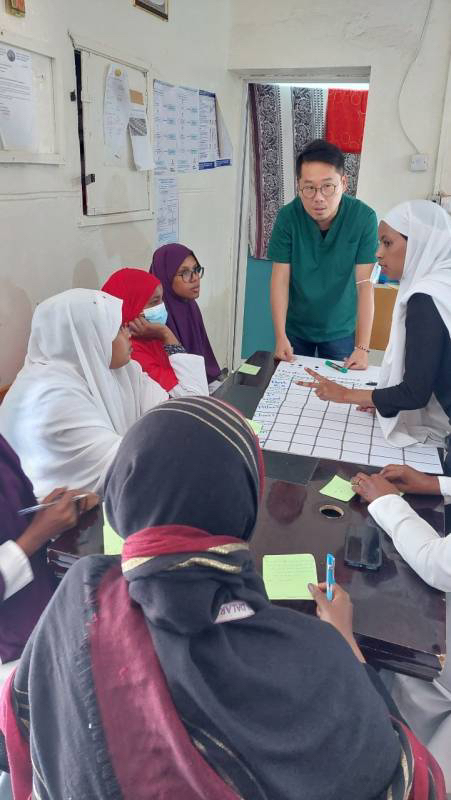
\includegraphics[width=0.30\textwidth]{6963.jpg}
        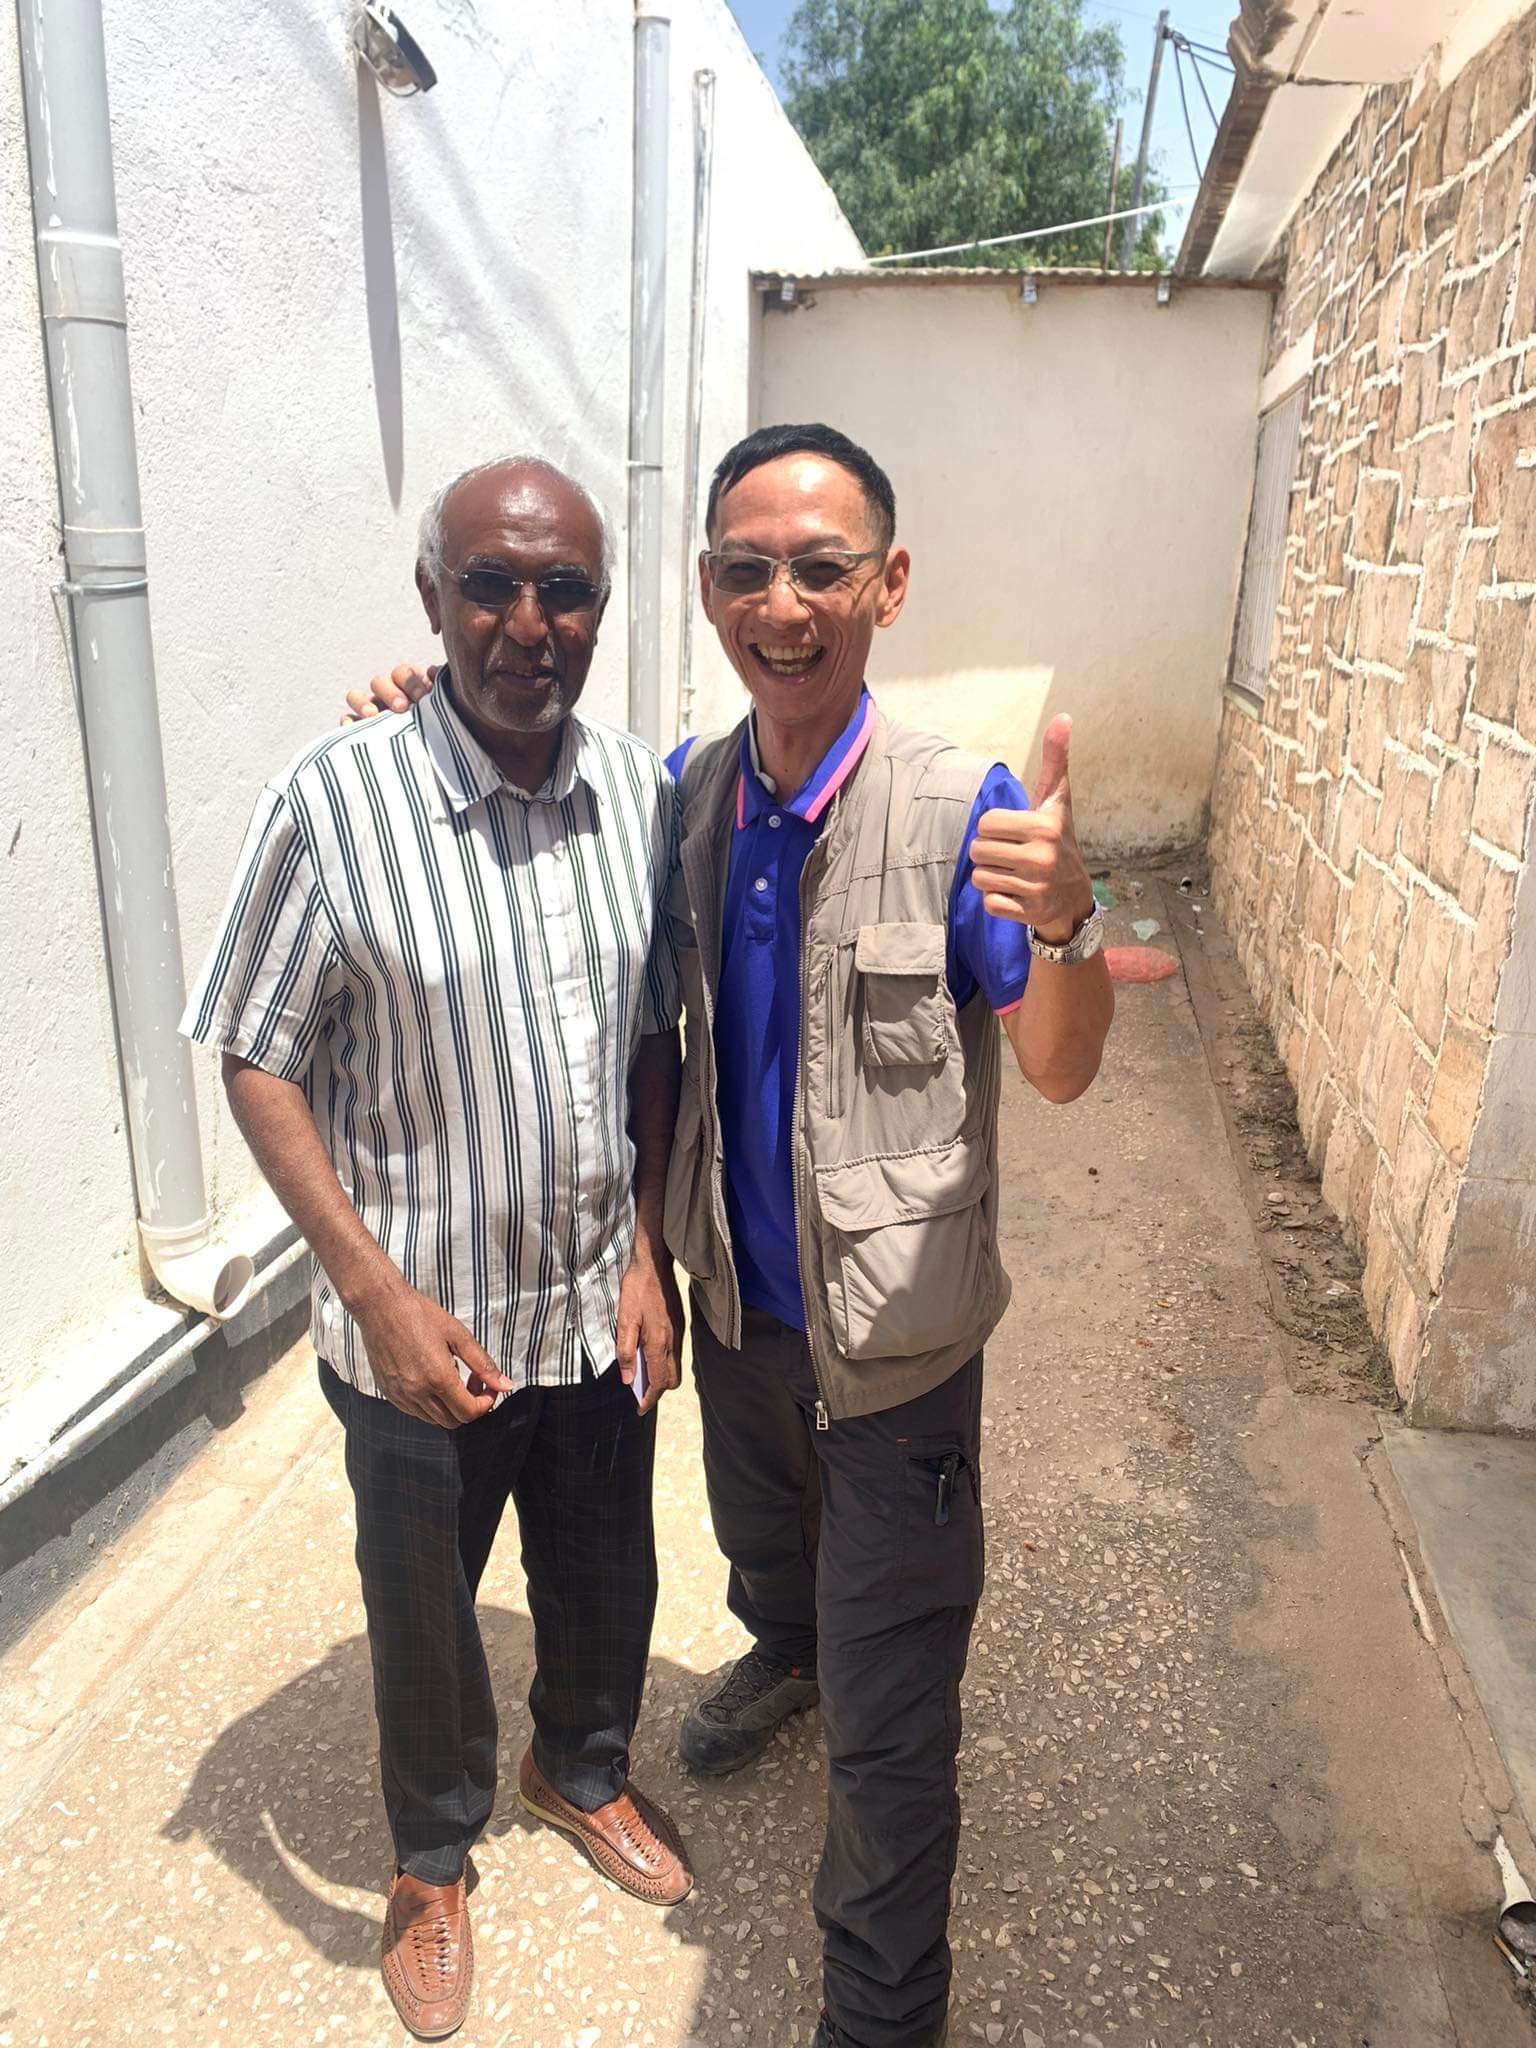
\includegraphics[width=0.30\textwidth]{IMG_5040.jpeg}
    \end{center}
\end{frame}



\begin{frame}{Capacity building: trauma kits supplies}
    \begin{center}
        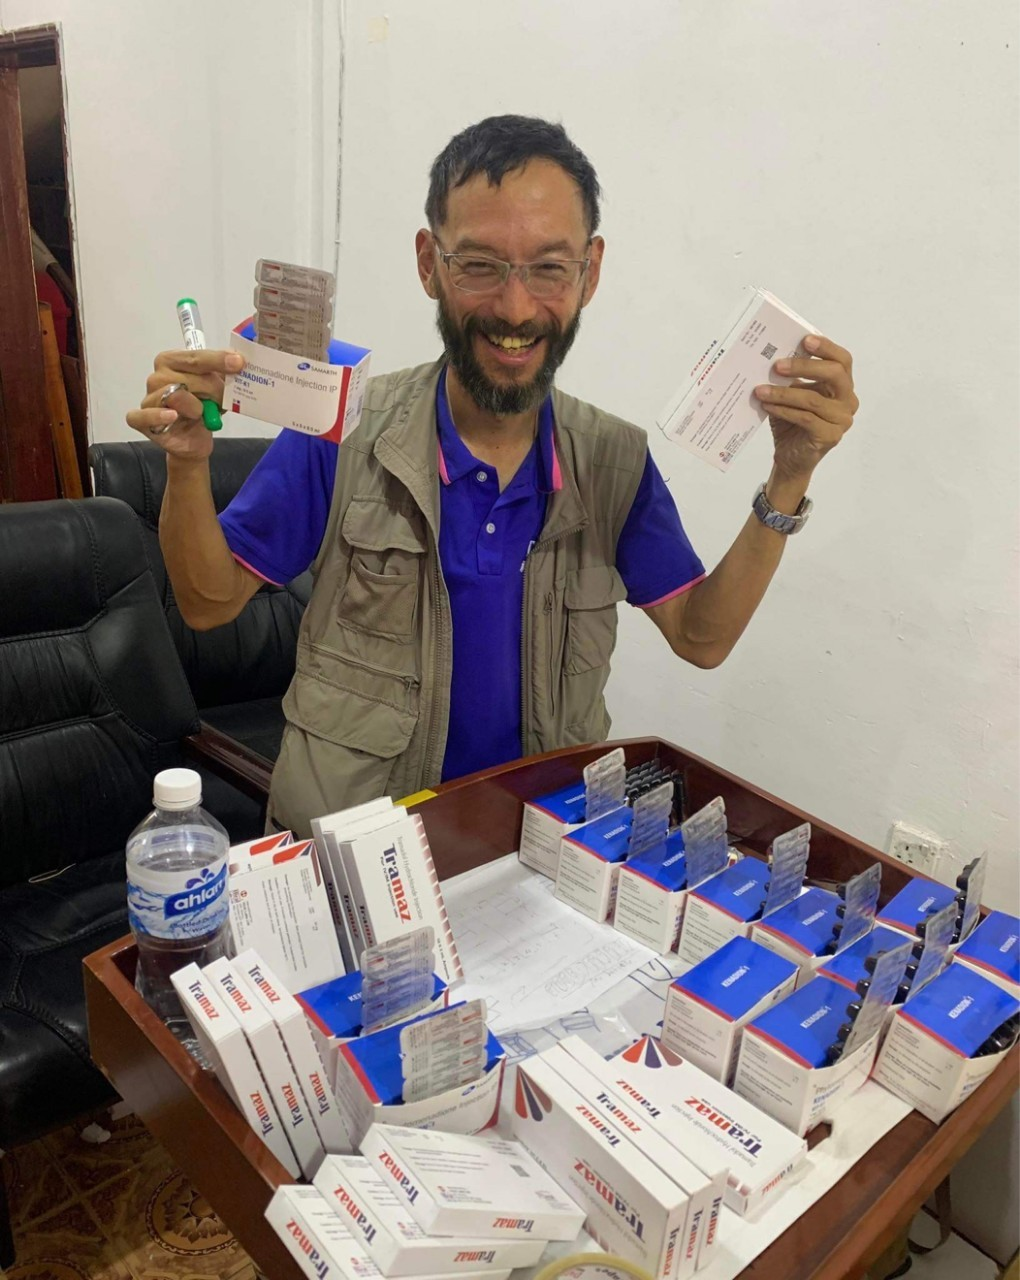
\includegraphics[width=0.33\textwidth]{4875890938550512937.32a296a9eebb4034c36c698f4a25d9d0.23050612.JPG}
        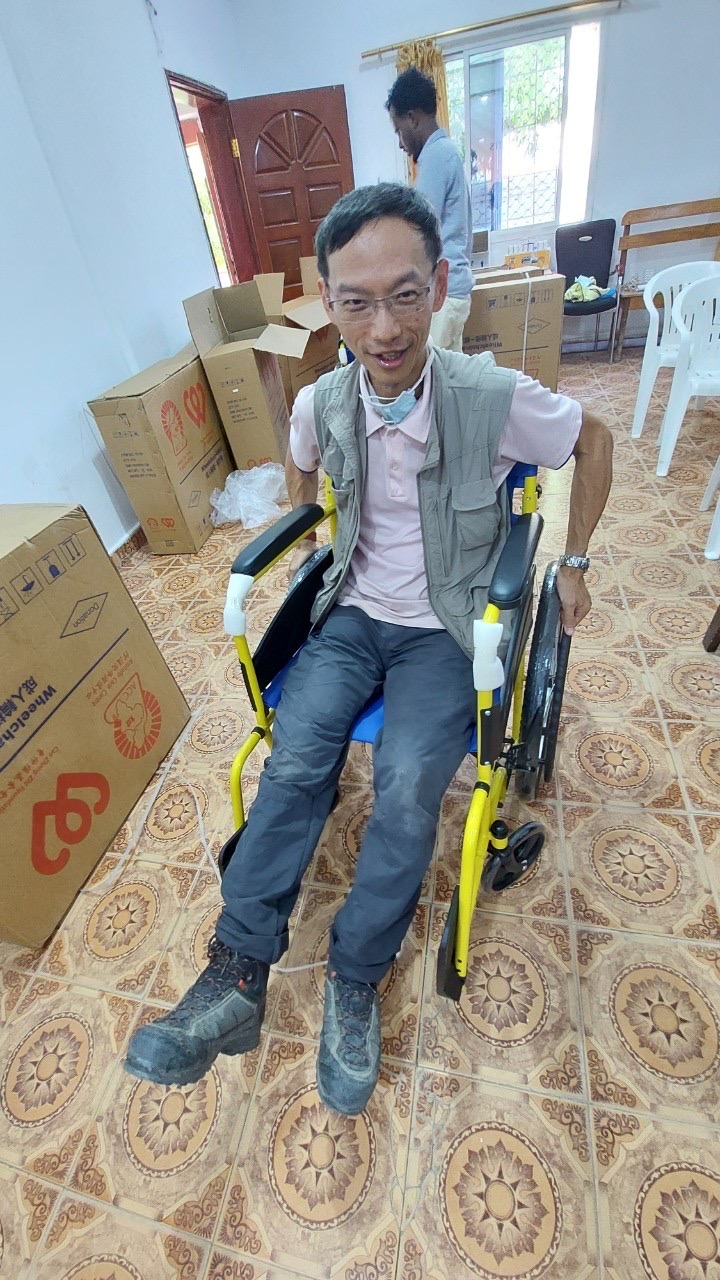
\includegraphics[width=0.30\textwidth]{IMG-2655.JPG}
        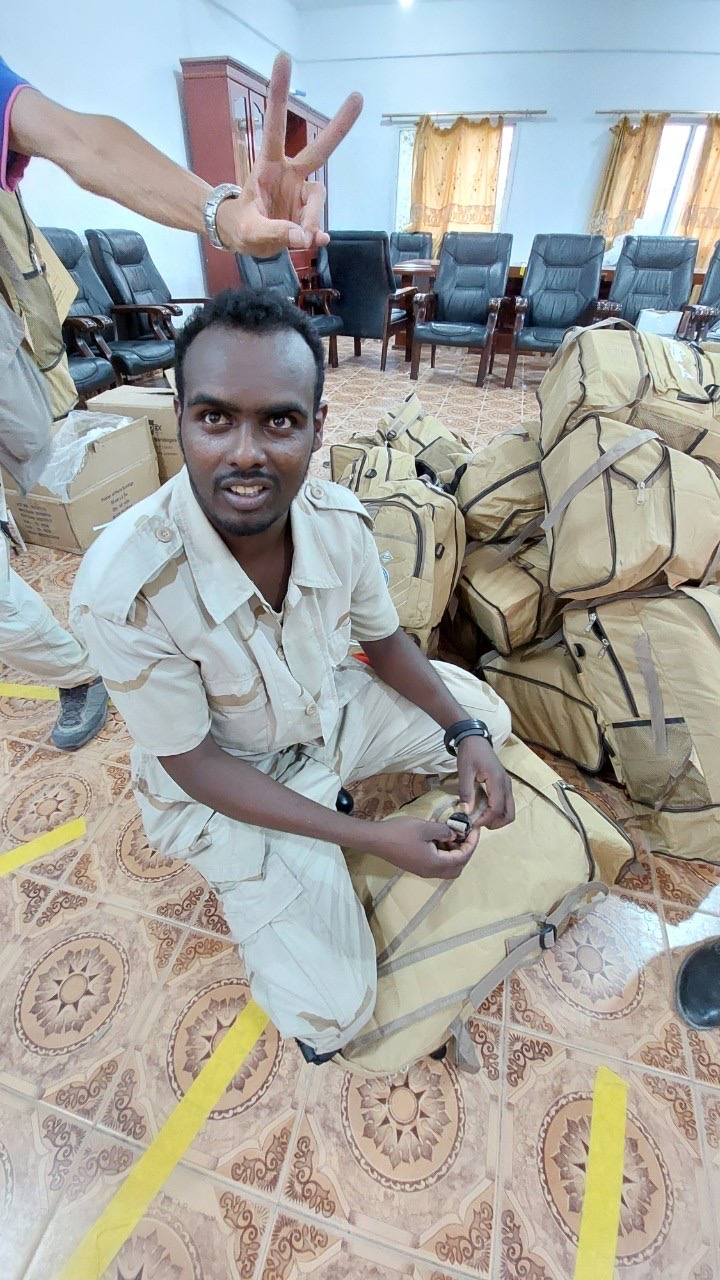
\includegraphics[width=0.30\textwidth]{IMG-2313.JPG}
%        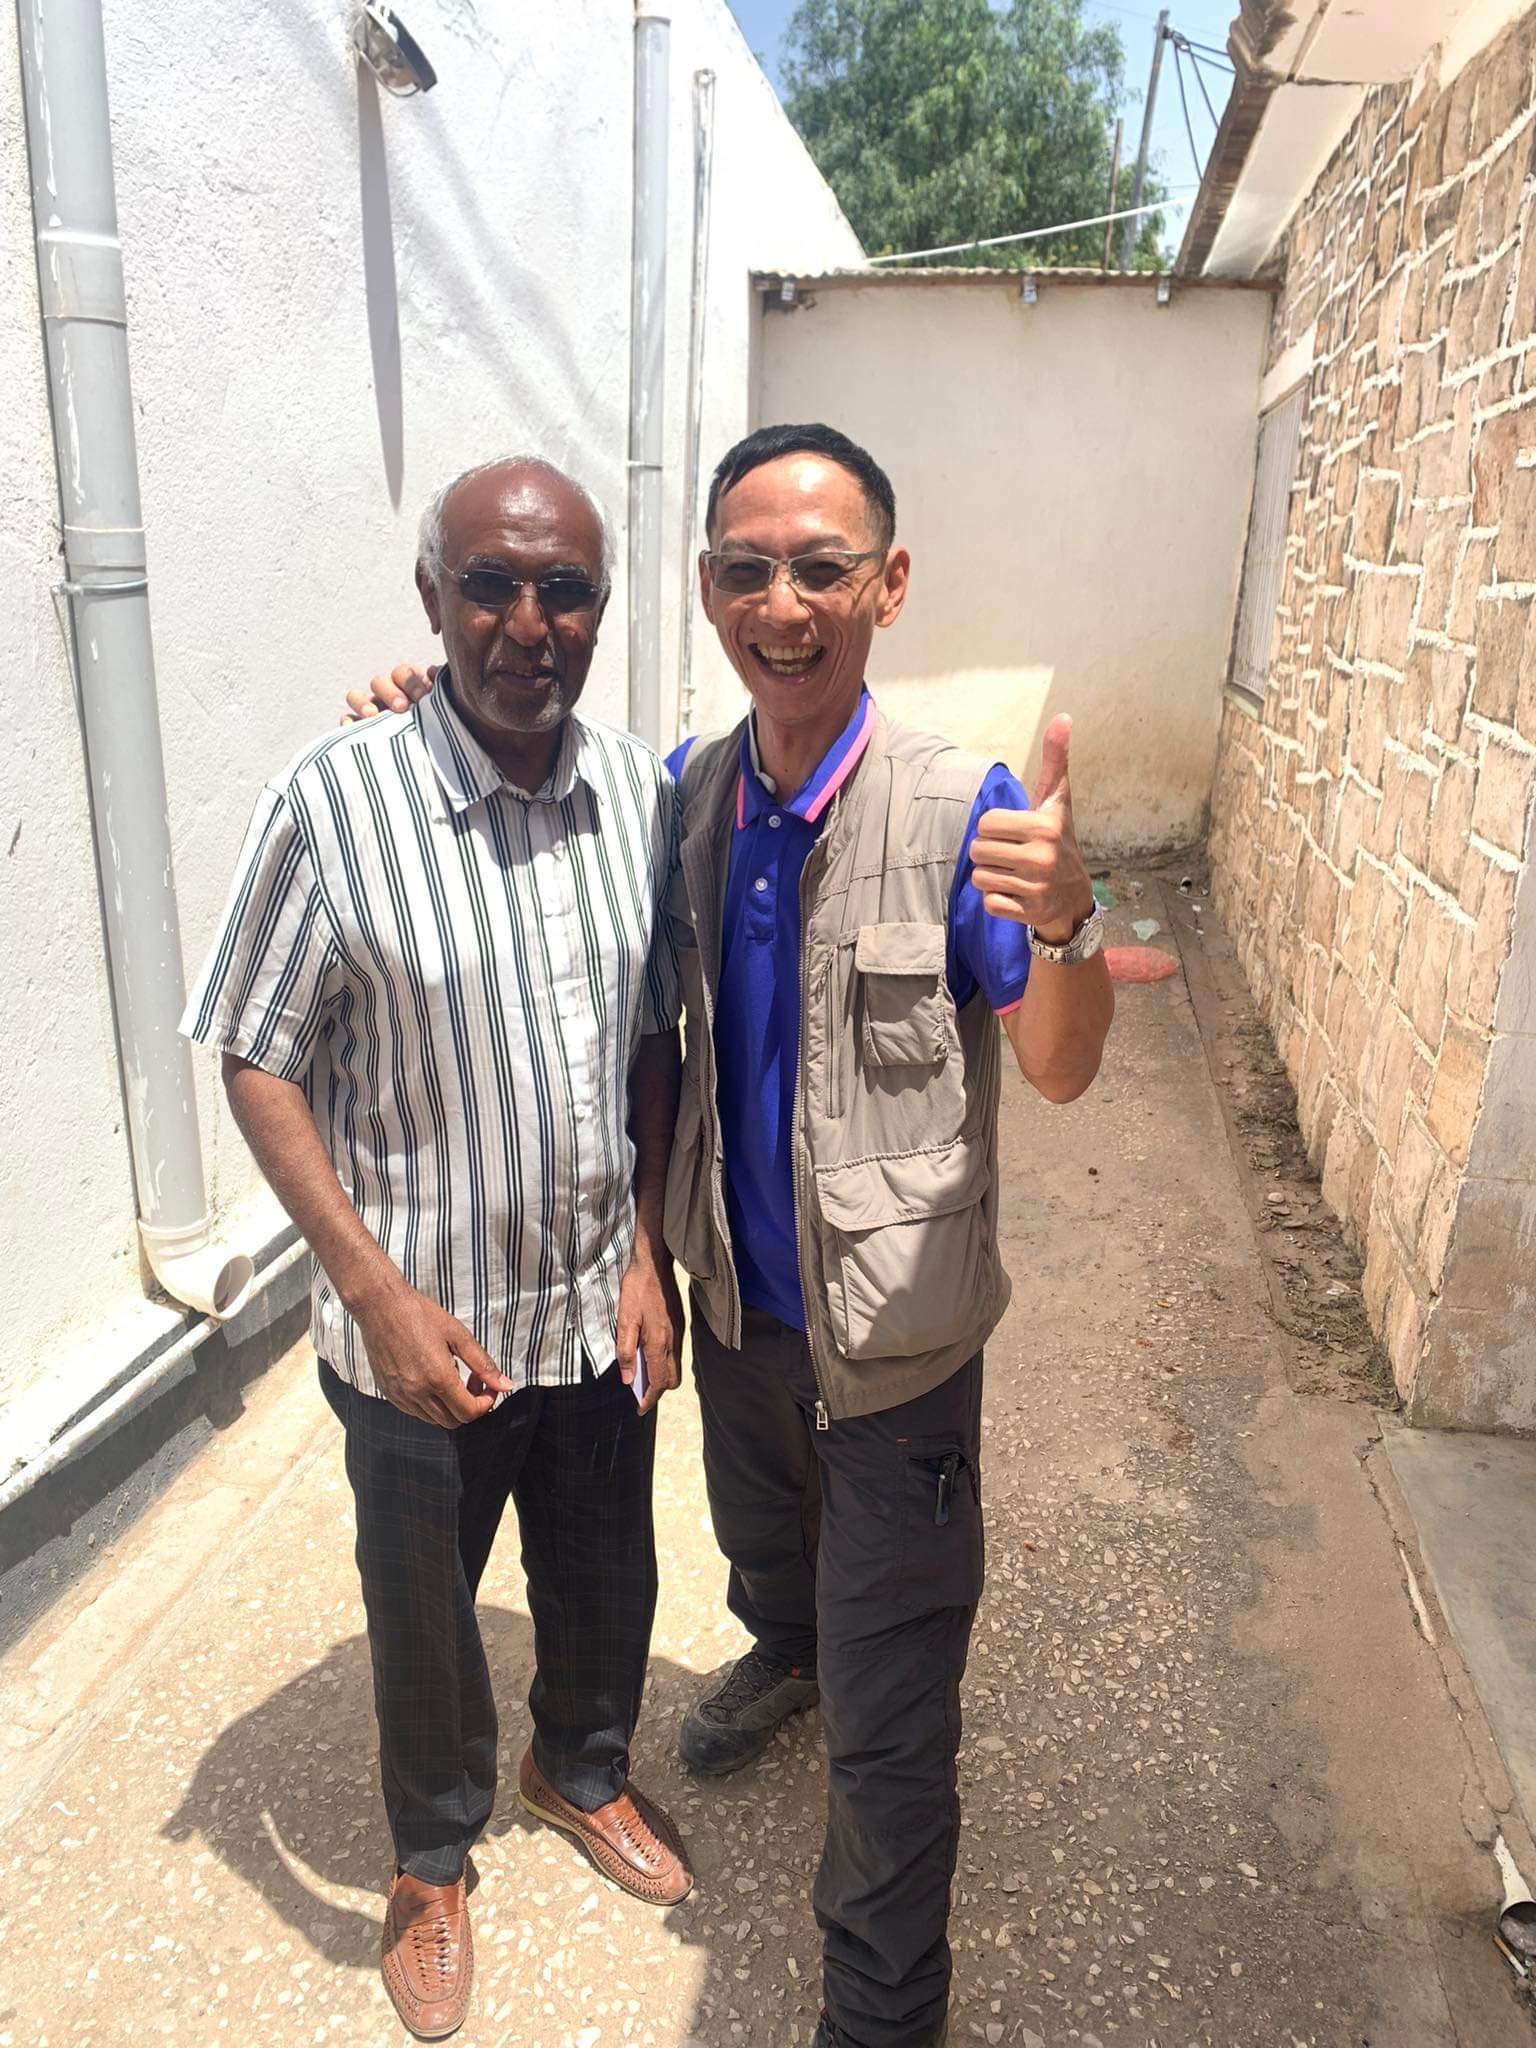
\includegraphics[width=0.24\textwidth]{IMG_5040.jpeg}    
    \end{center}
\end{frame}

\begin{frame}{Capacity building: trauma kits supplies}
    \begin{center}
        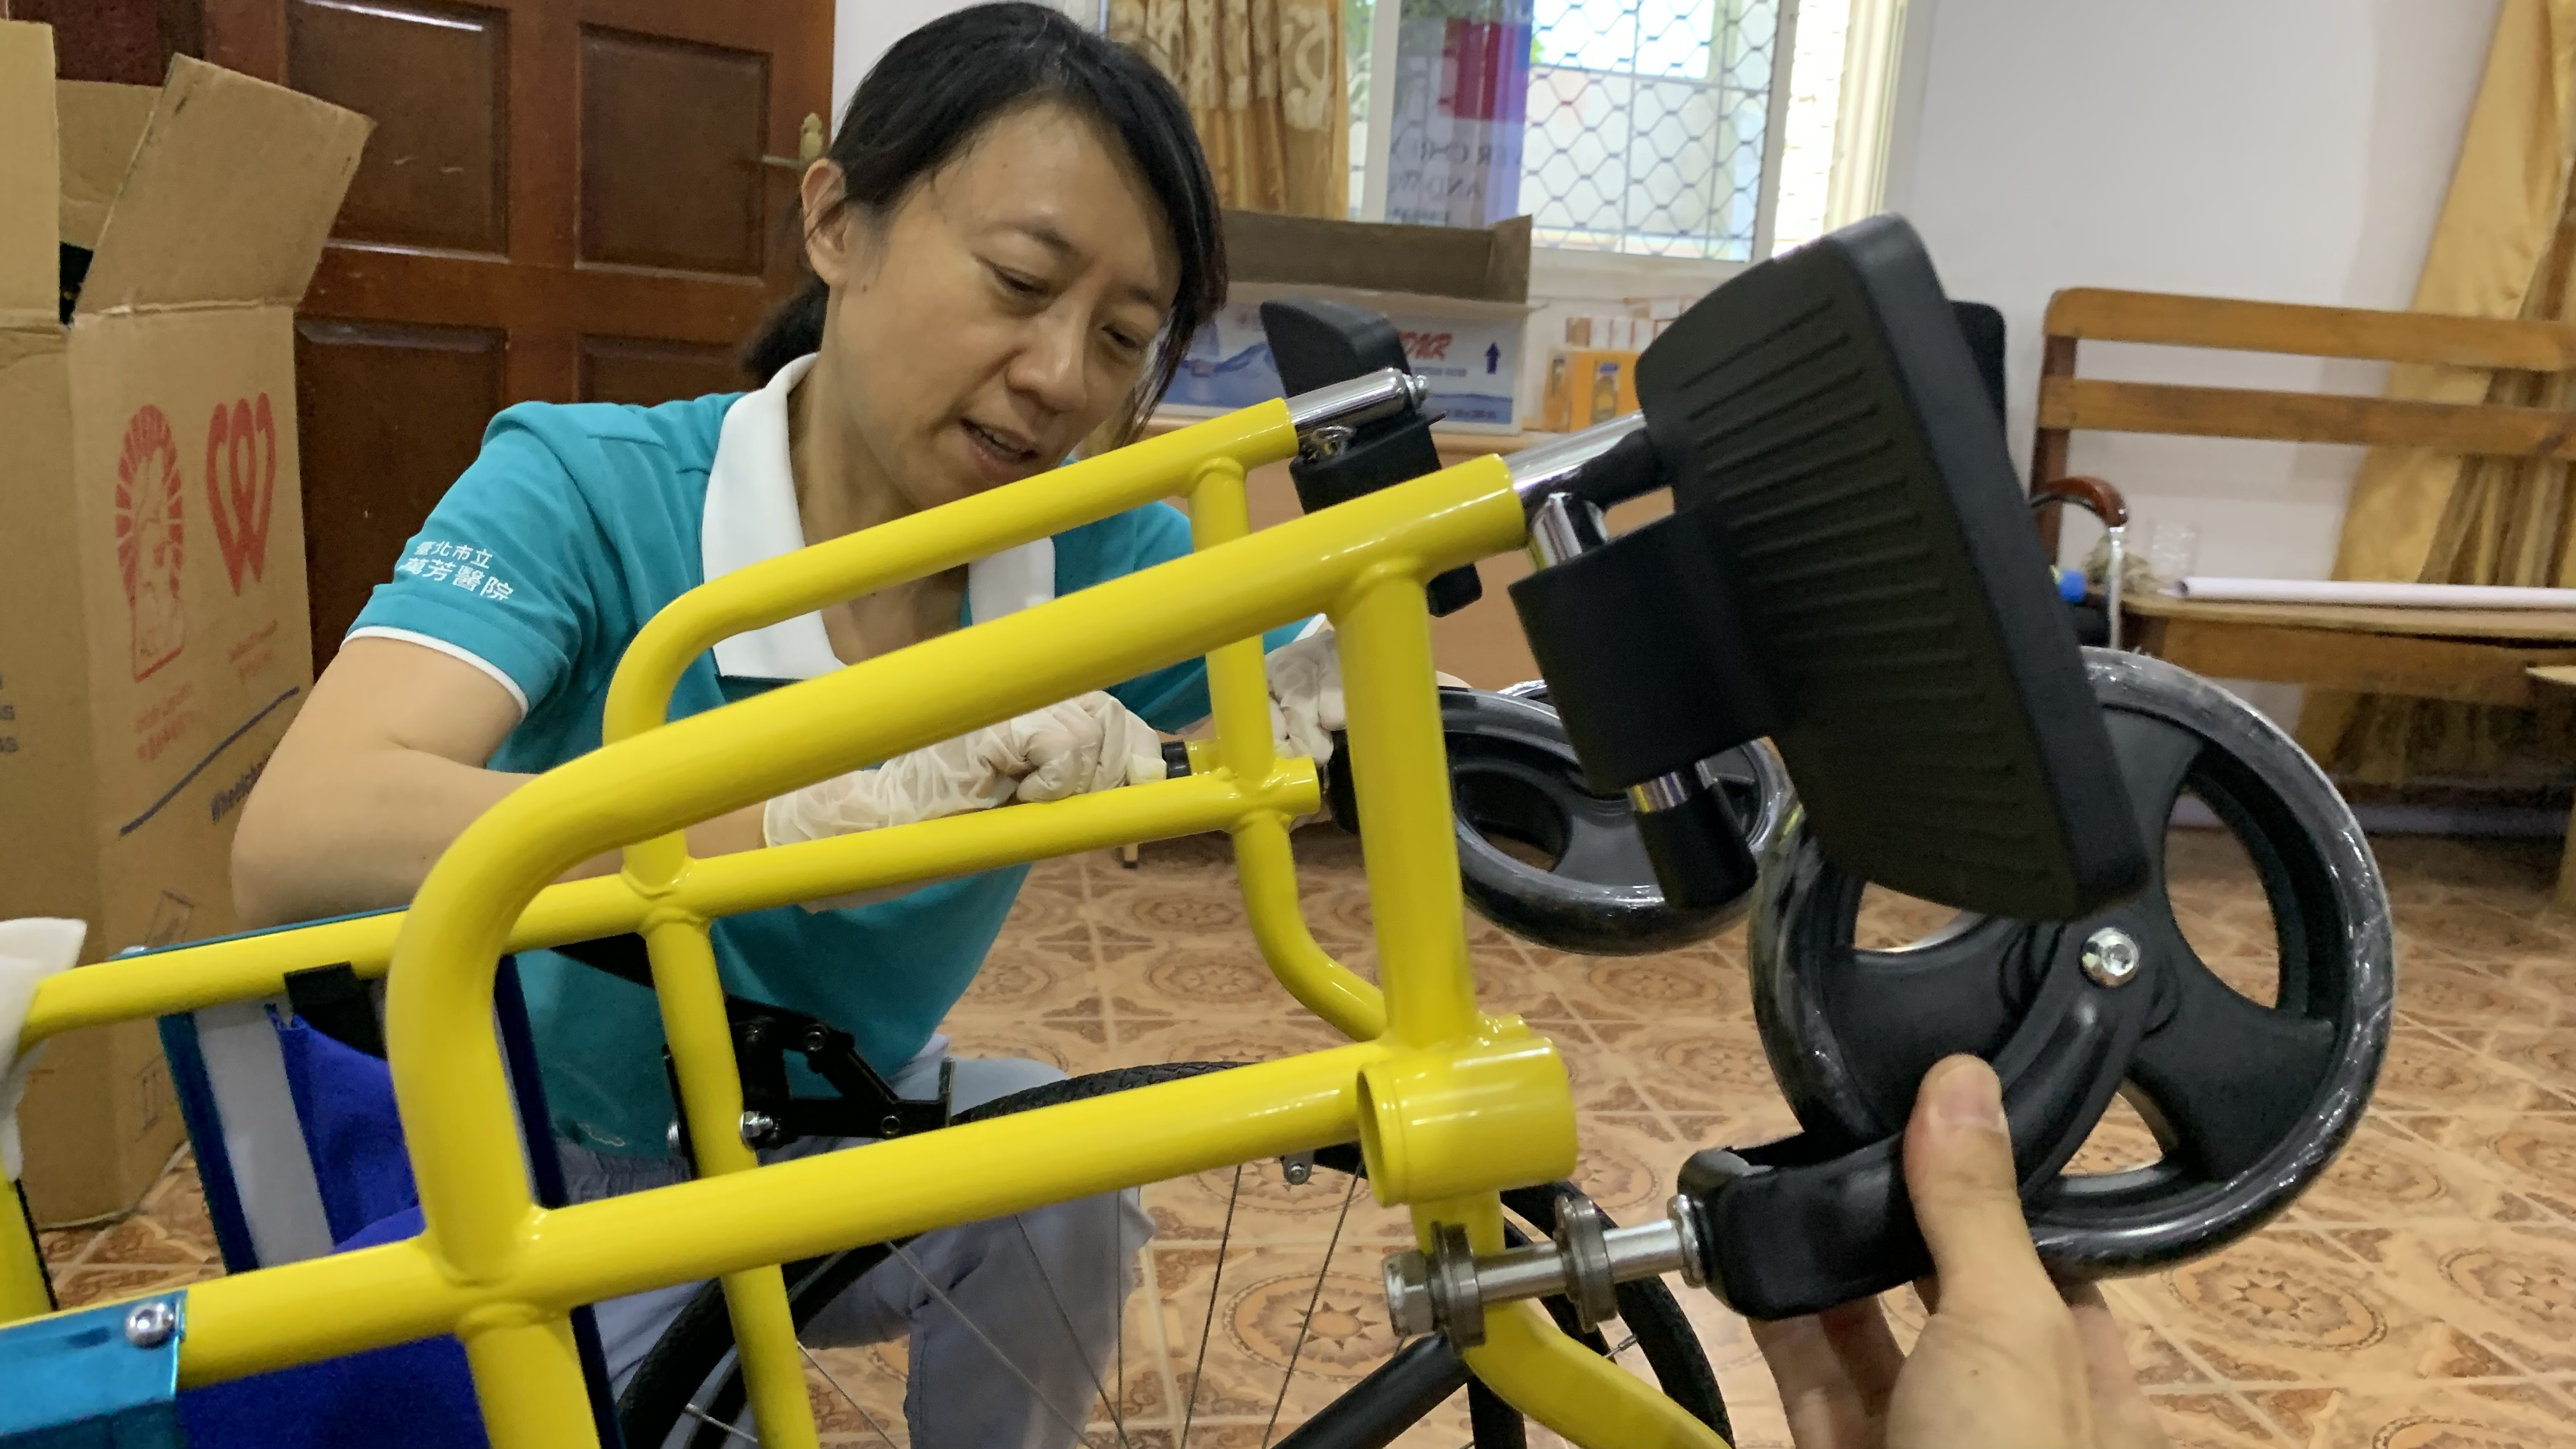
\includegraphics[width=0.4\textwidth]{IMG-2641.jpg}
        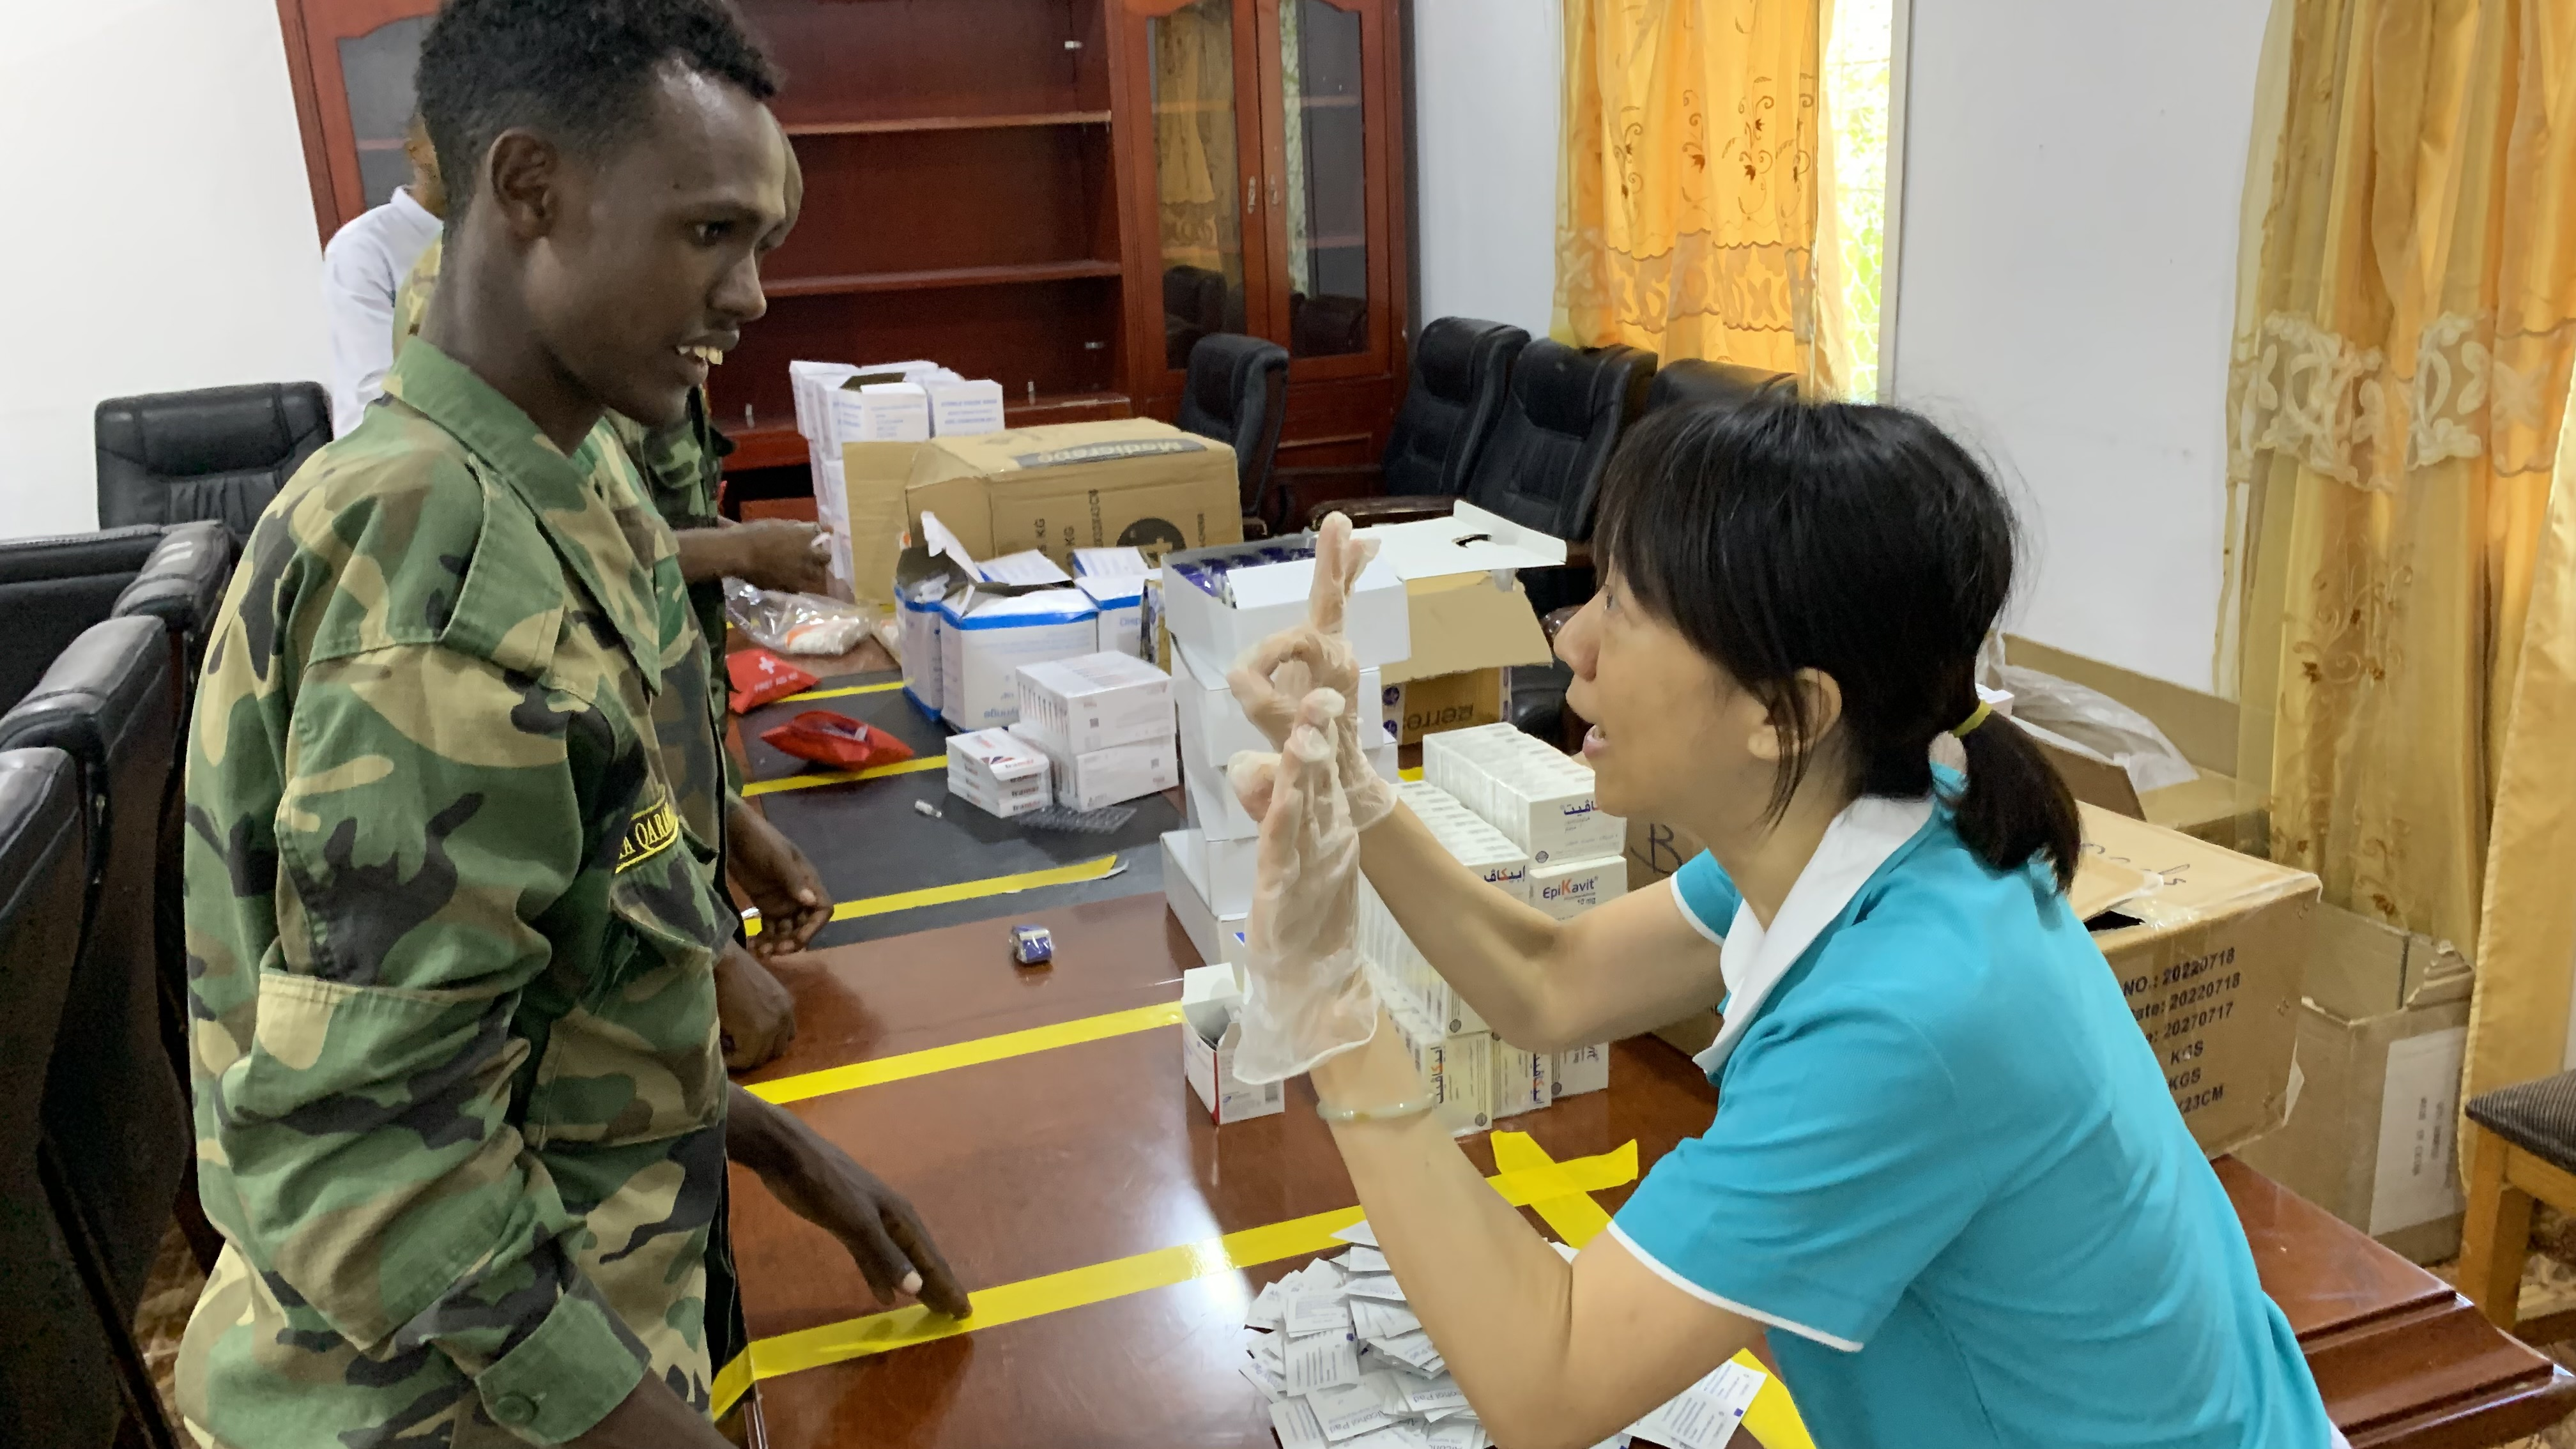
\includegraphics[width=0.4\textwidth]{IMG-2230.jpg} \\
        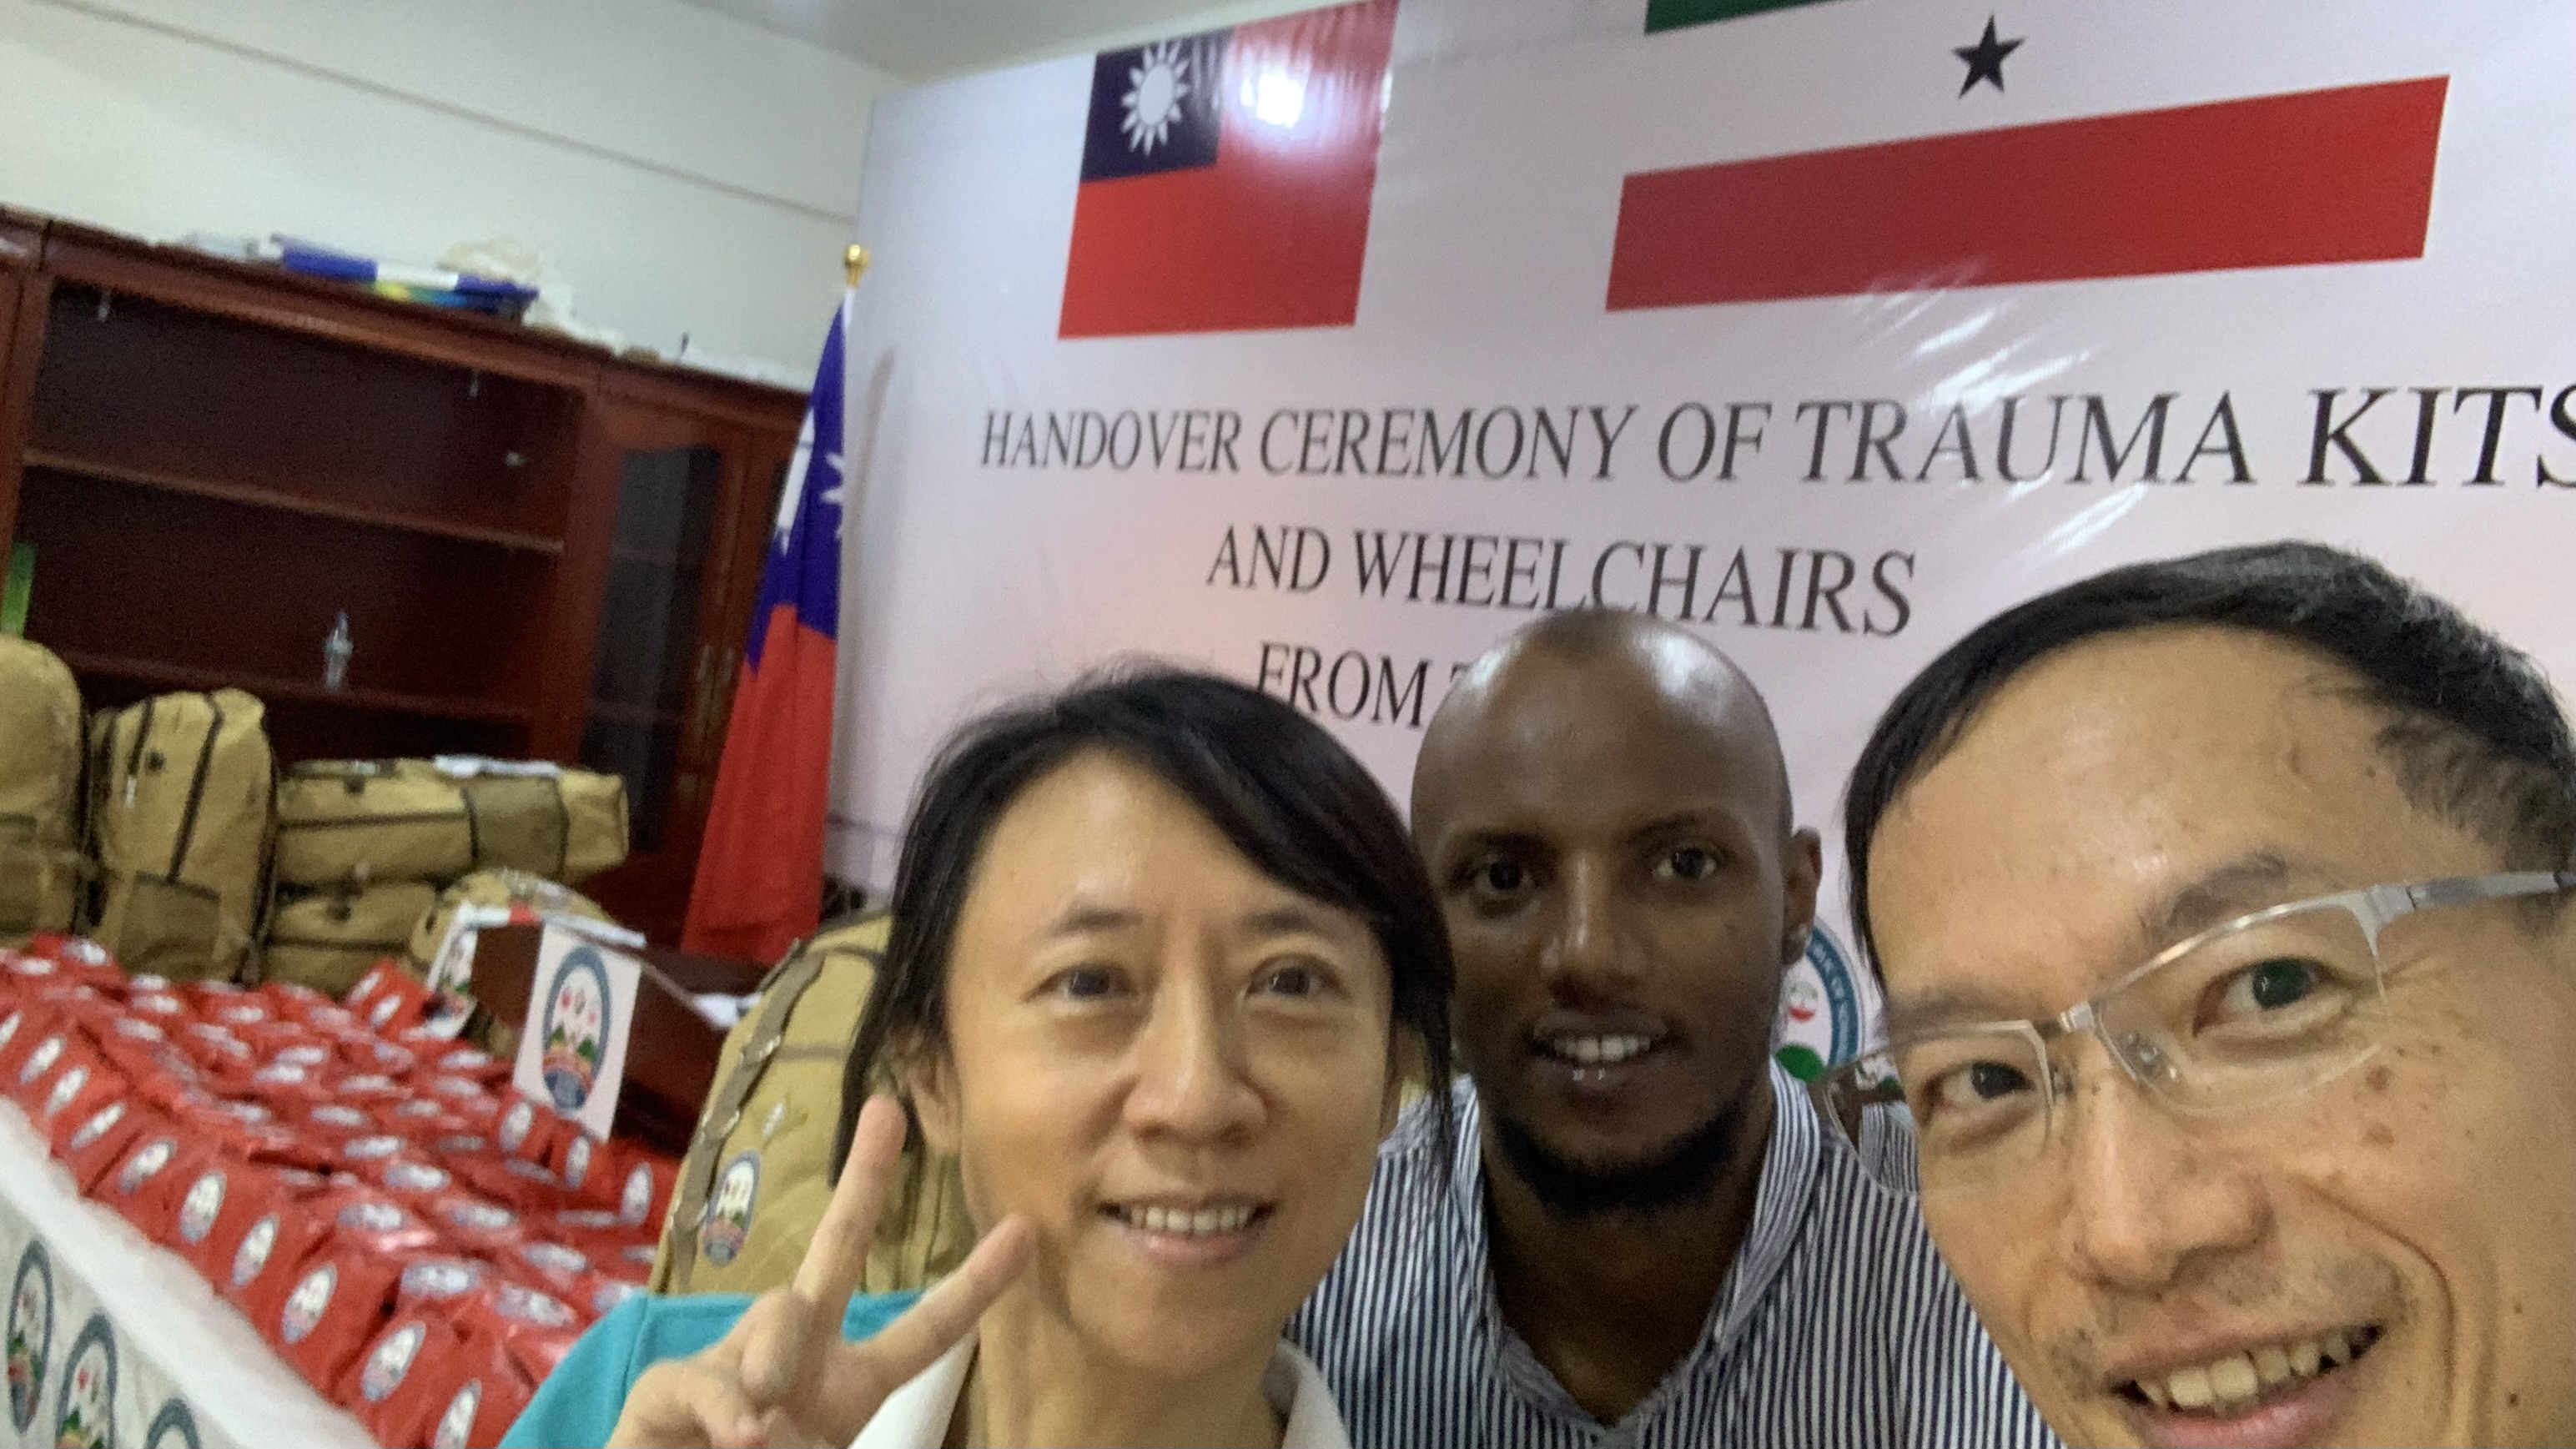
\includegraphics[width=0.4\textwidth]{IMG-2611.jpg}
        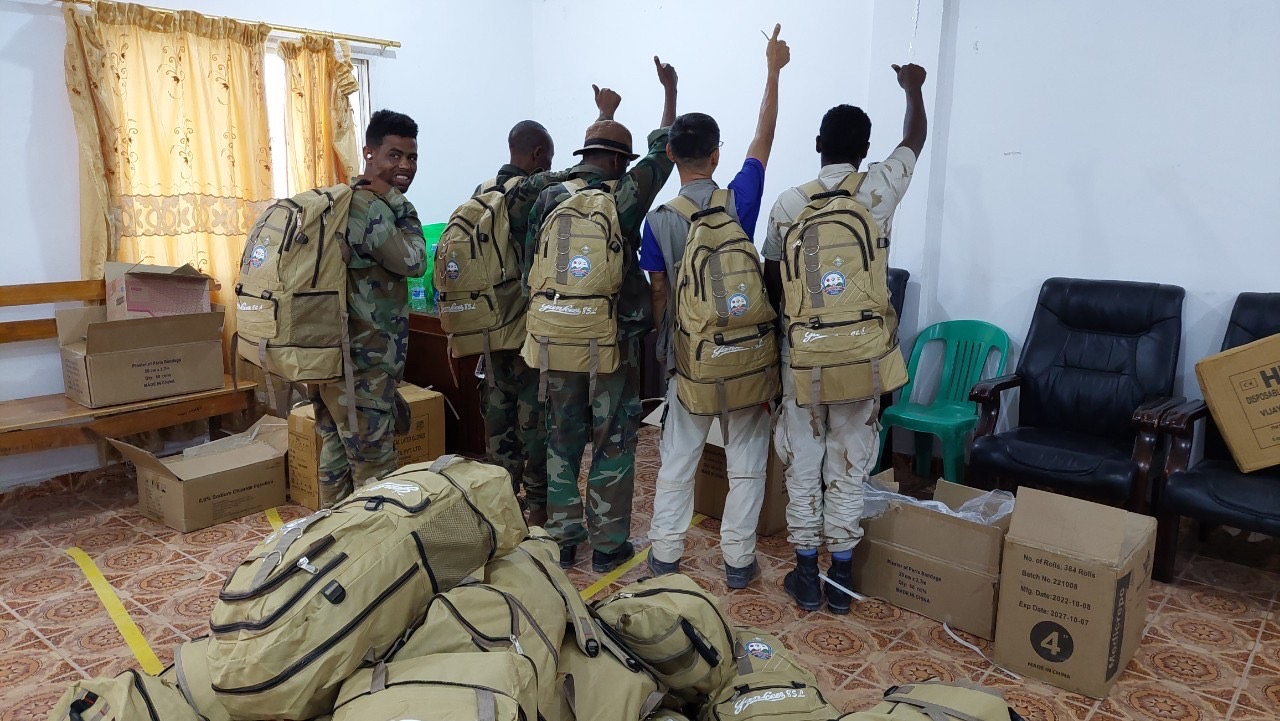
\includegraphics[width=0.4\textwidth]{IMG-2318.JPG}    
    \end{center}
\end{frame}

%%
\begin{frame}{Capacity building: trauma kits supplies}
    \begin{center}
        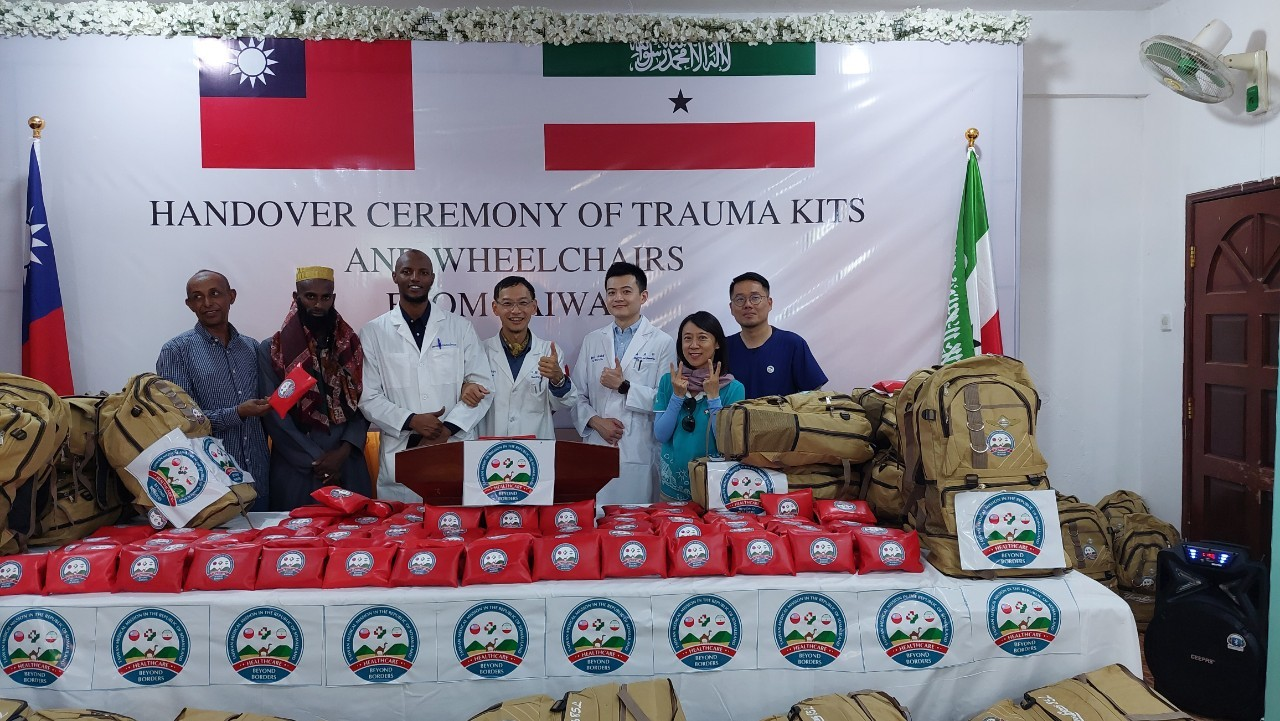
\includegraphics[width=0.8\textwidth]{4879921870343011711.12ba1a84484c21cdb54161b56f33e999.23050712.JPG}
    \end{center}
\end{frame}

\begin{frame}{Capacity building: others}
    \begin{center}
        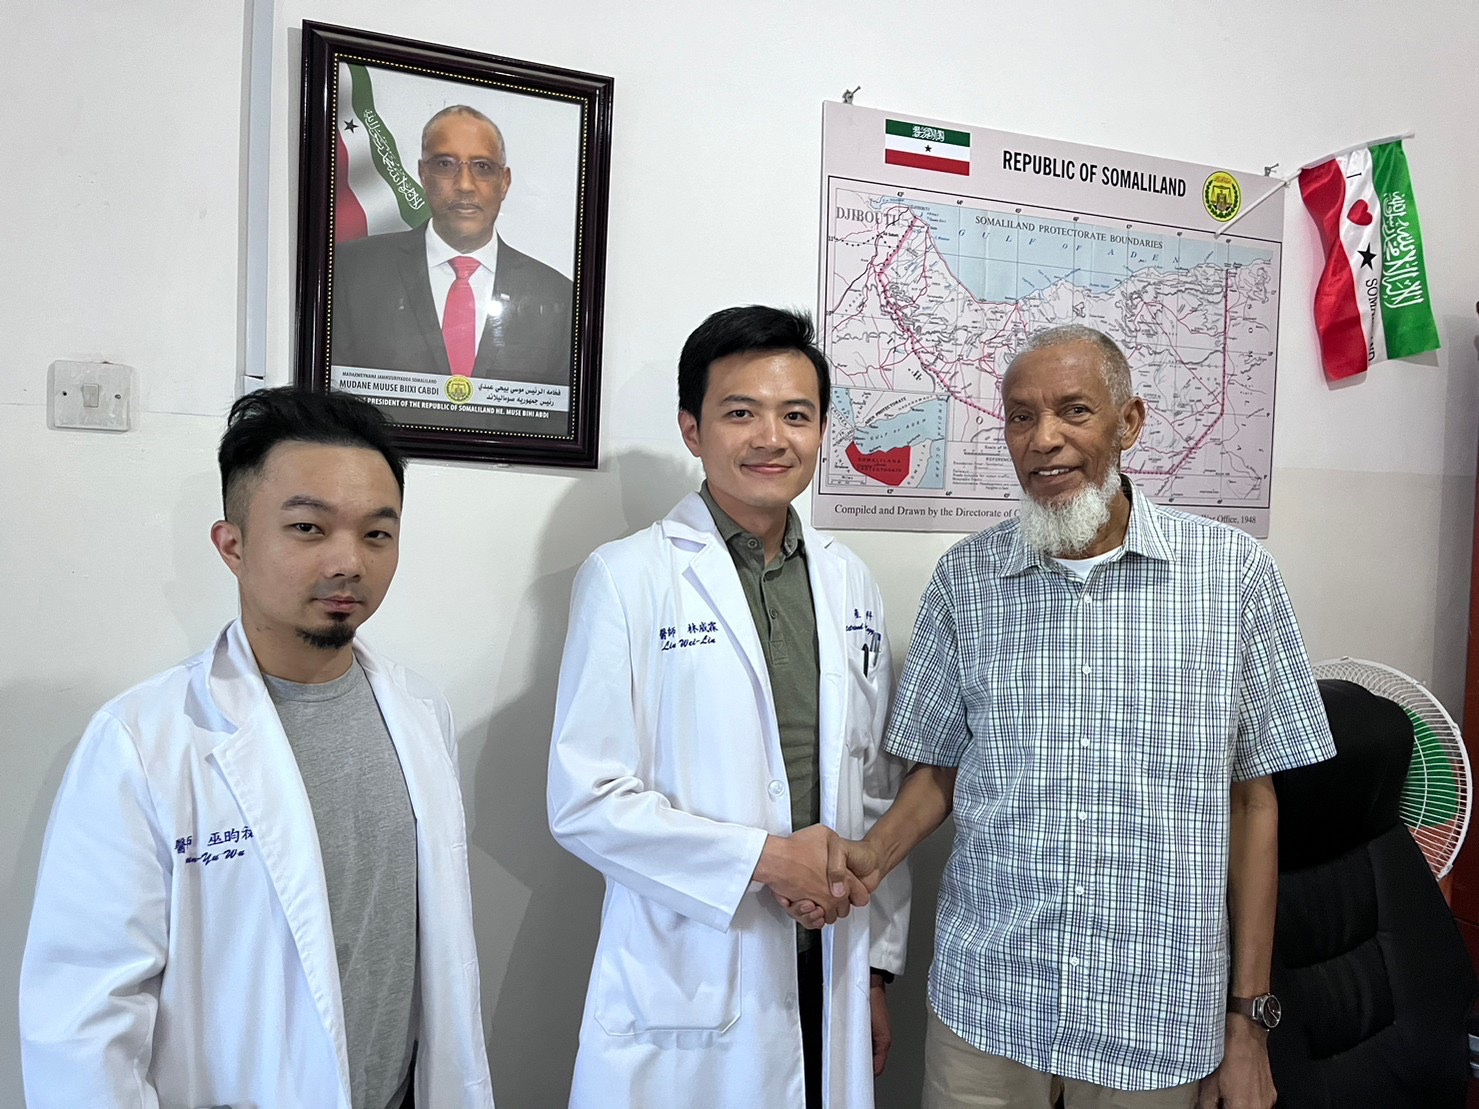
\includegraphics[width=0.24\textwidth]{IMG-5107.JPG}
        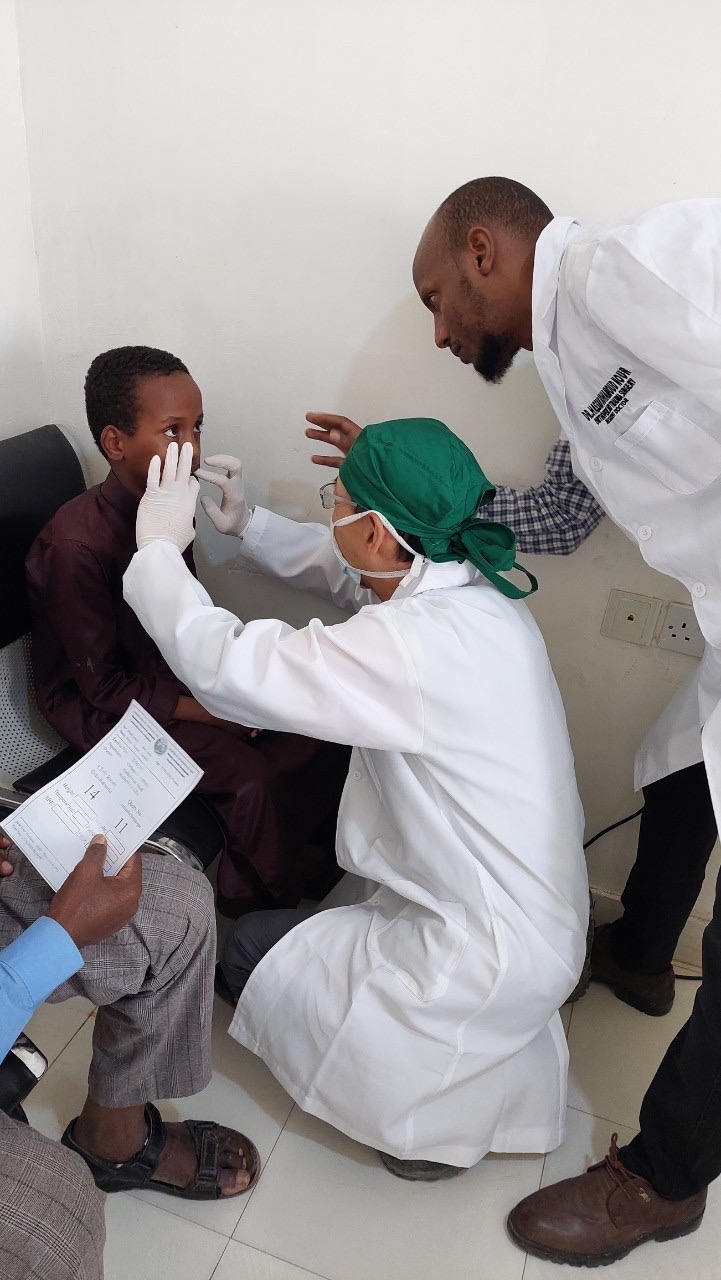
\includegraphics[width=0.24\textwidth]{IMG-4703.JPG}
        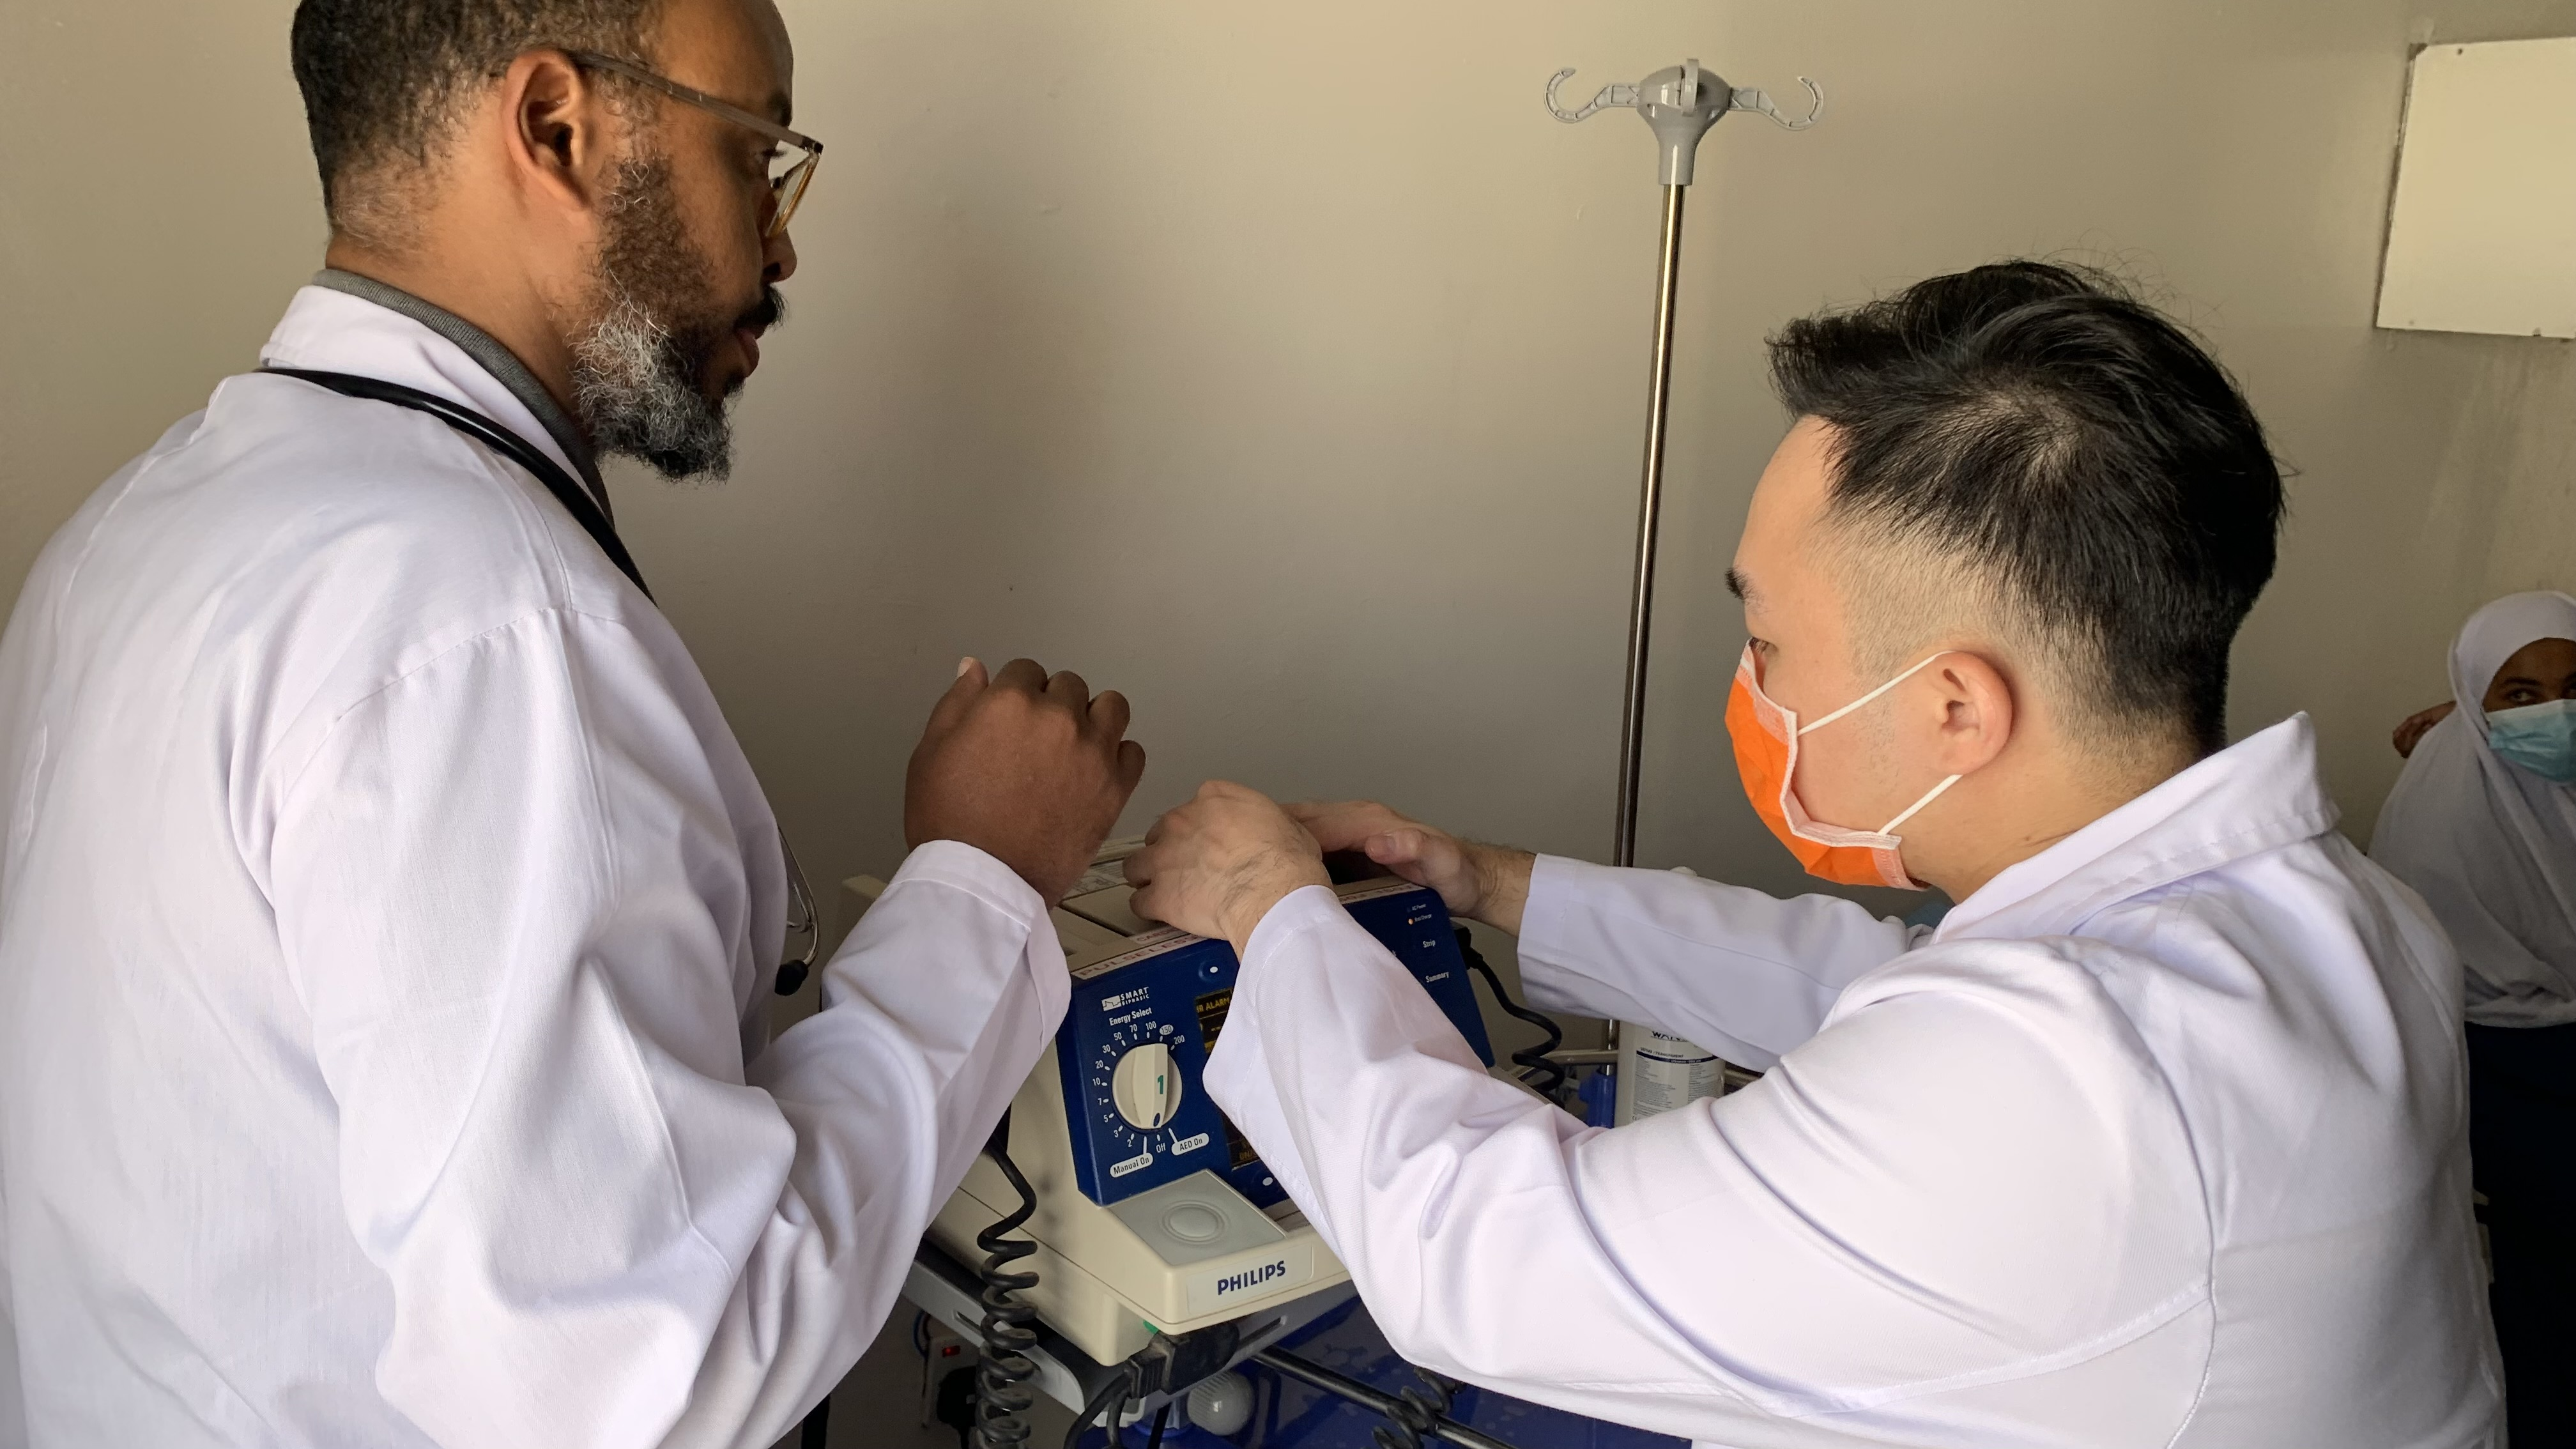
\includegraphics[width=0.24\textwidth]{IMG-5062.JPG}
        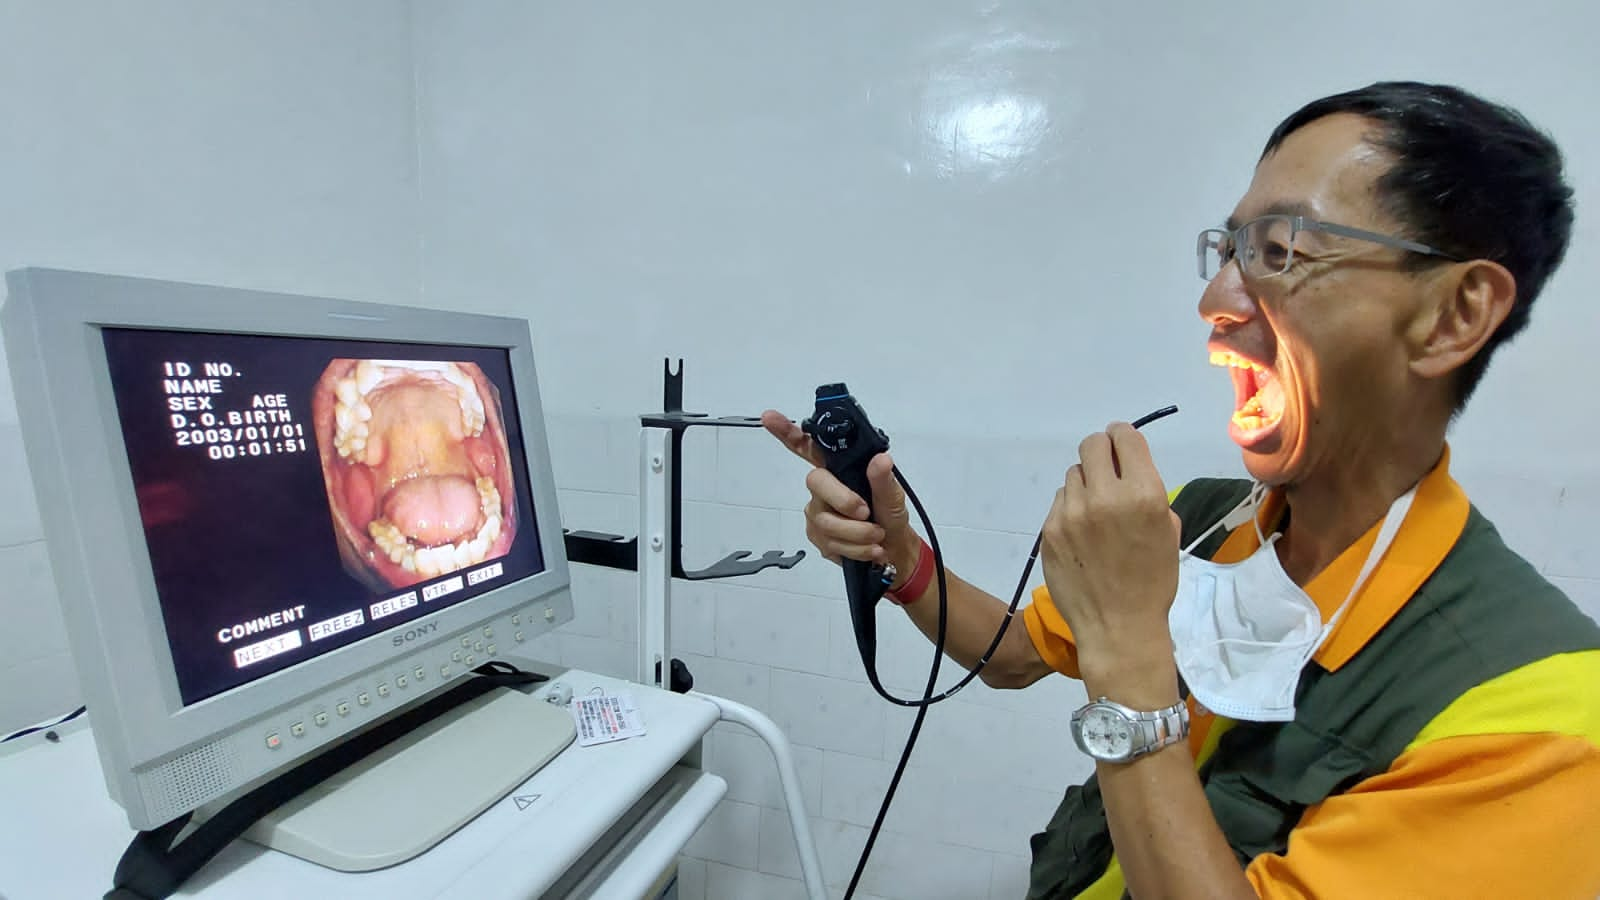
\includegraphics[width=0.24\textwidth]{6a625355-ae53-4e8f-891e-38a933f6c29b.JPG}    
    \end{center}
\end{frame}
%%    
\begin{frame}
\frametitle{TMM's Projects - third pillar}
% Add content here
\begin{outline}    
    \1 public health, we are launching
        \2 World Blood Donor Day campaign (2023/06/14)
        \2 Pap smear screen for elimination of cervical cancer (July 2023)
        \2 Good oral hygiene and oral cancer screening (March 2024)
        \2 HBV/HCV screenings, vaccinations, and treatment (2023/07/28)
        \2 Osteoprosis screening for women who get vitamin D deficience (Oct 2023)
        \2 Parasite screening program for schoolchildren (2024)
\end{outline}

\begin{center}
\includesvg[width=0.14\textwidth]{Blood_logo.svg}
\includesvg[width=0.14\textwidth]{anti_CervicalCancer_logo.svg}
\includesvg[width=0.22\textwidth]{World_OralHealth_Day_logo.svg}
\includesvg[width=0.14\textwidth]{WHD_logo.svg}
\includesvg[width=0.2\textwidth]{parasite_logo.svg}
\end{center}

\end{frame}

\begin{frame}{Public health: Oral health}
    \begin{columns}
        
    \column{0.5\textwidth}
        \begin{center}
        \includesvg[width=0.7\textwidth]{World_OralHealth_Day_logo.svg}
            
        \end{center}
    \column{0.5\textwidth}
        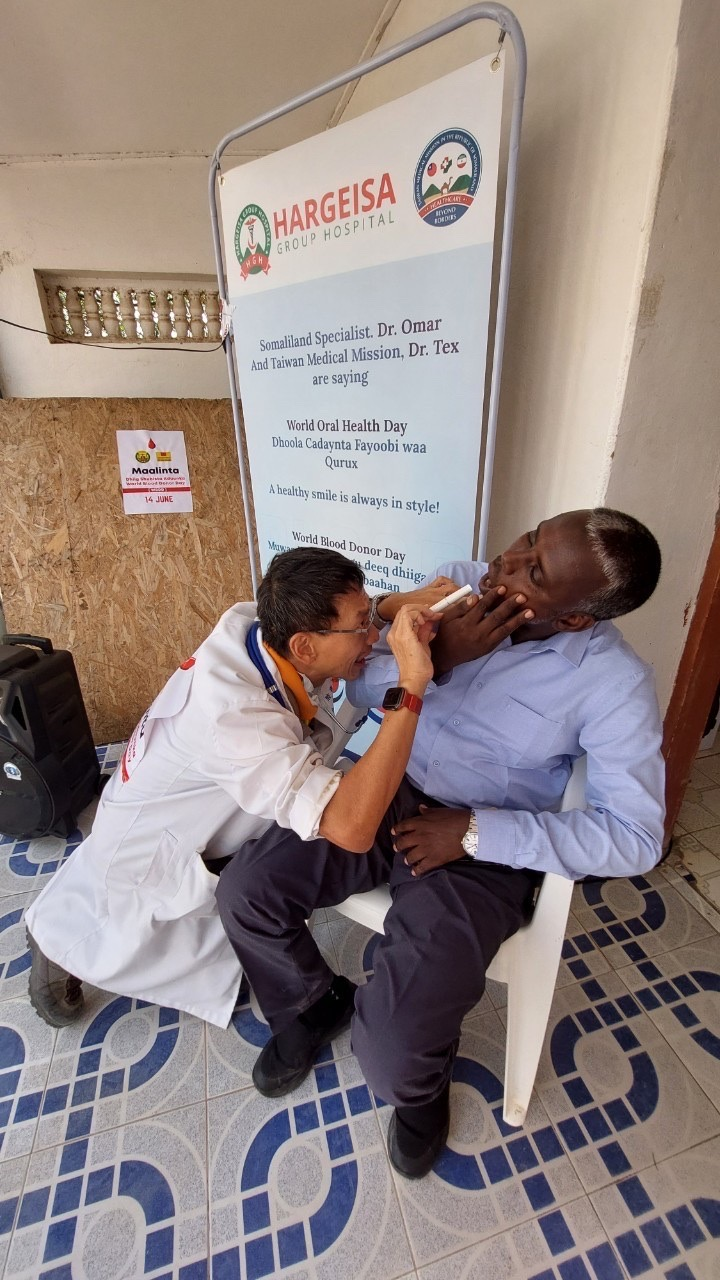
\includegraphics[width=0.7\textwidth]{IMG-4368.JPG}
%        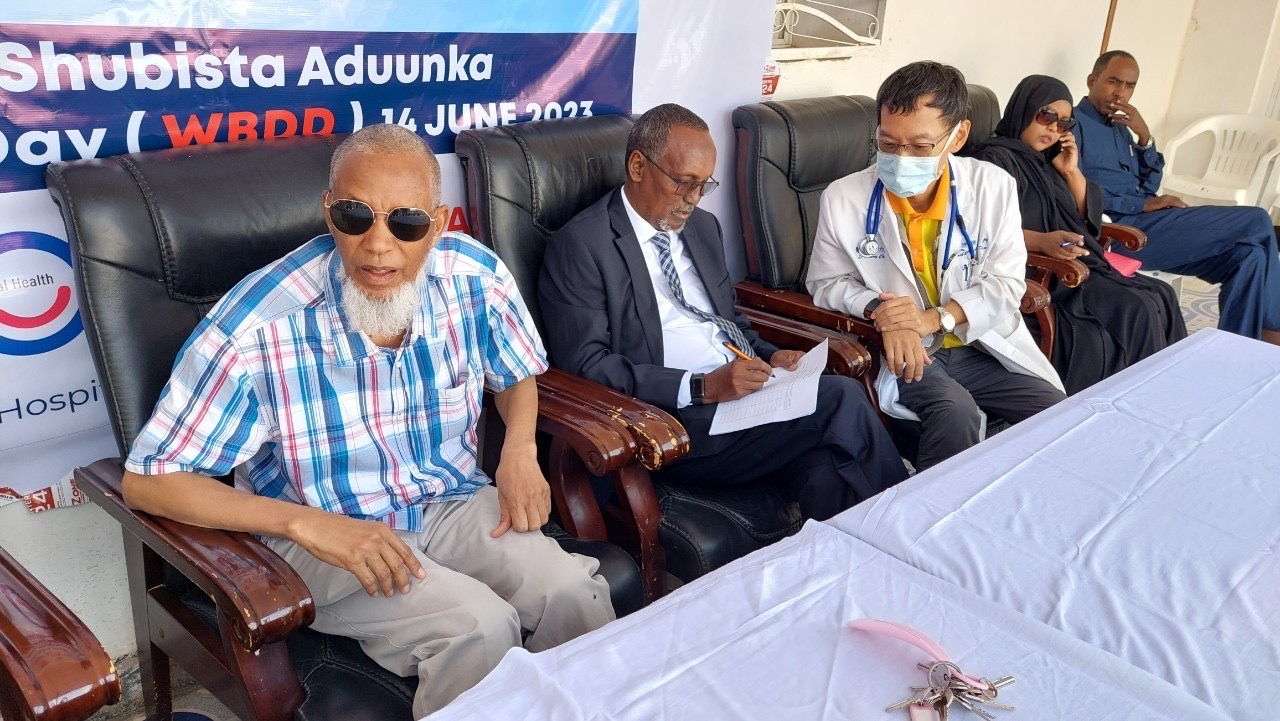
\includegraphics[width=0.45\textwidth]{IMG-4378.JPG}
    \end{columns}
\end{frame}




% Dr Askar
\begin{frame}{Public health: World Blood Donor Day}
    \begin{center}
        \includesvg[width=0.2\textwidth]{Blood_logo.svg}
%        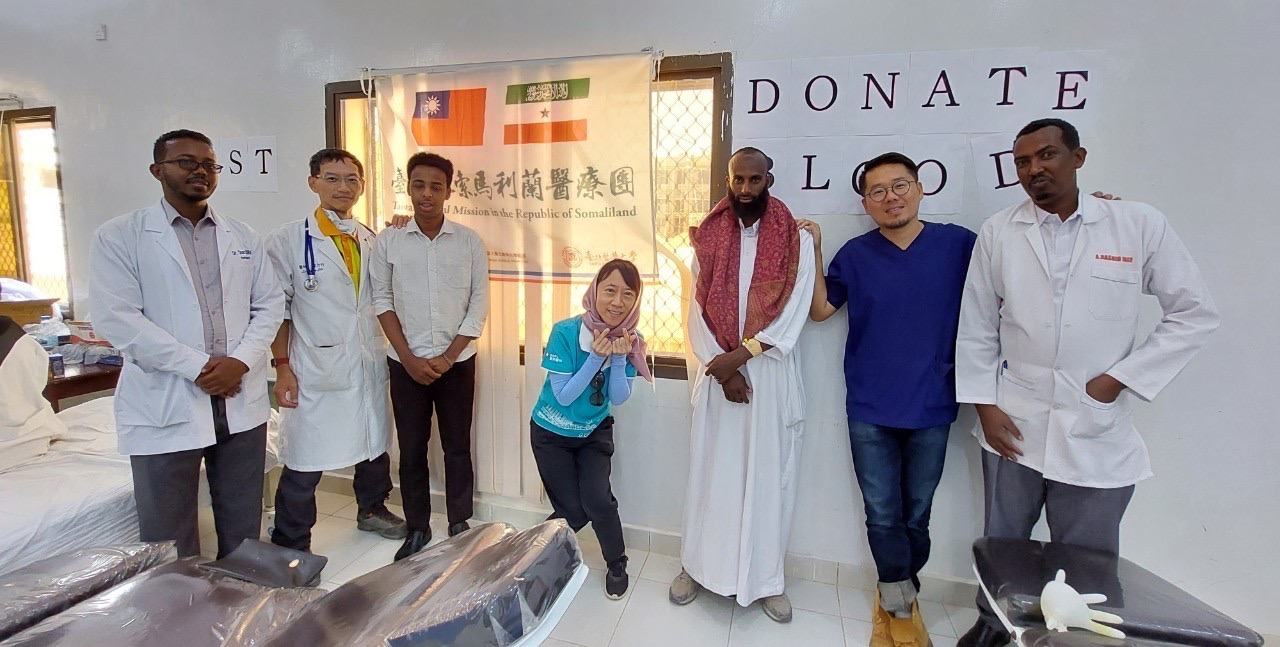
\includegraphics[width=0.35\textwidth]{IMG-4441.JPG}
        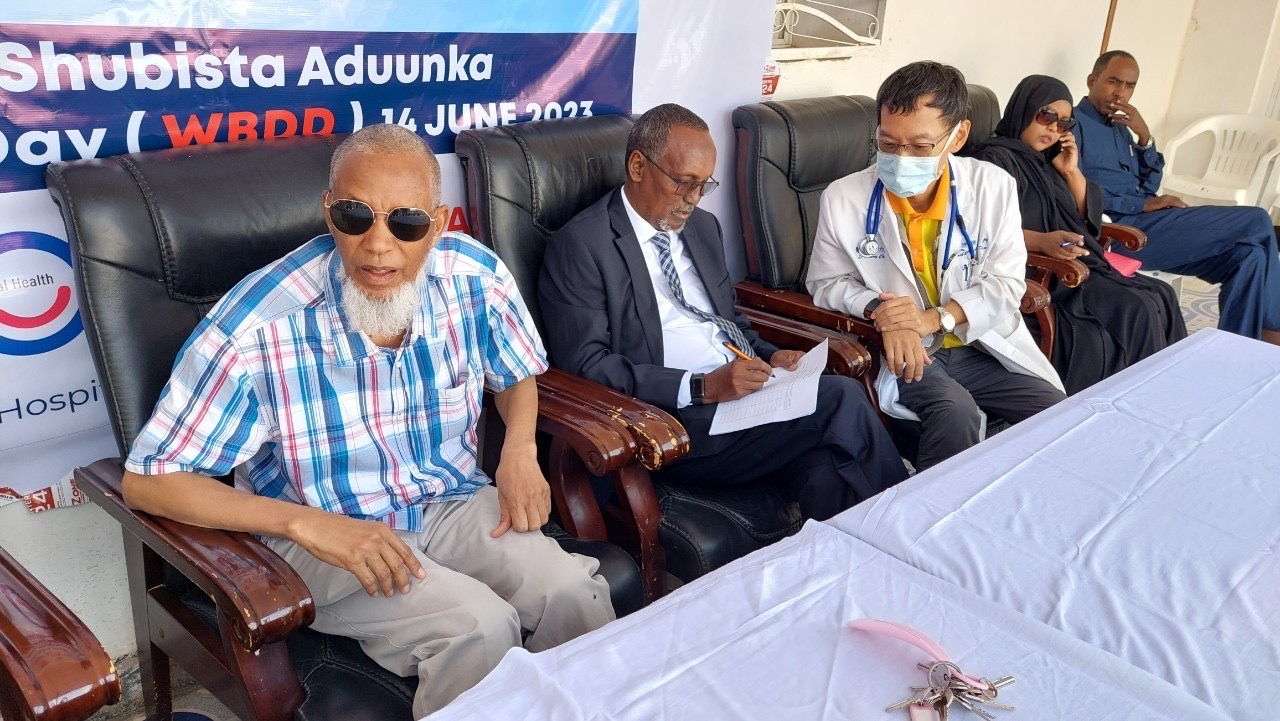
\includegraphics[width=0.75\textwidth]{IMG-4378.JPG}
    \end{center}
\end{frame}

% UoH student
\begin{frame}{Public health: World Blood Donor Day}
    \begin{center}
        \includesvg[width=0.2\textwidth]{Blood_logo.svg}
        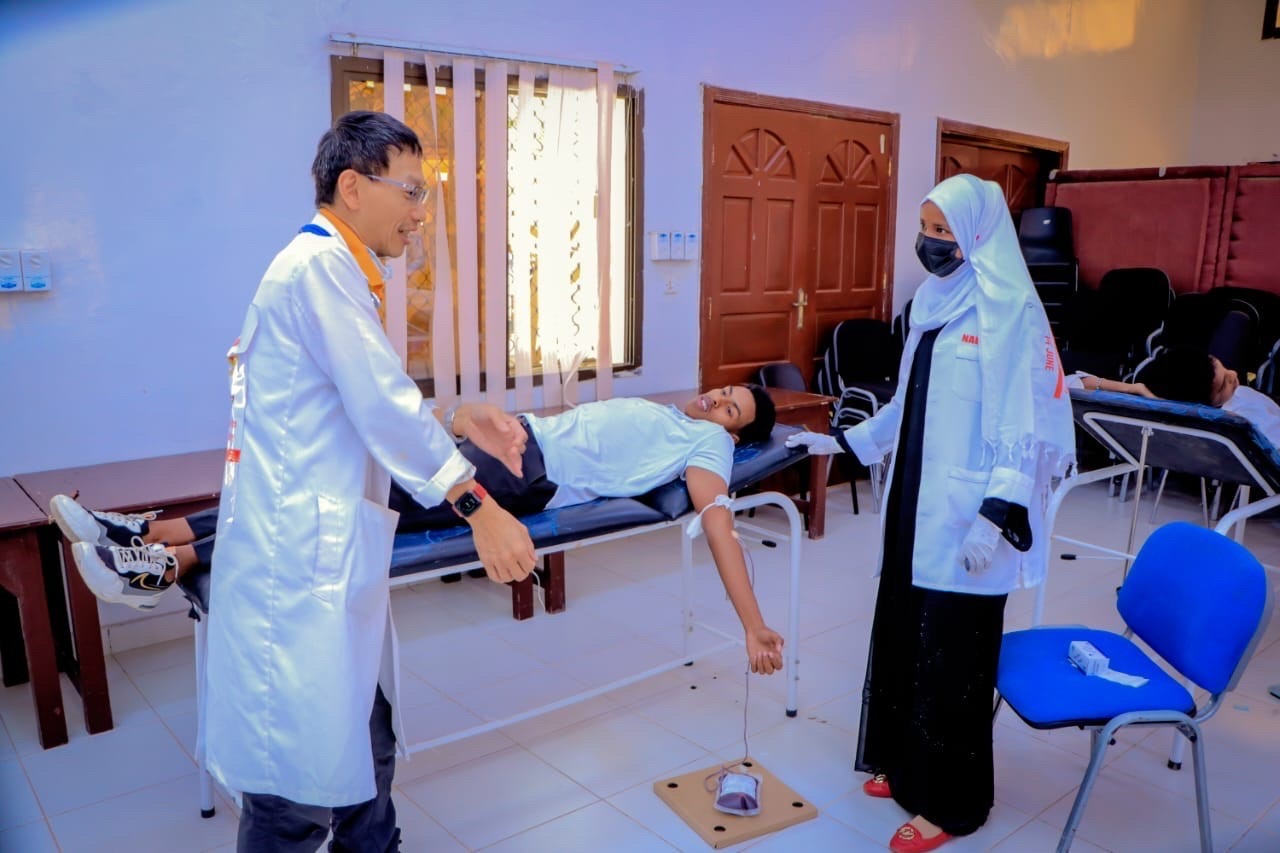
\includegraphics[width=0.45\textwidth]{IMG-5110.JPG}
        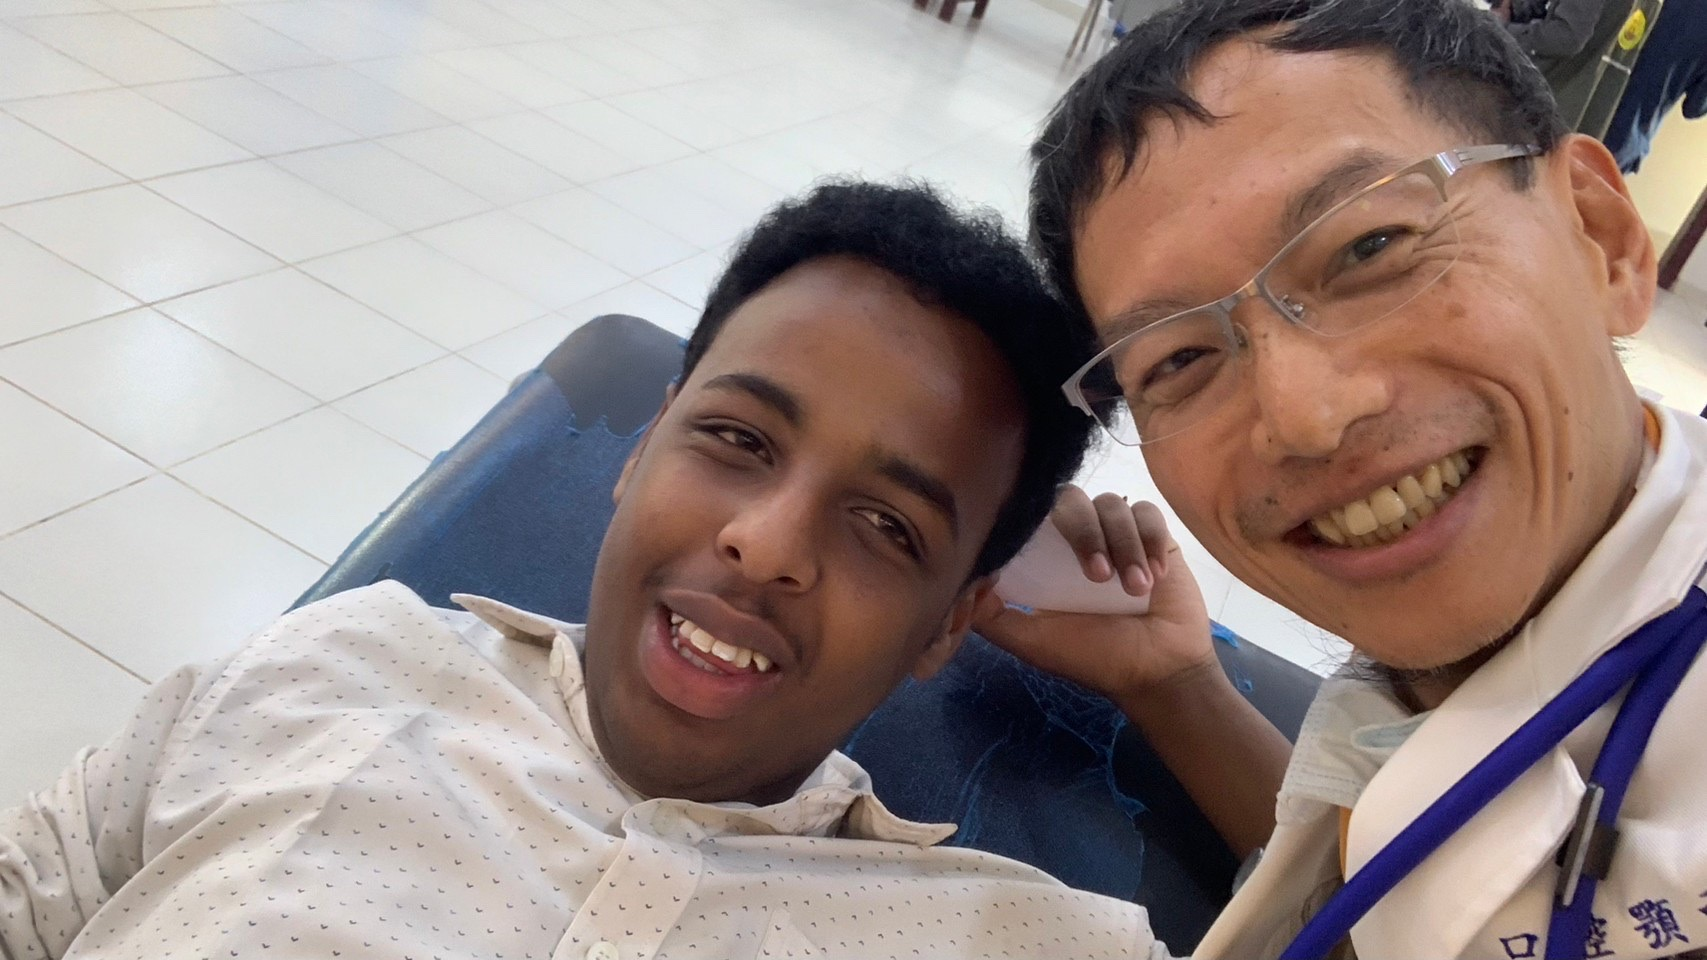
\includegraphics[width=0.25\textwidth]{IMG-5112.JPG}
    \end{center}
\end{frame}

\begin{frame}{Public health: World Blood Donor Day}
    \begin{center}
        \includesvg[width=0.2\textwidth]{Blood_logo.svg}
        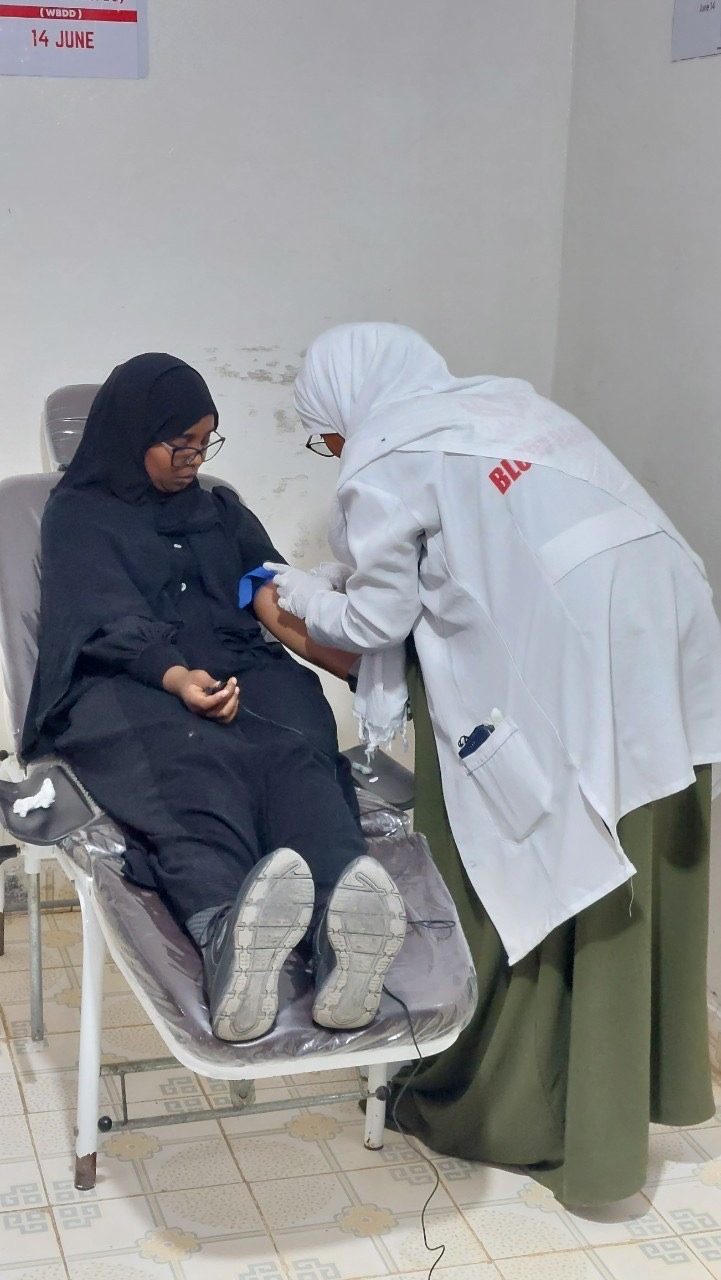
\includegraphics[width=0.30\textwidth]{IMG-4371.JPG}
        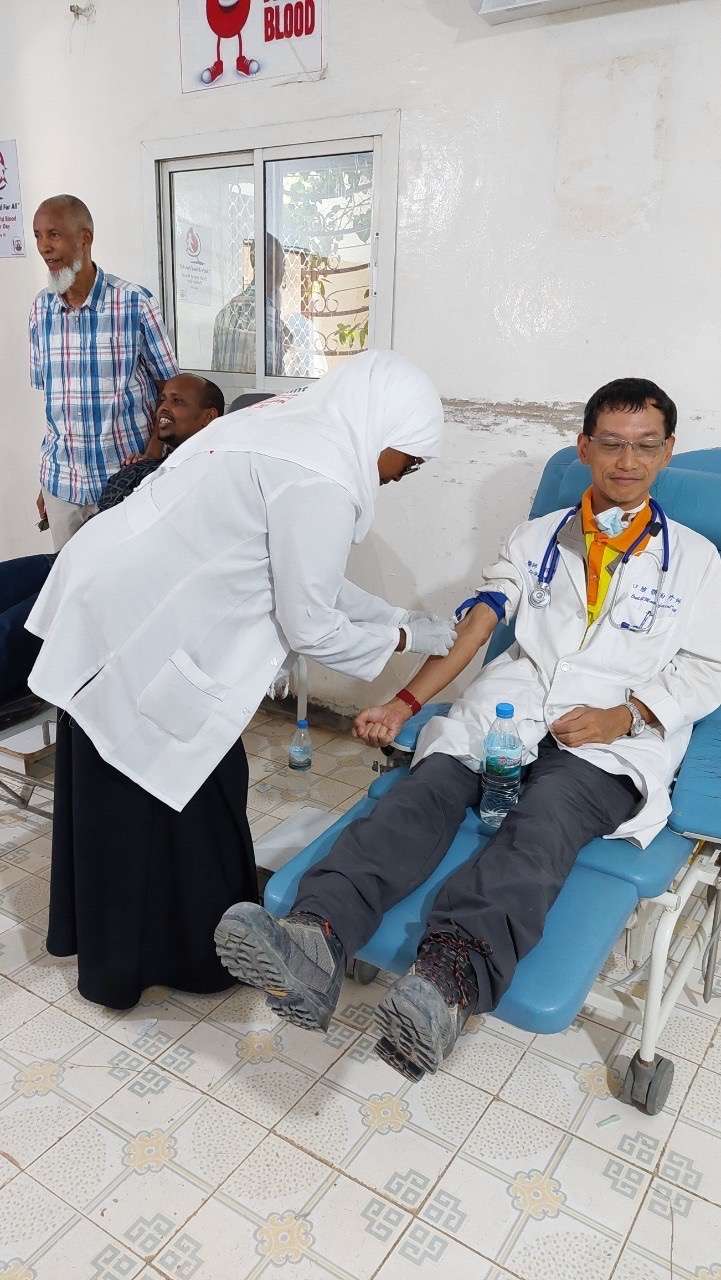
\includegraphics[width=0.30\textwidth]{IMG-4370.JPG}
    \end{center}
\end{frame}

\begin{frame}{Public health: World Blood Donor Day}
    \begin{center}
        \includesvg[width=0.2\textwidth]{Blood_logo.svg}
        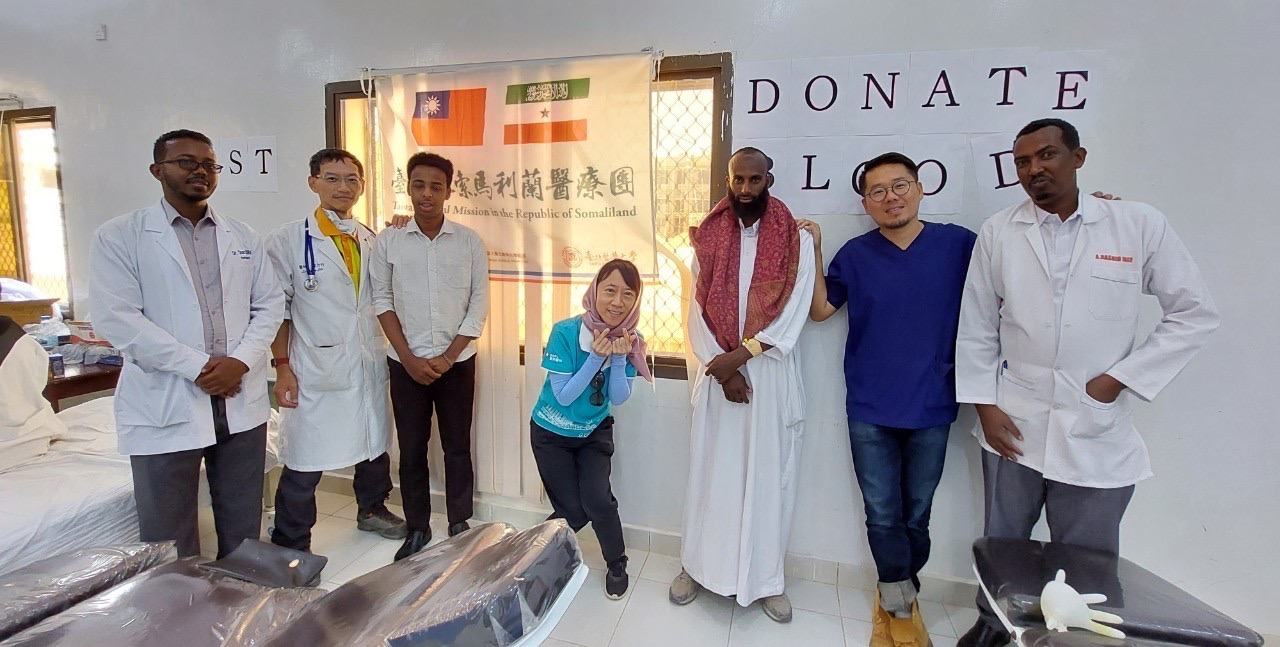
\includegraphics[width=0.75\textwidth]{IMG-4441.JPG}
%        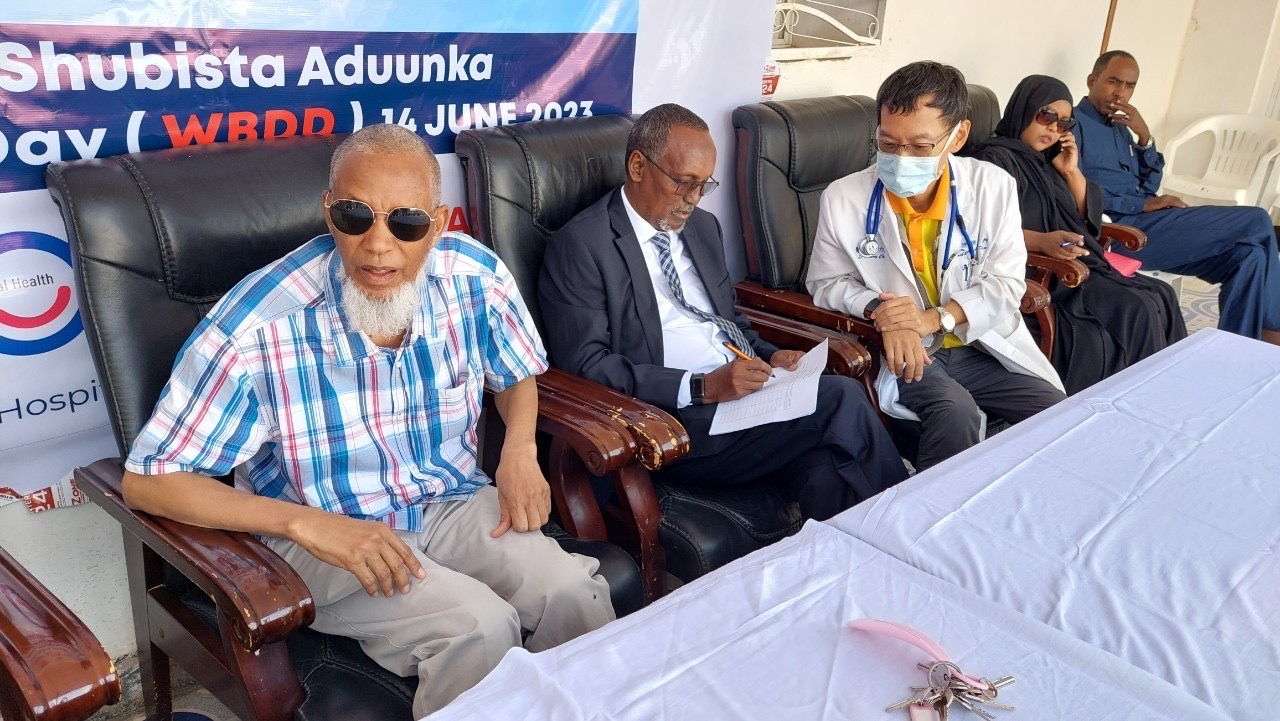
\includegraphics[width=0.45\textwidth]{IMG-4378.JPG}
    \end{center}
\end{frame}



%%%

\begin{frame}
\frametitle{TMM's Projects - fourth pillar}
% Add content here
\begin{outline}    
    \1 telemedicine
        \2 by collaborating with specialists at TMU affiliated Hospitals
        \2 telepathology project with a pathologist through digital whole-slide images (WSIs)
        \2 "RadiPush" project to fasciliate last-mile transfer of radiologist reports to doctors
    
\end{outline}
\end{frame}


\begin{frame}{Telepathology and Radiology}
    \begin{center}
        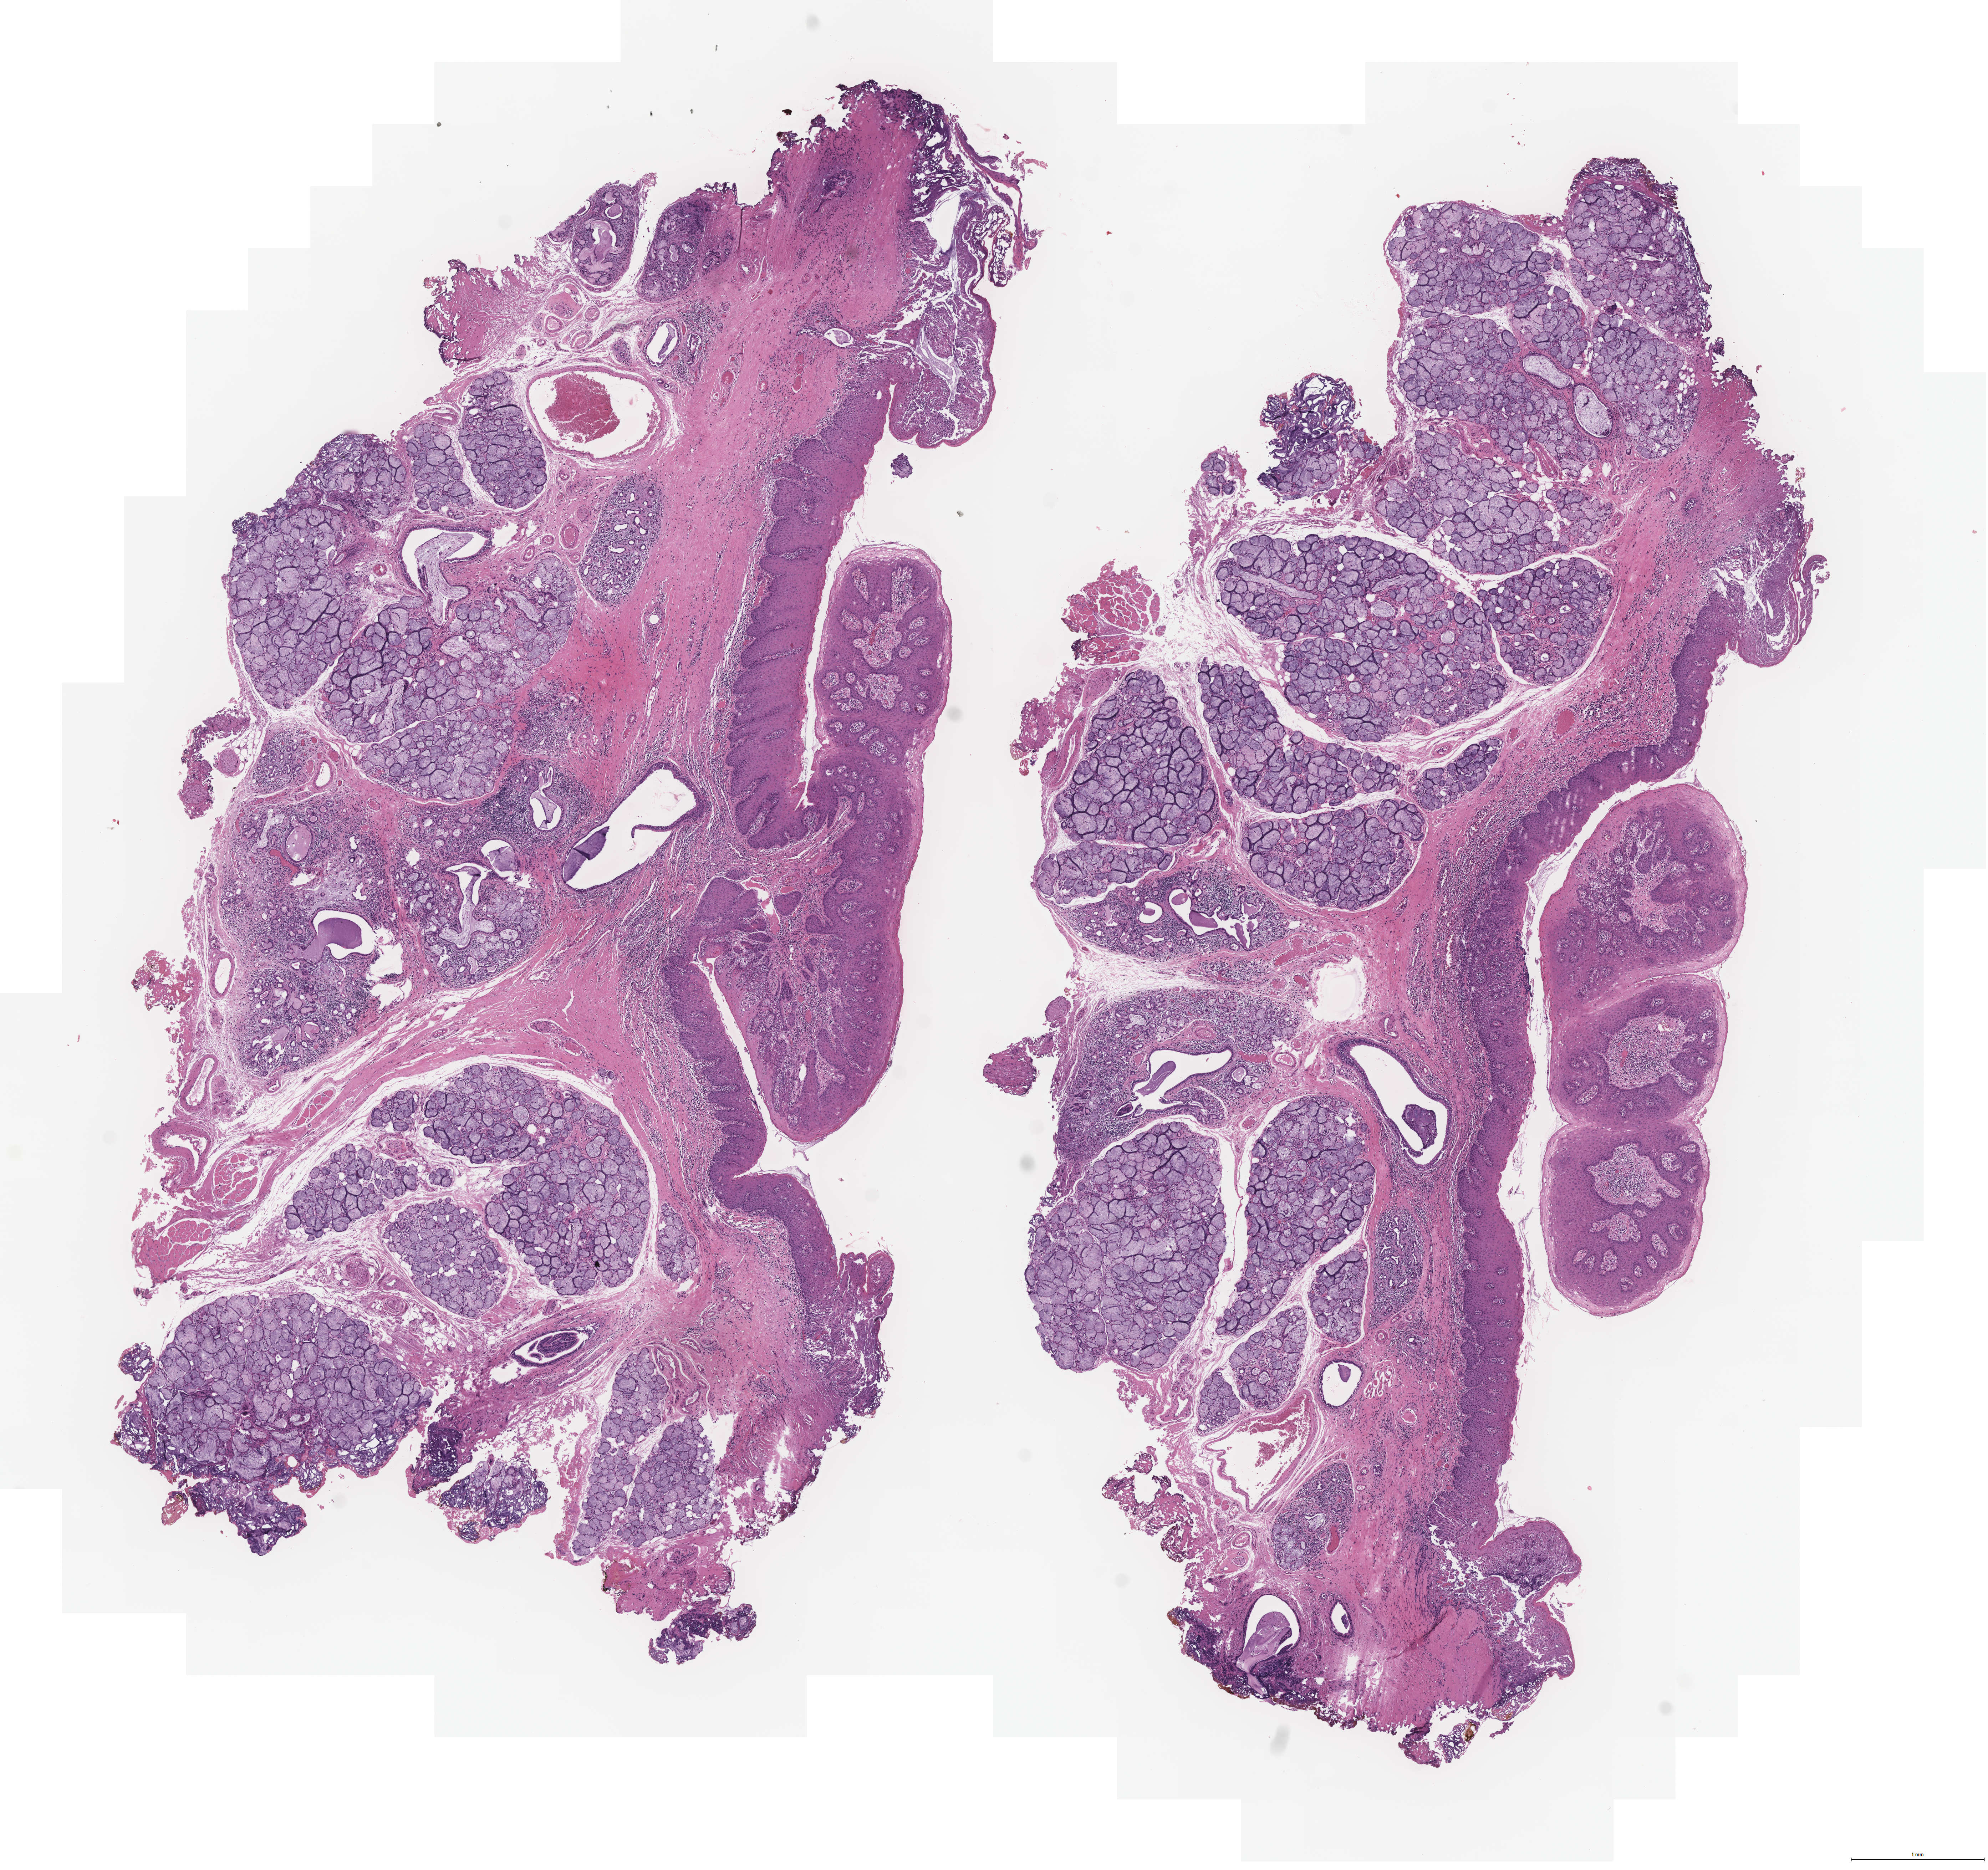
\includegraphics[width=0.35\textwidth]{TH1919729C1_HE.jpeg}
        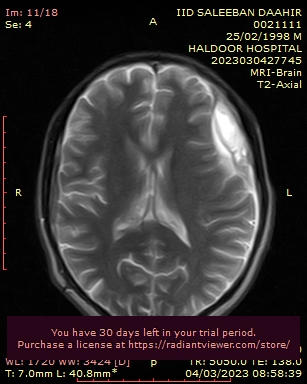
\includegraphics[width=0.30\textwidth]{IMG-0007-00001.jpg}
    \end{center}
\end{frame}


\begin{frame}{Teleconsultation: non-human vertebrae (cheetach)}
    \begin{center}
        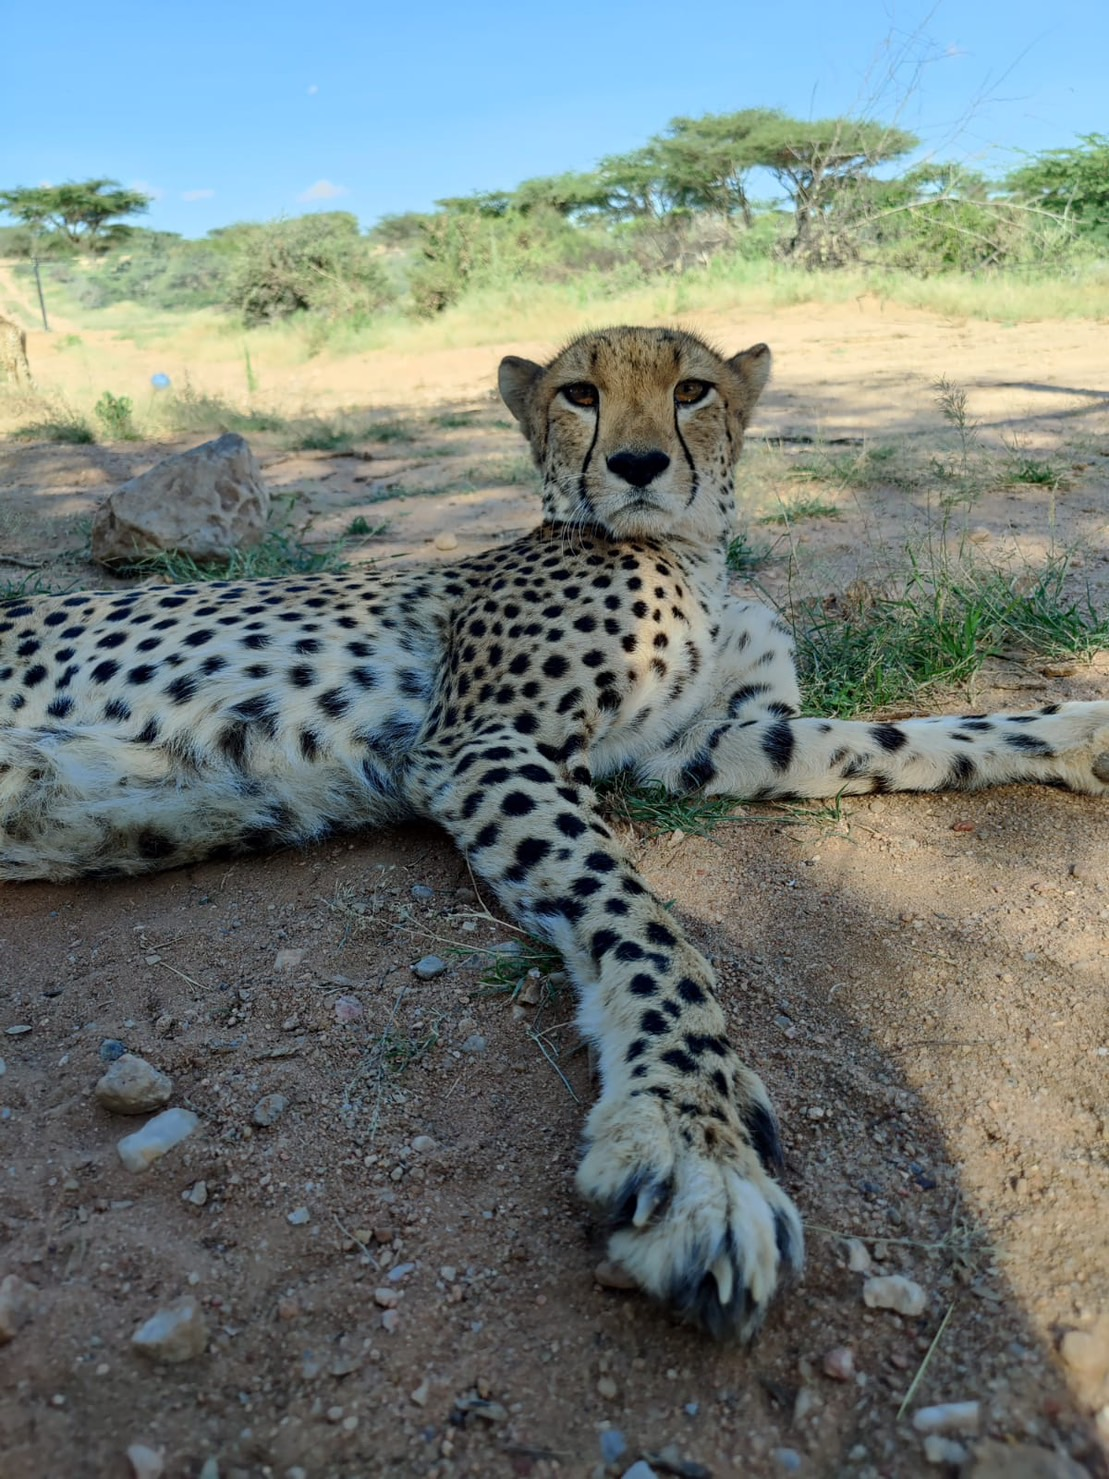
\includegraphics[width=0.35\textwidth]{457256160987709682.jpg}        \includegraphics[width=0.35\textwidth, origin=c,angle=180]{IMG-5116.JPG}

    \end{center}
\end{frame}
%%%%%%%%%%%%%
\section{Somaliland's Stories}

%% ultrasound baby
\begin{frame}
\frametitle{Happy mother "see" her baby}
% Add content here
\begin{center}
    \includegraphics[width=0.3\textwidth, trim=00mm 100mm 00mm 60mm,clip]{IMG-5117.JPG} 
    \includegraphics[width=0.3\textwidth, trim=60mm 60mm 30mm 60mm,clip]{52165_antenatal_check.jpg}

\end{center}
\end{frame}

%% Ismail oral cancer
\begin{frame}
\frametitle{"Welcome" grandfather going to sleep}
% Add content here
\begin{center}
\raisebox{70mm}{
    \includegraphics[width=0.8\textwidth, scale=-1,angle=180]{IMG-4861.jpg} 
    }
%    \includegraphics[width=0.3\textwidth, trim=60mm 60mm 30mm 60mm,clip]{52165_antenatal_check.jpg}

\end{center}
\end{frame}

%%%%%%%%%%
\section{Conclusion}
\begin{frame}
\frametitle{Thanks all of you}
% Add content here
\begin{center}
\raisebox{90mm}{
    \includegraphics[width=0.65\textwidth]{IMG-5017.JPG} 
    }
%    \includegraphics[width=0.3\textwidth, trim=60mm 60mm 30mm 60mm,clip]{52165_antenatal_check.jpg}

\end{center}
\end{frame}


%%
\begin{frame}
\frametitle{Take Home Message}
% Add content here
\begin{columns}
    
\column{0.4\textwidth}
\begin{outline}
    Our core value is:

\1 TMM offers medical professionals for people in need.
\1 TMM's presence is supposed to bring happiness and safety to everyone around them
%iby improving their health and well-being.
\1 TMM members have confidence, resilience, determination, and empathy when they face challenges.
\end{outline}

\column{0.6\textwidth}
\includegraphics[width=0.6\textwidth]{IMG-0394.JPG}
\end{columns}
\end{frame}

\begin{frame}{Trust me, Trust you}

\begin{columns}
    
\column{0.4\textwidth}
\begin{outline}
%Whenever TMM's members have short-term or long-term work in Somaliland,


\1 TMM members work as a team in Somaliland, whether they are there for a short time or for a long time.
\1 You can, however, think about how you can use the skills and experiences \textcolor{red}{you gained} here in your future job and life in Taiwan.
%\1 You can make the most of this time as a chance to learn and grow so that you can help us all get
%through \textcolor{blue}{the challenges} that we face here. 
%\1 We think that constant help is important for our overseas mission to be successful.

\end{outline}

\column{0.6\textwidth}
\includegraphics[width=0.7\textwidth]{IMG-5113.JPG}
\end{columns}

\end{frame}


%%%
\begin{frame}{Finale}
\begin{columns}
    
\column{0.4\textwidth}
\qrcode[height=2in]{https://www.facebook.com/profile.php?id=100094220689116&mibextid=LQQJ4d}
TMM facebook

\column{0.6\textwidth}
TMU白袍下的熱血---續集2023
\begin{outline}


    \1 人性面的溫暖,包容現實層面的無能為力
        \2 看病實況:一切自費,好似 1973 年代的臺灣
        \2 "他們"比起"我們"更能坦然接受死亡
        \2 \textcolor{red}{因為沒有很多,所以能捨}
    \1 當個非洲醫師的經驗,真好
%娓娓道來 

\end{outline}


\end{columns}
\end{frame}


%\end{CJK*}

\end{document}
